% Options for packages loaded elsewhere
\PassOptionsToPackage{unicode}{hyperref}
\PassOptionsToPackage{hyphens}{url}
%
\documentclass[
]{book}
\usepackage{amsmath,amssymb}
\usepackage{iftex}
\ifPDFTeX
  \usepackage[T1]{fontenc}
  \usepackage[utf8]{inputenc}
  \usepackage{textcomp} % provide euro and other symbols
\else % if luatex or xetex
  \usepackage{unicode-math} % this also loads fontspec
  \defaultfontfeatures{Scale=MatchLowercase}
  \defaultfontfeatures[\rmfamily]{Ligatures=TeX,Scale=1}
\fi
\usepackage{lmodern}
\ifPDFTeX\else
  % xetex/luatex font selection
\fi
% Use upquote if available, for straight quotes in verbatim environments
\IfFileExists{upquote.sty}{\usepackage{upquote}}{}
\IfFileExists{microtype.sty}{% use microtype if available
  \usepackage[]{microtype}
  \UseMicrotypeSet[protrusion]{basicmath} % disable protrusion for tt fonts
}{}
\makeatletter
\@ifundefined{KOMAClassName}{% if non-KOMA class
  \IfFileExists{parskip.sty}{%
    \usepackage{parskip}
  }{% else
    \setlength{\parindent}{0pt}
    \setlength{\parskip}{6pt plus 2pt minus 1pt}}
}{% if KOMA class
  \KOMAoptions{parskip=half}}
\makeatother
\usepackage{xcolor}
\usepackage{color}
\usepackage{fancyvrb}
\newcommand{\VerbBar}{|}
\newcommand{\VERB}{\Verb[commandchars=\\\{\}]}
\DefineVerbatimEnvironment{Highlighting}{Verbatim}{commandchars=\\\{\}}
% Add ',fontsize=\small' for more characters per line
\usepackage{framed}
\definecolor{shadecolor}{RGB}{248,248,248}
\newenvironment{Shaded}{\begin{snugshade}}{\end{snugshade}}
\newcommand{\AlertTok}[1]{\textcolor[rgb]{0.94,0.16,0.16}{#1}}
\newcommand{\AnnotationTok}[1]{\textcolor[rgb]{0.56,0.35,0.01}{\textbf{\textit{#1}}}}
\newcommand{\AttributeTok}[1]{\textcolor[rgb]{0.13,0.29,0.53}{#1}}
\newcommand{\BaseNTok}[1]{\textcolor[rgb]{0.00,0.00,0.81}{#1}}
\newcommand{\BuiltInTok}[1]{#1}
\newcommand{\CharTok}[1]{\textcolor[rgb]{0.31,0.60,0.02}{#1}}
\newcommand{\CommentTok}[1]{\textcolor[rgb]{0.56,0.35,0.01}{\textit{#1}}}
\newcommand{\CommentVarTok}[1]{\textcolor[rgb]{0.56,0.35,0.01}{\textbf{\textit{#1}}}}
\newcommand{\ConstantTok}[1]{\textcolor[rgb]{0.56,0.35,0.01}{#1}}
\newcommand{\ControlFlowTok}[1]{\textcolor[rgb]{0.13,0.29,0.53}{\textbf{#1}}}
\newcommand{\DataTypeTok}[1]{\textcolor[rgb]{0.13,0.29,0.53}{#1}}
\newcommand{\DecValTok}[1]{\textcolor[rgb]{0.00,0.00,0.81}{#1}}
\newcommand{\DocumentationTok}[1]{\textcolor[rgb]{0.56,0.35,0.01}{\textbf{\textit{#1}}}}
\newcommand{\ErrorTok}[1]{\textcolor[rgb]{0.64,0.00,0.00}{\textbf{#1}}}
\newcommand{\ExtensionTok}[1]{#1}
\newcommand{\FloatTok}[1]{\textcolor[rgb]{0.00,0.00,0.81}{#1}}
\newcommand{\FunctionTok}[1]{\textcolor[rgb]{0.13,0.29,0.53}{\textbf{#1}}}
\newcommand{\ImportTok}[1]{#1}
\newcommand{\InformationTok}[1]{\textcolor[rgb]{0.56,0.35,0.01}{\textbf{\textit{#1}}}}
\newcommand{\KeywordTok}[1]{\textcolor[rgb]{0.13,0.29,0.53}{\textbf{#1}}}
\newcommand{\NormalTok}[1]{#1}
\newcommand{\OperatorTok}[1]{\textcolor[rgb]{0.81,0.36,0.00}{\textbf{#1}}}
\newcommand{\OtherTok}[1]{\textcolor[rgb]{0.56,0.35,0.01}{#1}}
\newcommand{\PreprocessorTok}[1]{\textcolor[rgb]{0.56,0.35,0.01}{\textit{#1}}}
\newcommand{\RegionMarkerTok}[1]{#1}
\newcommand{\SpecialCharTok}[1]{\textcolor[rgb]{0.81,0.36,0.00}{\textbf{#1}}}
\newcommand{\SpecialStringTok}[1]{\textcolor[rgb]{0.31,0.60,0.02}{#1}}
\newcommand{\StringTok}[1]{\textcolor[rgb]{0.31,0.60,0.02}{#1}}
\newcommand{\VariableTok}[1]{\textcolor[rgb]{0.00,0.00,0.00}{#1}}
\newcommand{\VerbatimStringTok}[1]{\textcolor[rgb]{0.31,0.60,0.02}{#1}}
\newcommand{\WarningTok}[1]{\textcolor[rgb]{0.56,0.35,0.01}{\textbf{\textit{#1}}}}
\usepackage{longtable,booktabs,array}
\usepackage{calc} % for calculating minipage widths
% Correct order of tables after \paragraph or \subparagraph
\usepackage{etoolbox}
\makeatletter
\patchcmd\longtable{\par}{\if@noskipsec\mbox{}\fi\par}{}{}
\makeatother
% Allow footnotes in longtable head/foot
\IfFileExists{footnotehyper.sty}{\usepackage{footnotehyper}}{\usepackage{footnote}}
\makesavenoteenv{longtable}
\usepackage{graphicx}
\makeatletter
\def\maxwidth{\ifdim\Gin@nat@width>\linewidth\linewidth\else\Gin@nat@width\fi}
\def\maxheight{\ifdim\Gin@nat@height>\textheight\textheight\else\Gin@nat@height\fi}
\makeatother
% Scale images if necessary, so that they will not overflow the page
% margins by default, and it is still possible to overwrite the defaults
% using explicit options in \includegraphics[width, height, ...]{}
\setkeys{Gin}{width=\maxwidth,height=\maxheight,keepaspectratio}
% Set default figure placement to htbp
\makeatletter
\def\fps@figure{htbp}
\makeatother
\setlength{\emergencystretch}{3em} % prevent overfull lines
\providecommand{\tightlist}{%
  \setlength{\itemsep}{0pt}\setlength{\parskip}{0pt}}
\setcounter{secnumdepth}{5}
\usepackage{booktabs}
\ifLuaTeX
  \usepackage{selnolig}  % disable illegal ligatures
\fi
\usepackage[]{natbib}
\bibliographystyle{plainnat}
\usepackage{bookmark}
\IfFileExists{xurl.sty}{\usepackage{xurl}}{} % add URL line breaks if available
\urlstyle{same}
\hypersetup{
  pdftitle={MANUAL DE R Y RSTUDIO},
  pdfauthor={Stephanie Hereira-Pacheco; Mauricio Hernández},
  hidelinks,
  pdfcreator={LaTeX via pandoc}}

\title{MANUAL DE R Y RSTUDIO}
\author{Stephanie Hereira-Pacheco \and Mauricio Hernández}
\date{}

\begin{document}
\maketitle

{
\setcounter{tocdepth}{1}
\tableofcontents
}
\chapter*{Prefacio}\label{prefacio}
\addcontentsline{toc}{chapter}{Prefacio}

Este libro contiene la recopilación de temas impartidos y tratados a lo largo de diferentes cursos y lecciones sobre R y sus aplicaciones en Ciencias Biológicas.

\section{Objetivo del libro}\label{objetivo-del-libro}

Que los estudiantes de nivel pregrado y posgrado puedan aprender temas básicos y aplicados del lenguaje de R y su aplicación en sus estudios y trabajos enfocados en ciencias biológicas.

\section{\texorpdfstring{\textbf{Requisitos}}{Requisitos}}\label{requisitos}

\begin{itemize}
\tightlist
\item
  Rstudio versiones 2024 en adelante.
\item
  R versiones de 4.0 en adelante.
\end{itemize}

\section{Instalación de Rsudio y R}\label{instalaciuxf3n-de-rsudio-y-r}

En caso de no tener instalado Rstudio y R que son los prerequisitos para llevar a cabo los ejercicios y temas de est elibro, entonces visita estas ligas para descargarlos e instalarlos.

\subsection{Rstudio}\label{rstudio}

\begin{itemize}
\tightlist
\item
  En \href{https://download1.rstudio.org/electron/macos/RStudio-2024.12.1-563.dmg}{MacOS}
\item
  En \href{https://download1.rstudio.org/electron/jammy/amd64/rstudio-2024.12.1-563-amd64.deb}{Ubuntu}
\item
  En \href{https://download1.rstudio.org/electron/windows/RStudio-2024.12.1-563.exe}{Windows}
\end{itemize}

\subsection{R}\label{r}

\begin{itemize}
\tightlist
\item
  Para \href{https://cran.r-project.org/bin/macosx/}{MacOS}
\item
  Para \href{https://cran.r-project.org/bin/linux/ubuntu/}{Ubuntu}
\item
  Para \href{https://cran.r-project.org/bin/windows/base/}{Windows}
\end{itemize}

\section{Aviso Legal: Protección de Propiedad Intelectual.}\label{aviso-legal-protecciuxf3n-de-propiedad-intelectual.}

El material contenido en este manual está protegido por las leyes mexicanas de Propiedad Intelectual. Por lo que su reproducción o distribución no autorizada con fines de lucro está prohibida.

\chapter{: Introducción a R}\label{introducciuxf3n-a-r}

\section{Comenzando con R y RStudio}\label{getting-started}

\subsection{Breve descripción de R}\label{breve-descripciuxf3n-de-r}

R es un lenguaje de programación como C o Java o Python pero enfocado principalmente a la estadística.
No fue creado por ingenieros de software para el desarrollo de software, sino por estadísticos como un ambiente interactivo para el análisis de datos.
Otros programas como los que mencioné anteriormente sí están más enfocados en el desarrollo de programas aunque también pueden usarse para hacer cálculos estadísticos.
Cuando instalamos R en nuestra computadora en realidad lo que estamos instalando es el entorno computacional y para que podamos hacer uso de ese entorno necesitamos conocer la manera de escribir que el software pueda interpretar y ejecutar las instrucciones que le damos.
Eso es lo que aprenderemos a hacer en este curso.

Como en otros lenguajes de programación, en R pueden guardar su trabajo como una secuencia de comandos o instrucciones, conocida como un \emph{script}, que se pueden ejecutar fácilmente en cualquier momento, los podemos guardar y nos servirań siempre.

\subsection[Un poco de historia\ldots{}]{\texorpdfstring{Un poco de historia\ldots{}\footnote{\url{https://bookdown.org/ndphillips/YaRrr/arranging-plots-with-parmfrow-and-layout.html}}}{Un poco de historia\ldots{}}}\label{un-poco-de-historia1}

R proviene del lenguaje S, creado en los Laboratorios Bell (Estados Unidos).
Los mismos que inventaron el transistor, el láser, el sistema operativo Unix y algunas otras cosas más.

Ross Ihaka y Robert Gentleman, de la Universidad de Auckland de Nueva Zelanda, decidieron crear una implementación abierta y gratuita de S.
Este trabajo, que culminaría en la creación de R inició en 1992 y no fue hasta el 2000 que se obtuvo una versión final estable.

Hoy día, el mantenimiento y desarrollo de R es realizado por el R Development Core Team, un equipo de especialistas en ciencias computacionales y estadística provenientes de diferentes instituciones y lugares alrededor del mundo.

R posee una Licencia Pública General de GNU, esto, para que pueda ser distribuido de manera gratuita, por lo que es software libre y de código abierto.
Esta licencia también te permite usar R para los fines que desees, sin limitaciones, no importando si son personales, académicos o comerciales.

\subsection[¿Por qué usar R?]{\texorpdfstring{¿Por qué usar R?\footnote{\url{https://cran.r-project.org/web/packages/cowplot/vignettes/introduction.html}}}{¿Por qué usar R?}}\label{por-quuxe9-usar-r2}

\begin{enumerate}
\def\labelenumi{\arabic{enumi}.}
\tightlist
\item
  R es gratuito y de código abierto\footnote{\url{https://cran.r-project.org/web/packages/egg/vignettes/Ecosystem.html}}.
\item
  Se ejecuta en todas las plataformas principales: Windows, Mac Os, UNIX/Linux.
\item
  Los \emph{scripts} y los objetos de datos se pueden compartir sin problemas entre plataformas.
\item
  Existe una comunidad grande, creciente y activa de usuarios de R y, como resultado, hay numerosos recursos para aprender y hacer preguntas\footnote{\url{https://r-charts.com/es/miscelanea/}} \footnote{\url{https://www.r-project.org/help.html}}.
\item
  Es fácil para otras personas contribuir con complementos (\emph{add-ons} en inglés) o paquetes que les permiten a los desarrolladores compartir implementaciones de software de nuevas metodologías de ciencia de datos. Esto les da a los usuarios de R acceso temprano a los métodos y herramientas más recientes que se desarrollan para una amplia variedad de disciplinas, incluyendo la ecología, la biología molecular, las ciencias sociales y la geografía, entre otros campos.
\end{enumerate}

\subsection{RStudio}\label{rstudio}

RStudio será nuestra plataforma para los proyectos usados con el lenguaje R.
Nos provee un editor visual e interactivo para crear y editar nuestros \emph{scripts}, además de otras herramientas útiles que iremos viendo con el pasar de los temas.

\subsection{Interfaz de Rstudio}\label{interfaz-de-rstudio}

Rstudio posee 4 paneles principales:

\begin{enumerate}
\def\labelenumi{\arabic{enumi}.}
\item
  El panel izquierdo superior aparece nuestro editor de códigos.
  Donde ponemos los scripts que vamos a correr.
\item
  A la derecha, el panel superior incluye pestañas como \emph{Environment} y \emph{History}, que son el ambiente y el historial, aquí podremos observar los objetos que vayamos declarando y data que subamos, además del historial de scripts.
\item
  En el panel inferior izquierdo nos aparece nuestra consola de R que es donde se corren los códigos.
\item
  En el panel inferior derecho se muestran cinco pestañas: \emph{File}, \emph{Plots}, \emph{Packages}, \emph{Help} y \emph{Viewer}.
  Pueden hacer clic en cada pestaña para moverse por las diferentes opciones.
  Pero a grandes rasgos, en file vemos donde nos encontramos situados y los archivos que hay en nuestro directorio.
  En plots se visualizan las imágenes que generamos, en packages los paquetes que poseemos instalados y cargados, en Help cuando necesitamos información extra de nuestros paquetes y en Viewer exploramos scripts de rmarkdown.
\end{enumerate}

\hfill\break

\begin{center}\includegraphics[width=300pt]{images/Consola2} \end{center}

\subsection{\texorpdfstring{\emph{Scripts}}{Scripts}}\label{scripts}

Una de las grandes ventajas de R y Rstudio es que se pueden guardar los diversos códigos e instrucciones, los famosos conocidos como \emph{scripts}, que entonces se pueden editar y guardar con un editor de texto.

Para iniciar un nuevo \emph{script}, hagan clic en \emph{Archivo}, entonces \emph{Nuevo Archivo} y luego \emph{R Script}.
Esto inicia un nuevo panel a la izquierda y es aquí donde pueden comenzar a escribir su \emph{script}.\\

\includegraphics[width=0.5\linewidth]{images/script}
\includegraphics[width=0.5\linewidth]{images/script2}

\hfill\break

Podemos abrir y ejecutar scripts en R usando la función source(), dandole como argumento la ruta del archivo .R en nuestra computadora, entre comillas o yendo a \emph{File}, entonces \emph{Open File} y luego buscando en las carpetas donde tengas el script.

Por ejemplo.

\begin{Shaded}
\begin{Highlighting}[]
\FunctionTok{source}\NormalTok{(}\StringTok{"C:/mi\_script.R"}\NormalTok{)}
\end{Highlighting}
\end{Shaded}

\subsubsection{\texorpdfstring{Cómo ejecutar comandos mientras editan \emph{scripts}}{Cómo ejecutar comandos mientras editan scripts}}\label{cuxf3mo-ejecutar-comandos-mientras-editan-scripts}

Empezamos por abrir un nuevo \emph{script} y luego nombramos el \emph{script}.
Podemos hacer esto a través del editor guardando el nuevo \emph{script} actual sin nombre.
Al guardar el script por primera vez use un nombre descriptivo, con letras minúsculas, sin espacios, preferiblemente con ``\_'' para separar palabras, evitar guiones ``-'' para separar las palabras.
Llamaremos a este \emph{script}: \emph{mi\_script.R}.\\

\begin{center}\includegraphics[width=300pt]{images/save} \end{center}

Ahora podemos editar nuestro primer \emph{script}.

Las primeras líneas de código son títulos o comentarios, para hacerlo siempre debemos poner el símbolo \emph{``\#''} para indicar que no es un código y luego cargamos los paquetes y datos que vamos a utilizar.
Para esta parte, luego veremos otra sección donde profundizaremos mejor en esto de cargar datos y paquetes.

Ahora podemos continuar escribiendo código.
Como ejemplo, trabajaremos con \emph{``iris''} dataset.
Cargamos la librería \emph{``datasets''} y cargamos la data, luego veremos el resumen de los datos y por último graficaremos un boxplot.
Para hacer esto, escribimos cada línea de código y luego hacemos click en el botón \emph{Run} en la parte derecha superior del panel de edición.
Para ejecutar una línea pueden usar Control+Enter en Windows y Linux y Command+Return en Mac.

Estas son las líneas del código:

\begin{Shaded}
\begin{Highlighting}[]
\FunctionTok{library}\NormalTok{(datasets)}
\FunctionTok{data}\NormalTok{(iris)}
\FunctionTok{summary}\NormalTok{(iris)}
\FunctionTok{boxplot}\NormalTok{(iris)}
\end{Highlighting}
\end{Shaded}

Y así luce al correrlo:\\

\includegraphics[width=500pt]{images/code}

\hfill\break

Tan pronto se corra el código, aparece en la consola y el gráfico aparece en en panel de \emph{``Plots''} , este panel permite hacer click hacia delante o hacia atrás en diferentes gráficos, hacer zoom en el gráfico o guardar los gráficos como archivos.

\subsection{Directorio de trabajo}\label{directorio-de-trabajo}

El \emph{directorio de trabajo} es el lugar en nuestra computadora en el que se encuentran los archivos con los que estamos trabajando en R.
Este es el lugar donde R busca los archivos para importarlos y al que serán exportados o guardados, a menos que se indique otra cosa.

Para saber donde está ubicado tu directorio de trabajo, puedes poner el código:

\begin{Shaded}
\begin{Highlighting}[]
\FunctionTok{getwd}\NormalTok{()}
\end{Highlighting}
\end{Shaded}

Y para establecer o cambiar este directorio de trabajo, correr el siguiente código:

\begin{Shaded}
\begin{Highlighting}[]
\FunctionTok{setwd}\NormalTok{(}\StringTok{"/home/steph/Desktop/"}\NormalTok{)}
\end{Highlighting}
\end{Shaded}

Por ejemplo en este caso estoy estableciendo mi directorio de trabajo en la carpeta ``Escritorio''.
También si se quiere conocer el contenido de tu directorio, como archivos o directorios puedes usar los siguientes códigos:

\begin{Shaded}
\begin{Highlighting}[]
\FunctionTok{list.files}\NormalTok{()}
\FunctionTok{list.dirs}\NormalTok{()}
\end{Highlighting}
\end{Shaded}

\subsection{Sesión}\label{sesiuxf3n}

Los objetos y funciones de R son almacenados en la memoria de nuestra computadora.
Cuando ejecutamos R, ya estamos creando una instancia del entorno computacional de este lenguaje de programación, cada instancia es una \emph{sesión}.

Todos los objetos, tablas, gráficas y funciones creadas en una sesión, permanecen sólo en ella, no son compartidos entre sesiones.
Si se quiere guardar toda esta data generada en la sesión antes de cerrar el R hay que indicar que se guarde, sino, aunque se guarden los scripts, los objetos (que algunos pueden ser muy pesados y ocupar memoria) no se guardarán.
Lo cual es una opción si no se tiene mucho espacio en el disco.
Es posible tener más de una sesión de R activa en la misma computadora.
Esto se guarda en un archivo con extensión **.Rdata* en tu directorio de trabajo.

Con la función \emph{ls()} conoceremos una lista con los nombres de todo lo guardado en la sesión.
En las siguientes imágenes ilustro como crear un nuevo proyecto:

\subsection{Proyecto}\label{proyecto}

Un proyecto de R (extensión .Rproj) identifica todos los archivos y contenido asociado con él.
Ayuda a organizar tu trabajo y así cada curso, artículo o trabajo diferente puede tener un proyecto diferente.
Al crear un proyecto todos los ficheros quedan vinculados directamente a él.\\

\begin{center}\includegraphics[width=400pt]{images/new_directory} \end{center}

\hfill\break

\begin{center}\includegraphics[width=400pt]{images/new_directory2} \end{center}

\hfill\break

\begin{center}\includegraphics[width=400pt]{images/new_directory3} \end{center}

\hfill\break

\subsection{Instalación de paquetes de R}\label{instalaciuxf3n-de-paquetes-de-r}

Dentro de las ventajas de R está que muchos desarrolladores y programadores elaboran constantemente complementos, aplicaciones o en palabras propias \emph{paquetes} que nos permiten usar en acceso libre y que tienen muchas funcionalidades.
Actualmente hay muchos disponibles en CRAN (Comprehensive R Archive Network) que es una red de servidores alrededor del mundo que almacena versiones actualizadas del código de R y su documentación.
También hay muchos paquetes desarrollados publicados en GitHub y en Bioconductor.
Por ejemplo para instalar el paquete tidyverse, que es de gran utilidad y que veremos en sesiones posteriores, usamos el código:

\begin{Shaded}
\begin{Highlighting}[]
\FunctionTok{install.packages}\NormalTok{(}\StringTok{"tidyverse"}\NormalTok{)}
\end{Highlighting}
\end{Shaded}

En RStudio pueden navegar a la pestaña \emph{Pakages} y seleccionar \emph{Install}.
Luego, escribir el paquete que queremos siempre y cuando esté en CRAN.
Para cargar una librería como lo vimos anteriormente se usa la función, \texttt{library()}:

\begin{Shaded}
\begin{Highlighting}[]
\FunctionTok{library}\NormalTok{(tidyverse)}
\end{Highlighting}
\end{Shaded}

Una vez que se instalan los paquetes, no deben instalarlo de nuevo, sin embargo, cada vez que cerramos sesión, reiniciamos sesión o abrimos un nuevo proyecto o sesión tenemos que volver a cargarlos.

Debemos tener en cuenta que la instalación de \textbf{tidyverse} instala varios paquetes.
Esto ocurre comúnmente cuando un paquete tiene \emph{dependencias}, es decir usa funciones de otros paquetes.
Cuando cargan un paquete usando \texttt{library}, también cargan sus dependencias.

Hay paquetes que no se encuentra en CRAN o que si queremos su versión en desarrollo, se necesitan de otros paquetes para ser instalados, por ejemplo, si queremos instalar la versión en desarrollo del paquete \emph{``rmarkdown''}, que se encuentra en github, se utiliza el paquete devtools:

\begin{Shaded}
\begin{Highlighting}[]
\NormalTok{devtools}\SpecialCharTok{::}\FunctionTok{install\_github}\NormalTok{(}\StringTok{\textquotesingle{}rstudio/rmarkdown\textquotesingle{}}\NormalTok{)}
\end{Highlighting}
\end{Shaded}

Los dos puntos \emph{``::''} se utilizan para denotar que llamamos la función de un paquete pero sin llamarla permanentemente en nuestra sesión.

\subsection{Tipos de objetos en R}\label{tipos-de-objetos-en-r}

La información que manipulamos en R se estructura en forma de objetos y los podemos ver almacenados en el panel del ambiente de trabajo o \emph{Enviroment}.
Los objetos pueden ser:

\begin{itemize}
\item
  Números escalares o letras
\item
  Vectores y matrices
\item
  Dataframes, tablas y listas
\end{itemize}

Más adelante detallaremos este tipo de objetos o datos en R.
Aquí unos ejemplos:

\begin{Shaded}
\begin{Highlighting}[]
\NormalTok{a }\OtherTok{\textless{}{-}} \DecValTok{1}                                                          \CommentTok{\#escalar}
\NormalTok{letra }\OtherTok{\textless{}{-}} \StringTok{"a"}                                                    \CommentTok{\#caracter o letra}
\NormalTok{b }\OtherTok{\textless{}{-}} \FunctionTok{c}\NormalTok{(}\DecValTok{1}\NormalTok{,}\DecValTok{2}\NormalTok{,}\DecValTok{3}\NormalTok{)                                                   }\CommentTok{\#vector}
\NormalTok{c}\OtherTok{\textless{}{-}} \FunctionTok{matrix}\NormalTok{(}\DecValTok{1}\SpecialCharTok{:}\DecValTok{10}\NormalTok{)                                                }\CommentTok{\#matriz}
\NormalTok{d}\OtherTok{\textless{}{-}} \FunctionTok{data.frame}\NormalTok{(}\AttributeTok{Especie=}\FunctionTok{c}\NormalTok{(}\StringTok{"A"}\NormalTok{, }\StringTok{"B"}\NormalTok{), }\AttributeTok{Longitud=}\FunctionTok{c}\NormalTok{(}\FunctionTok{c}\NormalTok{(}\DecValTok{1}\NormalTok{,}\DecValTok{2}\NormalTok{)))         }\CommentTok{\#dataframe o tabla}
\NormalTok{e}\OtherTok{\textless{}{-}} \FunctionTok{list}\NormalTok{(}\FunctionTok{c}\NormalTok{(}\DecValTok{1}\SpecialCharTok{:}\DecValTok{20}\NormalTok{), }\FunctionTok{c}\NormalTok{(}\DecValTok{1}\SpecialCharTok{:}\DecValTok{10}\NormalTok{))                                      }\CommentTok{\#lista}
\end{Highlighting}
\end{Shaded}

Una ventaja de los lenguajes de programación es poder definir variables y escribir expresiones como estas, como se hace en las matemáticas y así almacenar los valores para su uso posterior.
Usamos \texttt{\textless{}-} para asignar valores a las variables.
También podemos asignar valores usando \texttt{=} en lugar de \texttt{\textless{}-}, pero recomendamos no usar \texttt{=}.
Esto, debido a que en R el signo \texttt{=} implica igualdad en términos lógicos y no asignación y esto puede evitarnos confusiones en el futuro.

Para ver el valor almacenado en una variable, simplemente le pedimos a R que evalúe \texttt{a} y R nos muestra el valor almacenado:

\begin{Shaded}
\begin{Highlighting}[]
\NormalTok{a}
\end{Highlighting}
\end{Shaded}

\begin{verbatim}
## [1] 1
\end{verbatim}

Una forma explícita de pedirle a R que nos muestre el valor almacenado en \texttt{a} es usar \texttt{print} así:

\begin{Shaded}
\begin{Highlighting}[]
\FunctionTok{print}\NormalTok{(a)}
\end{Highlighting}
\end{Shaded}

\begin{verbatim}
## [1] 1
\end{verbatim}

Otra forma de examinar los objetos es buscarlos en el \emph{Enviorment} o ambiente de trabajo y visualizarlos desde allí.
Deberíamos ver \texttt{a}, \texttt{b} y las que ya hemos declarado en el ambiente.
Si intentamos imprimir o visualizar el valor de un objeto que no está definido en el ambiente se recibirá un mensaje de error.
Por ejemplo, si escriben \texttt{f}, verán lo siguiente: \texttt{Error:\ object\ \textquotesingle{}f\textquotesingle{}\ not\ found}.

\paragraph{Algunos tips para asignar variables u objetos en R\ldots{}}\label{algunos-tips-para-asignar-variables-u-objetos-en-r}

\begin{itemize}
\item
  Los nombres de variables tienen que comenzar con una letra, no pueden contener espacios y no deben ser variables predefinidas en R (como funciones o argumentos de funciones).
  Por ejemplo, no nombren una de sus variables \texttt{install.packages} escribiendo algo como: \texttt{install.packages\ \textless{}-\ 2}.
  Esto reescribe la función o causa confusiones para R.
\item
  Que tus nombres sean descriptivos y/o significativos para lo que se está almacenado, usar solo minúsculas y usar guiones bajos \emph{( \_ )} como sustituto de espacios, evitar caracteres especiales (- ; . @ ?) .
\end{itemize}

\subsubsection{Guardar los espacios de trabajo y exportar objetos de R}\label{guardar-los-espacios-de-trabajo-y-exportar-objetos-de-r}

Los objetos evaluados permanecen en el espacio de trabajo hasta que finalicen sus sesiones sin guardar.
Pero los espacios de trabajo también se pueden guardar para su uso posterior.
De hecho, al salir de R, el programa les pregunta si desean guardar su espacio de trabajo.
Si lo guardan, la próxima vez que inicien R, el programa restaurará el espacio de trabajo con todos los objetos en él.

Sin embargo, no se recomienda guardar el espacio de trabajo porque sino se trabaja con diferentes proyectos, será más difícil darle seguimiento de lo que guardan y ocupara mucho espacio en la memoria de su disco.
En cambio, se recomienda en gran medida realizar un proyecto por trabajo o tarea y así tener un espacio de trabajo para cada uno.
Decidiendo o no si guardar las sesiones y no entrar en confusiones entre las diferentes sesiones.

Ahora bien R ya posee funciones de exporte, tales como:

\begin{Shaded}
\begin{Highlighting}[]
\FunctionTok{library}\NormalTok{(readr)}
\FunctionTok{write\_tsv}\NormalTok{(d, }\StringTok{"data.tsv"}\NormalTok{)}
\FunctionTok{write.table}\NormalTok{(d, }\StringTok{"data.txt"}\NormalTok{, }\AttributeTok{sep =} \StringTok{"}\SpecialCharTok{\textbackslash{}t}\StringTok{"}\NormalTok{)}
\FunctionTok{write\_csv}\NormalTok{(d, }\StringTok{"data.csv"}\NormalTok{)}
\end{Highlighting}
\end{Shaded}

Estas funciones guardan tus tablas u objetos con formatos de texto.
También hay una forma de guardar objetos de R sin declararlos como texto sino que se queden con la identidad de R:

\begin{Shaded}
\begin{Highlighting}[]
\FunctionTok{saveRDS}\NormalTok{(d, }\StringTok{"data.RDS"}\NormalTok{)}
\end{Highlighting}
\end{Shaded}

Y para abrir o cargar este tipo de objetos con extensión .RDS usamos la siguiente función:

\begin{Shaded}
\begin{Highlighting}[]
\FunctionTok{readRDS}\NormalTok{(}\StringTok{"data.RDS"}\NormalTok{)}
\end{Highlighting}
\end{Shaded}

\subsection[Funciones en R]{\texorpdfstring{Funciones en R\footnote{\url{https://rafalab.github.io/dslibro/r-basics.html\#}}}{Funciones en R}}\label{funciones-en-r6}

Una vez que definidos los objetos o las variables, si queremos continuar con el análisis de datos generalmente se usan una serie de funciones específicas que se aplican a las variables o datos.
R incluye muchas funciones por \emph{default} o preestablecidas y otras pueden extraerse al cargar los diversos paquetes.
A lo largo de este curso ya hemos usado varias funciones tales como las funciones para exportar datos como \emph{write\_csv()} o para cargar paquetes tales como \emph{library()}, entre otras.
Hay otras funciones más sencillas como por ejemplo la función \texttt{log} o \texttt{sqrt} con las que podemos obtener el logaritmo o la raíz cuadrada.
\textbf{\emph{(Nótese que las funciones en su gran mayoría están definidas en inglés)}}.

Muchas otras funciones vienen establecidas en otros paquetes como fue el caso que vimos de \emph{read\_csv()} del paquete \emph{readr}.
La sintaxis o el lenguaje de R nos indica que necesitas usar paréntesis para evaluar funciones como hemos visto en los ejemplos anteriores que hemos usado funciones.
Algunas funciones como \emph{ls()} no requieren argumentos sino que nos da la información que ocupamos sin evaluar nada dentro de los paréntesis.
Sin embargo, en otras funciones sí requieren uno o más argumentos.
A continuación se muestra un ejemplo de cómo asignamos un objeto al argumento de la función \texttt{log}.
Recuerden que anteriormente definimos \texttt{a} como 1:

\begin{Shaded}
\begin{Highlighting}[]
\FunctionTok{log}\NormalTok{(a)}
\end{Highlighting}
\end{Shaded}

\begin{verbatim}
## [1] 0
\end{verbatim}

Podemos explorar funciones en el panel inferior derecho en la pestaña de \emph{Packages} o \emph{Paquetes} podemos explorar los paquetes y al hacer click en alguno nos despliega las funciones que posee y su documento de ayuda también.
Se puede saber cuáles son los argumentos de la función o lo que la función espera o las opciones que tiene, con el comando \emph{help} o también anteponiendo un signo \emph{?} antes de la función.
También mientras escribimos la función si usamos la tecla \emph{tab} nos indica también que argumentos espera esta función.
Pueden averiguar lo que la función espera y lo que hace revisando unos manuales muy útiles incluidos en R.
Pueden obtener ayuda utilizando la función \texttt{help} así:

\begin{Shaded}
\begin{Highlighting}[]
\FunctionTok{help}\NormalTok{(}\StringTok{"log"}\NormalTok{)}
\NormalTok{?log}
\end{Highlighting}
\end{Shaded}

La página de ayuda les mostrará qué argumentos espera la función.
Por ejemplo, \texttt{log} necesita \texttt{x} y \texttt{base} para correr.
Sin embargo, algunos argumentos son obligatorios y otros son opcionales.
Pueden determinar cuáles son opcionales notando en el documento de ayuda cuáles valores predeterminados se asignan con \texttt{=}.
Definir estos es opcional.
Por ejemplo, la base de la función \texttt{log} por defecto es \texttt{base\ =\ exp(1)} que hace \texttt{log} el logaritmo natural por defecto.

Para echar un vistazo rápido a los argumentos sin abrir el sistema de ayuda, pueden escribir:

\begin{Shaded}
\begin{Highlighting}[]
\FunctionTok{args}\NormalTok{(log)}
\end{Highlighting}
\end{Shaded}

\begin{verbatim}
## function (x, base = exp(1)) 
## NULL
\end{verbatim}

Pueden cambiar los valores predeterminados simplemente asignando otro objeto:

\begin{Shaded}
\begin{Highlighting}[]
\FunctionTok{log}\NormalTok{(}\AttributeTok{x =} \DecValTok{8}\NormalTok{, }\AttributeTok{base =} \DecValTok{2}\NormalTok{)}
\end{Highlighting}
\end{Shaded}

\begin{verbatim}
## [1] 3
\end{verbatim}

El código anterior funciona, pero también podemos ahorrarnos un poco de escritura: si no usan un nombre de argumento, R supone que están ingresando argumentos en el orden en que se muestran en la página de ayuda o por \texttt{args}.
Entonces, al no usar los nombres, R supone que los argumentos son \texttt{x} seguido por \texttt{base}:

\begin{Shaded}
\begin{Highlighting}[]
\FunctionTok{log}\NormalTok{(}\DecValTok{8}\NormalTok{,}\DecValTok{2}\NormalTok{)}
\end{Highlighting}
\end{Shaded}

\begin{verbatim}
## [1] 3
\end{verbatim}

Si se usan los nombres de los argumentos, podemos incluirlos en el orden en que queramos:

\begin{Shaded}
\begin{Highlighting}[]
\FunctionTok{log}\NormalTok{(}\AttributeTok{base =} \DecValTok{2}\NormalTok{, }\AttributeTok{x =} \DecValTok{8}\NormalTok{)}
\end{Highlighting}
\end{Shaded}

\begin{verbatim}
## [1] 3
\end{verbatim}

Para especificar argumentos, debemos usar \texttt{=} y no \texttt{\textless{}-}.
Aquí si aplica la igualdad, en el caso de las funciones.

Hay algunas excepciones a la regla de que las funciones necesitan los paréntesis para ser evaluadas.
Entre estas, las más utilizados son los operadores aritméticos y relacionales.
Por ejemplo:

\begin{Shaded}
\begin{Highlighting}[]
\NormalTok{a }\SpecialCharTok{+}\NormalTok{ a}
\end{Highlighting}
\end{Shaded}

\begin{verbatim}
## [1] 2
\end{verbatim}

\begin{Shaded}
\begin{Highlighting}[]
\NormalTok{a }\SpecialCharTok{{-}} \DecValTok{2}
\end{Highlighting}
\end{Shaded}

\begin{verbatim}
## [1] -1
\end{verbatim}

\begin{Shaded}
\begin{Highlighting}[]
\DecValTok{1} \SpecialCharTok{*}\NormalTok{ pi}
\end{Highlighting}
\end{Shaded}

\begin{verbatim}
## [1] 3.141593
\end{verbatim}

\begin{Shaded}
\begin{Highlighting}[]
\DecValTok{2} \SpecialCharTok{/} \DecValTok{3}
\end{Highlighting}
\end{Shaded}

\begin{verbatim}
## [1] 0.6666667
\end{verbatim}

\begin{Shaded}
\begin{Highlighting}[]
\DecValTok{4} \SpecialCharTok{\^{}}\NormalTok{ a}
\end{Highlighting}
\end{Shaded}

\begin{verbatim}
## [1] 4
\end{verbatim}

También es posible declarar una función que a lo mejor no esté definida en R.
Por ejemplo, la función \emph{mean()} en Rbase nos da el promedio de un conjunto de datos, pero si quisieramos definirla en caso de no conocerla o hacerlo a nuestra manera, sería algo así:

\begin{Shaded}
\begin{Highlighting}[]
\NormalTok{average}\OtherTok{\textless{}{-}} \ControlFlowTok{function}\NormalTok{(x)\{}\FunctionTok{sum}\NormalTok{(x)}\SpecialCharTok{/}\FunctionTok{length}\NormalTok{(x)\}}
\NormalTok{x}\OtherTok{\textless{}{-}} \DecValTok{1}\SpecialCharTok{:}\DecValTok{100}
\FunctionTok{average}\NormalTok{(x)}
\end{Highlighting}
\end{Shaded}

\begin{verbatim}
## [1] 50.5
\end{verbatim}

\begin{Shaded}
\begin{Highlighting}[]
\FunctionTok{mean}\NormalTok{(x)}
\end{Highlighting}
\end{Shaded}

\begin{verbatim}
## [1] 50.5
\end{verbatim}

Al compararlas nos arrojan el mismo valor.
Lo importante de este punto es que hemos declarado una nueva función, declarando primero la variable (o variables, dependiendo el caso) y luego las operaciones y asignandolos a un objeto de R:

\begin{Shaded}
\begin{Highlighting}[]
\NormalTok{nombre }\OtherTok{\textless{}{-}} \ControlFlowTok{function}\NormalTok{(argumentos) \{}
\NormalTok{  operaciones\}}
\end{Highlighting}
\end{Shaded}

Para trabajar con R resulta importante conocer los principales tipos de objetos y sus propiedades básicas.

\section{Tipos de datos}\label{tipos-de-datos}

Como vimos en el ejemplo anterior, los objetos en R pueden ser de varios tipos.
Por ejemplo, necesitamos distinguir números de los caracteres.
La función \texttt{class} nos ayuda a determinar qué tipo de objeto tenemos:

\begin{Shaded}
\begin{Highlighting}[]
\NormalTok{a }\OtherTok{\textless{}{-}} \DecValTok{5}
\FunctionTok{class}\NormalTok{(a)}
\end{Highlighting}
\end{Shaded}

\begin{verbatim}
## [1] "numeric"
\end{verbatim}

\begin{longtable}[]{@{}lll@{}}
\toprule\noalign{}
Tipo & Nombre en inglés/en R & Ejemplo \\
\midrule\noalign{}
\endhead
\bottomrule\noalign{}
\endlastfoot
Numérico & numeric & 5.1 \\
Entero & integer & 4 \\
Real & double/float & 3.4 \\
Cadena de texto, letra & character & ``a'' \\
Factor & factor & Bajo \\
Lógico & logic & TRUE, FALSE \\
Perdido/Omitido & NA & NA \\
Vacío & null & NULL \\
\end{longtable}

Existen otro tipos de datos más complejos que no están en el alcance del presente curso, por ejemplo: números complejos, fechas, entre otros.

\subsubsection{Para tener en cuenta\ldots{}}\label{para-tener-en-cuenta}

\begin{itemize}
\item
  El tipo \emph{character} representa texto y es fácil reconocerlo porque un dato siempre esta rodeado de comillas, simples o dobles.
  Este es el tipo de datos más flexible de R, pues una cadena de texto puede contener letras, números, espacios, signos de puntuación y símbolos especiales.
\item
  Un factor es un tipo de datos específico a R.
  Puede ser descrito como un dato numérico representado por una etiqueta.
  Por último, cada una de las etiquetas o valores que puedes asumir un factor se conoce como \textbf{nivel} o \textbf{level}.
  los niveles tienen un orden diferente al orden de aparición en el factor.
  En R, por defecto, los niveles se ordenan alfabéticamente.
  \textbf{Advertencia}: Los factores pueden causar confusión ya que a veces se comportan como caracteres y otras veces no.
  Como resultado, estos son una fuente común de errores.
  A veces las funciones necesitan a fuerza que se ocupe un vector y a veces lo contrario.
\item
  La diferencia entre las dos es que un dato \texttt{NULL} aparece sólo cuando R intenta recuperar un dato y no encuentra nada, mientras que \texttt{NA} es usado para representar explícitamente datos perdidos, omitidos o que por alguna razón son faltantes.
  \texttt{NA} además puede aparecer como resultado de una operación realizada, pero no tuvo éxito en su ejecución.
\end{itemize}

\subsubsection{Coerción de datos\ldots{}}\label{coerciuxf3n-de-datos}

En R, los datos pueden ser coercionados, es decir, forzados, para transformarlos de un tipo a otro.

\begin{longtable}[]{@{}ll@{}}
\toprule\noalign{}
Función de coerción & Tipo \\
\midrule\noalign{}
\endhead
\bottomrule\noalign{}
\endlastfoot
as.integer() & Entero \\
as.numeric() & Numérico \\
as.character() & Caracter \\
as.factor() & Factor \\
as.logical() & Lógico \\
\end{longtable}

Veamos algunos ejemplos:

\begin{Shaded}
\begin{Highlighting}[]
\NormalTok{a}\OtherTok{\textless{}{-}} \DecValTok{5}
\FunctionTok{as.character}\NormalTok{(a)}
\end{Highlighting}
\end{Shaded}

\begin{verbatim}
## [1] "5"
\end{verbatim}

\begin{Shaded}
\begin{Highlighting}[]
\FunctionTok{as.factor}\NormalTok{(}\StringTok{"medio"}\NormalTok{)}
\end{Highlighting}
\end{Shaded}

\begin{verbatim}
## [1] medio
## Levels: medio
\end{verbatim}

\subsection{Tipos de estructura de los datos}\label{tipos-de-estructura-de-los-datos}

Los datos se estructuran de diferentes formas dependiendo de su propósito, en todo caso, la función \emph{class()} también nos puede dar información sobre los tipos de estructuras de datos.

\subsubsection{Vectores}\label{vectores}

Los vectores son colecciones de uno o más datos del mismo tipo.
Por ejemplo, si tenemos un vector con datos numéricos tenemos un vector de tipo numérico.
No es posible mezclar datos de tipos diferentes dentro de ellos.
Por ejemplo, un vector de colores puede ser:

\begin{Shaded}
\begin{Highlighting}[]
\NormalTok{colores}\OtherTok{\textless{}{-}} \FunctionTok{c}\NormalTok{(}\StringTok{"red"}\NormalTok{, }\StringTok{"black"}\NormalTok{, }\StringTok{"blue"}\NormalTok{)}
\FunctionTok{is.vector}\NormalTok{(colores)}
\end{Highlighting}
\end{Shaded}

\begin{verbatim}
## [1] TRUE
\end{verbatim}

\begin{Shaded}
\begin{Highlighting}[]
\FunctionTok{class}\NormalTok{(colores)}
\end{Highlighting}
\end{Shaded}

\begin{verbatim}
## [1] "character"
\end{verbatim}

Al usar las funcion \texttt{is.vector()} corroboramos que efectivamente es un vector al darnos \texttt{TRUE} pero al pedirle que nos indique el tipo con la función \texttt{class} nos dice que es un ``character'' es decir que es un vector de una cadena de texto.

Existen algunas operaciones al aplicarlas a un vector, se aplican a cada uno de sus elementos.
A este proceso le llamamos \textbf{vectorización}.
Las operaciones aritméticas y relacionales pueden vectorizarse.
Si las aplicamos a un vector, la operación se realizará para cada uno de los elementos que contiene.

\begin{Shaded}
\begin{Highlighting}[]
\NormalTok{un\_vector }\OtherTok{\textless{}{-}} \FunctionTok{c}\NormalTok{(}\DecValTok{1}\SpecialCharTok{:}\DecValTok{10}\NormalTok{)}
\NormalTok{un\_vector}\SpecialCharTok{*}\DecValTok{10}
\end{Highlighting}
\end{Shaded}

\begin{verbatim}
##  [1]  10  20  30  40  50  60  70  80  90 100
\end{verbatim}

\begin{Shaded}
\begin{Highlighting}[]
\NormalTok{un\_vector}\SpecialCharTok{+}\DecValTok{1}
\end{Highlighting}
\end{Shaded}

\begin{verbatim}
##  [1]  2  3  4  5  6  7  8  9 10 11
\end{verbatim}

\begin{Shaded}
\begin{Highlighting}[]
\NormalTok{un\_vector }\SpecialCharTok{+}\NormalTok{ un\_vector}
\end{Highlighting}
\end{Shaded}

\begin{verbatim}
##  [1]  2  4  6  8 10 12 14 16 18 20
\end{verbatim}

\subsubsection{Matrices y arreglos}\label{matrices-y-arreglos}

Las matrices y arreglos no son más que vectores multidimensionales, es decir un conjunto de vectores.
Al igual que un vector deben contener un sólo tipo de datos.
En sentido estricto, una arreglo es una matrix pero con \texttt{n} dimensiones, mientras que las matrices tienen solo dos dimensiones.
Las matrices y los arreglos suelen ser usados de manera regular en matemáticas y estadística, por ser sencillas y contener solo un tipo de datos (usualmente de tipo numérico).
En general, es preferible usar listas en lugar de arrays, una estructura de datos que además tienen ciertas ventajas que se revisará más adelante.
En R, podemos usar el símbolo \texttt{:} para indicar una secuencia de números que tiene un principio y fin, por ejemplo:

\begin{Shaded}
\begin{Highlighting}[]
\NormalTok{vect}\OtherTok{\textless{}{-}} \DecValTok{1}\SpecialCharTok{:}\DecValTok{20}
\end{Highlighting}
\end{Shaded}

Este es un vector con números que va desde el 1 al 20.
Pero para hacerlo matriz hacemos:

\begin{Shaded}
\begin{Highlighting}[]
\NormalTok{matr}\OtherTok{\textless{}{-}} \FunctionTok{matrix}\NormalTok{(}\DecValTok{1}\SpecialCharTok{:}\DecValTok{20}\NormalTok{)}
\end{Highlighting}
\end{Shaded}

O para dividirlo en varias renglones y columnas:

\begin{Shaded}
\begin{Highlighting}[]
\NormalTok{matri}\OtherTok{\textless{}{-}}\FunctionTok{matrix}\NormalTok{(}\DecValTok{1}\SpecialCharTok{:}\DecValTok{20}\NormalTok{, }\AttributeTok{nrow =} \DecValTok{5}\NormalTok{, }\AttributeTok{ncol =} \DecValTok{4}\NormalTok{)}
\FunctionTok{dim}\NormalTok{(matri)}
\end{Highlighting}
\end{Shaded}

\begin{verbatim}
## [1] 5 4
\end{verbatim}

\begin{Shaded}
\begin{Highlighting}[]
\NormalTok{matri}
\end{Highlighting}
\end{Shaded}

\begin{verbatim}
##      [,1] [,2] [,3] [,4]
## [1,]    1    6   11   16
## [2,]    2    7   12   17
## [3,]    3    8   13   18
## [4,]    4    9   14   19
## [5,]    5   10   15   20
\end{verbatim}

Con la función \emph{dim()} podemos saber cuales son las dimensiones (es decir, largo y ancho) de nuestra matriz.
Las operaciones aritméticas también son vectorizadas al aplicarlas a una matriz.
La operación es aplicada a cada uno de los elementos de la matriz al igual que los vectores.

\begin{Shaded}
\begin{Highlighting}[]
\NormalTok{matri}\SpecialCharTok{*}\DecValTok{2}
\end{Highlighting}
\end{Shaded}

\begin{verbatim}
##      [,1] [,2] [,3] [,4]
## [1,]    2   12   22   32
## [2,]    4   14   24   34
## [3,]    6   16   26   36
## [4,]    8   18   28   38
## [5,]   10   20   30   40
\end{verbatim}

Algo más que podemos hacer es tranponer una matriz para rotarla 90°.

\begin{Shaded}
\begin{Highlighting}[]
\FunctionTok{t}\NormalTok{(matri)}
\end{Highlighting}
\end{Shaded}

\begin{verbatim}
##      [,1] [,2] [,3] [,4] [,5]
## [1,]    1    2    3    4    5
## [2,]    6    7    8    9   10
## [3,]   11   12   13   14   15
## [4,]   16   17   18   19   20
\end{verbatim}

\subsubsection{Listas}\label{listas}

Las listas, al igual que los vectores, son estructuras de datos unidimensionales, sólo tienen largo, pero a diferencia de los vectores cada uno de sus elementos puede ser de diferente tipo o incluso de diferente clase, por lo que son estructuras heterogéneas.
Podemos tener listas que contengan escalares, vectores, matrices, data frames u otras listas.
Para crear una lista usamos la función list(), que nos pedirá los elementos que deseamos incluir en nuestra lista.
Para esta estructura, no importan las dimensiones o largo de los elementos que queramos incluir en ella.
Al igual que con un data frame, tenemos la opción de poner nombre a cada elemento de una lista.

\begin{Shaded}
\begin{Highlighting}[]
\NormalTok{un\_vector }\OtherTok{\textless{}{-}} \DecValTok{1}\SpecialCharTok{:}\DecValTok{20}
\NormalTok{una\_matriz }\OtherTok{\textless{}{-}} \FunctionTok{matrix}\NormalTok{(}\DecValTok{1}\SpecialCharTok{:}\DecValTok{4}\NormalTok{, }\AttributeTok{nrow =} \DecValTok{5}\NormalTok{)}
\end{Highlighting}
\end{Shaded}

\begin{verbatim}
## Warning in matrix(1:4, nrow = 5): data length [4] is not a sub-multiple or multiple of the number of
## rows [5]
\end{verbatim}

\begin{Shaded}
\begin{Highlighting}[]
\NormalTok{una\_df     }\OtherTok{\textless{}{-}} \FunctionTok{data.frame}\NormalTok{(}\StringTok{"numeros"} \OtherTok{=} \DecValTok{1}\SpecialCharTok{:}\DecValTok{3}\NormalTok{, }\StringTok{"letras"} \OtherTok{=} \FunctionTok{c}\NormalTok{(}\StringTok{"a"}\NormalTok{, }\StringTok{"b"}\NormalTok{, }\StringTok{"c"}\NormalTok{))}

\NormalTok{una\_lista }\OtherTok{\textless{}{-}} \FunctionTok{list}\NormalTok{(}\StringTok{"vector"} \OtherTok{=}\NormalTok{ un\_vector, }\StringTok{"matriz"} \OtherTok{=}\NormalTok{ una\_matriz, }\StringTok{"df"} \OtherTok{=}\NormalTok{ una\_df)}

\NormalTok{una\_lista}
\end{Highlighting}
\end{Shaded}

\begin{verbatim}
## $vector
##  [1]  1  2  3  4  5  6  7  8  9 10 11 12 13 14 15 16 17 18 19 20
## 
## $matriz
##      [,1]
## [1,]    1
## [2,]    2
## [3,]    3
## [4,]    4
## [5,]    1
## 
## $df
##   numeros letras
## 1       1      a
## 2       2      b
## 3       3      c
\end{verbatim}

No es posible vectorizar operaciones aritméticas usando listas.
Al intentarlo nos es devuelto un error.

Finalmente, en caso de que sea necesario utilizar funciones que requieran a fuerza una matrix o un \emph{data frame} también aplica la coerción entre estas dos estructuras de datos:

\begin{Shaded}
\begin{Highlighting}[]
\NormalTok{coerción\_df}\OtherTok{\textless{}{-}} \FunctionTok{as.data.frame}\NormalTok{(una\_matriz)}
\NormalTok{coerción\_mat}\OtherTok{\textless{}{-}} \FunctionTok{as.matrix}\NormalTok{(una\_df)}

\FunctionTok{class}\NormalTok{(coerción\_df); }\FunctionTok{class}\NormalTok{(coerción\_mat)}
\end{Highlighting}
\end{Shaded}

\begin{verbatim}
## [1] "data.frame"
\end{verbatim}

\begin{verbatim}
## [1] "matrix" "array"
\end{verbatim}

Esta coerción es muy útil por ejemplo al utilizar la función \texttt{t()} que transponer una \emph{data frame}:

\begin{Shaded}
\begin{Highlighting}[]
\NormalTok{df\_transpuesta}\OtherTok{\textless{}{-}} \FunctionTok{t}\NormalTok{(una\_df)}
\FunctionTok{class}\NormalTok{(df\_transpuesta)}
\end{Highlighting}
\end{Shaded}

\begin{verbatim}
## [1] "matrix" "array"
\end{verbatim}

Como vemos la función \texttt{t()} cambia la estructura de los datos, para evitar esto, coercionamos esta salida.

\begin{Shaded}
\begin{Highlighting}[]
\NormalTok{df\_transpuesta}\OtherTok{\textless{}{-}} \FunctionTok{as.data.frame}\NormalTok{(}\FunctionTok{t}\NormalTok{(una\_df))}
\FunctionTok{class}\NormalTok{(df\_transpuesta)}
\end{Highlighting}
\end{Shaded}

\begin{verbatim}
## [1] "data.frame"
\end{verbatim}

\section{\texorpdfstring{\emph{Data frames}}{Data frames}}\label{data-frames}

La forma más común de almacenar un set de datos en R es usando un \emph{data frame}.
Los data frames son estructuras de datos de dos dimensiones (rectangulares) que pueden contener datos de diferentes tipos, por lo tanto, son heterogéneas.
Podemos entender a los data frames como una versión más flexible de una matriz.
Mientras que en una matriz todas las celdas deben contener datos del mismo tipo, los renglones de un data frame admiten datos de distintos tipos, pero sus columnas conservan la restricción de contener datos de un sólo tipo.

Vamos a trabajar con una data de ejemplo y exploraremos esta \emph{data frame}, es una data en la que evaluan el efecto de la dosis de vitamina C sobre el crecimiento de los dientes de unos tipos de cerdos.
La función \texttt{str} es útil para obtener más información sobre la estructura de un objeto:

\begin{Shaded}
\begin{Highlighting}[]
\FunctionTok{data}\NormalTok{(ToothGrowth)}
\FunctionTok{str}\NormalTok{(ToothGrowth)}
\end{Highlighting}
\end{Shaded}

\begin{verbatim}
## 'data.frame':    60 obs. of  3 variables:
##  $ len : num  4.2 11.5 7.3 5.8 6.4 10 11.2 11.2 5.2 7 ...
##  $ supp: Factor w/ 2 levels "OJ","VC": 2 2 2 2 2 2 2 2 2 2 ...
##  $ dose: num  0.5 0.5 0.5 0.5 0.5 0.5 0.5 0.5 0.5 0.5 ...
\end{verbatim}

Esto nos dice mucho más sobre el objeto.
Vemos que la tabla tiene 60 filas y 3 variables.
Podemos mostrar las primeras seis líneas usando la función \texttt{head}:

\begin{Shaded}
\begin{Highlighting}[]
\FunctionTok{head}\NormalTok{(ToothGrowth)}
\end{Highlighting}
\end{Shaded}

\begin{verbatim}
##    len supp dose
## 1  4.2   VC  0.5
## 2 11.5   VC  0.5
## 3  7.3   VC  0.5
## 4  5.8   VC  0.5
## 5  6.4   VC  0.5
## 6 10.0   VC  0.5
\end{verbatim}

Para crear un data frame usamos la función \emph{data.frame()}.
Esta función nos pedirá un número de vectores igual al número de columnas que deseemos.
Todos los vectores que proporcionemos deben tener el mismo largo.
Es decir, un data frame está compuesto por vectores.
Veamos un ejemplo:

\begin{Shaded}
\begin{Highlighting}[]
\NormalTok{df }\OtherTok{\textless{}{-}} \FunctionTok{data.frame}\NormalTok{(}
  \StringTok{"entero"} \OtherTok{=} \DecValTok{1}\SpecialCharTok{:}\DecValTok{3}\NormalTok{, }
  \StringTok{"factor"} \OtherTok{=} \FunctionTok{c}\NormalTok{(}\StringTok{"alto"}\NormalTok{, }\StringTok{"medio"}\NormalTok{, }\StringTok{"bajo"}\NormalTok{), }
  \StringTok{"letras"} \OtherTok{=} \FunctionTok{as.character}\NormalTok{(}\FunctionTok{c}\NormalTok{(}\StringTok{"a"}\NormalTok{, }\StringTok{"b"}\NormalTok{, }\StringTok{"c"}\NormalTok{))}
\NormalTok{)}

\NormalTok{df}
\end{Highlighting}
\end{Shaded}

\begin{verbatim}
##   entero factor letras
## 1      1   alto      a
## 2      2  medio      b
## 3      3   bajo      c
\end{verbatim}

\begin{Shaded}
\begin{Highlighting}[]
\FunctionTok{dim}\NormalTok{(df)}
\end{Highlighting}
\end{Shaded}

\begin{verbatim}
## [1] 3 3
\end{verbatim}

La función \texttt{dim} nos permite conocer también las dimensiones de nuestra data frame.
En este caso tenemos 3 filas y 3 columnas.
Las funciones \texttt{names} y \texttt{colnames} nos permiten conocer los nombres de los headers o de las columnas.

\begin{Shaded}
\begin{Highlighting}[]
\FunctionTok{names}\NormalTok{(df)}
\end{Highlighting}
\end{Shaded}

\begin{verbatim}
## [1] "entero" "factor" "letras"
\end{verbatim}

\begin{Shaded}
\begin{Highlighting}[]
\FunctionTok{colnames}\NormalTok{(df)}
\end{Highlighting}
\end{Shaded}

\begin{verbatim}
## [1] "entero" "factor" "letras"
\end{verbatim}

\subsection{\texorpdfstring{El operador \texttt{\$} y otras formas de acceso}{El operador \$ y otras formas de acceso}}\label{el-operador-y-otras-formas-de-acceso}

Para tener acceso a las diversas variables o columnas de un \emph{data.frame} utilizamos el operador de acceso \texttt{\$}, por ejemplo, si quisieramos tener acceso a la variable `factor' de la \emph{data.frame} \textbf{df} de la siguiente manera:

\begin{Shaded}
\begin{Highlighting}[]
\NormalTok{df}\SpecialCharTok{$}\NormalTok{factor}
\end{Highlighting}
\end{Shaded}

\begin{verbatim}
## [1] "alto"  "medio" "bajo"
\end{verbatim}

\begin{Shaded}
\begin{Highlighting}[]
\FunctionTok{class}\NormalTok{(df}\SpecialCharTok{$}\NormalTok{factor)}
\end{Highlighting}
\end{Shaded}

\begin{verbatim}
## [1] "character"
\end{verbatim}

\begin{Shaded}
\begin{Highlighting}[]
\FunctionTok{is.vector}\NormalTok{(df}\SpecialCharTok{$}\NormalTok{factor)}
\end{Highlighting}
\end{Shaded}

\begin{verbatim}
## [1] TRUE
\end{verbatim}

Cuando usamos el operador \texttt{\$} el tipo de objeto que obtenemos es un vector, en el ejemplo como la columna `factor' es una cadena de caracteres entonces al usar las funciones \emph{class()} y \emph{is.vector()} nos confirma lo antes mencionado.

\textbf{Tip}: R viene con una muy buena funcionalidad de autocompletar que nos ahorra la molestia de escribir todos los nombres.
Escriban \texttt{df\$f} y luego presionen la tecla \emph{tab} en su teclado.
Esta funcionalidad y muchas otras características útiles de autocompletar están disponibles en RStudio, esto aplica también para las funciones.

En el caso de las listas también podemos acceder con el operador \texttt{\$}, aunque también podemos usar corchetes dobles (\texttt{{[}{[}}) así.
Por ejemplo declaramos una lista:

\begin{Shaded}
\begin{Highlighting}[]
\NormalTok{notas\_estudiantes }\OtherTok{\textless{}{-}} \FunctionTok{list}\NormalTok{(}\AttributeTok{nombres =} \FunctionTok{c}\NormalTok{(}\StringTok{"Ana"}\NormalTok{, }\StringTok{"Clara"}\NormalTok{, }\StringTok{"Sofy"}\NormalTok{),}
               \AttributeTok{id\_estudiante =} \FunctionTok{c}\NormalTok{(}\StringTok{"i1"}\NormalTok{, }\StringTok{"i2"}\NormalTok{, }\StringTok{"i3"}\NormalTok{),}
               \AttributeTok{notas =} \FunctionTok{c}\NormalTok{(}\DecValTok{10}\NormalTok{, }\DecValTok{9}\NormalTok{,}\DecValTok{7}\NormalTok{))}
\end{Highlighting}
\end{Shaded}

Y queremos extraer los nombres de los estudiantes, entonces hacemos\_

\begin{Shaded}
\begin{Highlighting}[]
\NormalTok{notas\_estudiantes}\SpecialCharTok{$}\NormalTok{nombres}
\end{Highlighting}
\end{Shaded}

\begin{verbatim}
## [1] "Ana"   "Clara" "Sofy"
\end{verbatim}

\begin{Shaded}
\begin{Highlighting}[]
\NormalTok{notas\_estudiantes[[}\StringTok{"nombres"}\NormalTok{]]}
\end{Highlighting}
\end{Shaded}

\begin{verbatim}
## [1] "Ana"   "Clara" "Sofy"
\end{verbatim}

Y obtenemos el mismo resultados.

Para el caso de las matrices se puede acceder usando corchetes (\texttt{{[}}).
Si desean la primera fila y la pimera columna, entonces:

\begin{Shaded}
\begin{Highlighting}[]
\NormalTok{mat}\OtherTok{\textless{}{-}} \FunctionTok{matrix}\NormalTok{(}\DecValTok{1}\SpecialCharTok{:}\DecValTok{10}\NormalTok{, }\AttributeTok{ncol =} \DecValTok{2}\NormalTok{, }\AttributeTok{nrow =} \DecValTok{5}\NormalTok{)}
\NormalTok{mat[}\DecValTok{1}\NormalTok{,}\DecValTok{1}\NormalTok{]}
\end{Highlighting}
\end{Shaded}

\begin{verbatim}
## [1] 1
\end{verbatim}

\begin{Shaded}
\begin{Highlighting}[]
\NormalTok{mat}
\end{Highlighting}
\end{Shaded}

\begin{verbatim}
##      [,1] [,2]
## [1,]    1    6
## [2,]    2    7
## [3,]    3    8
## [4,]    4    9
## [5,]    5   10
\end{verbatim}

Para acceder solo a la primera fila y solo a la primera columa usamos las comas, así: s

\begin{Shaded}
\begin{Highlighting}[]
\NormalTok{mat[}\DecValTok{1}\NormalTok{, ] }\CommentTok{\#acceder primera fila}
\end{Highlighting}
\end{Shaded}

\begin{verbatim}
## [1] 1 6
\end{verbatim}

\begin{Shaded}
\begin{Highlighting}[]
\NormalTok{mat[, }\DecValTok{1}\NormalTok{] }\CommentTok{\#acceder a la primera columna}
\end{Highlighting}
\end{Shaded}

\begin{verbatim}
## [1] 1 2 3 4 5
\end{verbatim}

\begin{Shaded}
\begin{Highlighting}[]
\FunctionTok{is.vector}\NormalTok{(mat[, }\DecValTok{1}\NormalTok{])}
\end{Highlighting}
\end{Shaded}

\begin{verbatim}
## [1] TRUE
\end{verbatim}

Notese que esto devuelve un vector, no una matriz.

Del mismo modo, si desean la segunda columna completa, dejen el lugar de la fila vacío:

\begin{Shaded}
\begin{Highlighting}[]
\NormalTok{mat[, }\DecValTok{2}\NormalTok{]}
\end{Highlighting}
\end{Shaded}

\begin{verbatim}
## [1]  6  7  8  9 10
\end{verbatim}

Esto también es un vector, no una matriz.
Lo corroboramos con la función \emph{is.vector()}

Se pueden crear subconjuntos basados tanto en las filas como en las columnas:

\begin{Shaded}
\begin{Highlighting}[]
\NormalTok{mat[}\DecValTok{2}\SpecialCharTok{:}\DecValTok{4}\NormalTok{ , }\DecValTok{1}\SpecialCharTok{:}\DecValTok{2}\NormalTok{]  }\CommentTok{\#en orden de posición es filas primero y luego columnas}
\end{Highlighting}
\end{Shaded}

\begin{verbatim}
##      [,1] [,2]
## [1,]    2    7
## [2,]    3    8
## [3,]    4    9
\end{verbatim}

Podemos convertir las matrices en \emph{data frames} usando la función \texttt{as.data.frame}:

\begin{Shaded}
\begin{Highlighting}[]
\FunctionTok{as.data.frame}\NormalTok{(mat)}
\end{Highlighting}
\end{Shaded}

\begin{verbatim}
##   V1 V2
## 1  1  6
## 2  2  7
## 3  3  8
## 4  4  9
## 5  5 10
\end{verbatim}

\section{Creando subconjuntos o Indexación.}\label{creando-subconjuntos-o-indexaciuxf3n.}

En R, podemos obtener subconjuntos de nuestras estructuras de datos.
Es decir, podemos extraer partes de una estructura de datos (nuestro conjunto).

También podemos usar corchetes individuales (\texttt{{[}}) para acceder a las filas y las columnas de un \emph{data frame} y es exactamente igual que lo que se aplicó con las matrices.
A esto es lo que llamamos \textbf{Subconjuntos} de los \emph{data.frame}.
Como las listas de datos que usamos para \emph{notas\_estudiantes} tienen las mismas dimensiones entonces podemos coercionarlo a ser una \emph{data.frame}:

\begin{Shaded}
\begin{Highlighting}[]
\NormalTok{evaluaciones}\OtherTok{\textless{}{-}} \FunctionTok{as.data.frame}\NormalTok{(notas\_estudiantes)}
\end{Highlighting}
\end{Shaded}

Y para obtener más de una entrada se puede utilizar un vector de entradas múltiples como índice:

\begin{Shaded}
\begin{Highlighting}[]
\NormalTok{evaluaciones[}\FunctionTok{c}\NormalTok{(}\DecValTok{1}\NormalTok{,}\DecValTok{2}\NormalTok{)]}
\end{Highlighting}
\end{Shaded}

\begin{verbatim}
##   nombres id_estudiante
## 1     Ana            i1
## 2   Clara            i2
## 3    Sofy            i3
\end{verbatim}

Obtenemos las dos primeras columnas.
Las secuencias definidas anteriormente son particularmente útiles si necesitamos acceso, digamos, a los dos primeros elementos:

\begin{Shaded}
\begin{Highlighting}[]
\NormalTok{evaluaciones[}\DecValTok{1}\SpecialCharTok{:}\DecValTok{2}\NormalTok{]}
\end{Highlighting}
\end{Shaded}

\begin{verbatim}
##   nombres id_estudiante
## 1     Ana            i1
## 2   Clara            i2
## 3    Sofy            i3
\end{verbatim}

Ahora bien, si queremos \textbf{NO} elegir por ejemplo la primera columna o dejarla por fuera, entonces usamos el signo \textbf{`-'}:

\begin{Shaded}
\begin{Highlighting}[]
\NormalTok{evaluaciones[,}\SpecialCharTok{{-}}\DecValTok{1}\NormalTok{]}
\end{Highlighting}
\end{Shaded}

\begin{verbatim}
##   id_estudiante notas
## 1            i1    10
## 2            i2     9
## 3            i3     7
\end{verbatim}

Si los elementos tienen nombres de columna o \emph{headers} también podemos acceder a las entradas utilizando estos nombres:

\begin{Shaded}
\begin{Highlighting}[]
\NormalTok{evaluaciones[}\FunctionTok{c}\NormalTok{(}\StringTok{"nombres"}\NormalTok{,}\StringTok{"notas"}\NormalTok{)]}
\end{Highlighting}
\end{Shaded}

\begin{verbatim}
##   nombres notas
## 1     Ana    10
## 2   Clara     9
## 3    Sofy     7
\end{verbatim}

Ahora bien, podemos seleccionar datos que tengan características específicas, por ejemplo, todos los valores mayores a cierto número o aquellos que coinciden exactamente con un valor de nuestro interés.
Para realizar esta operación haremos uso de índices y operadores lógicos.

\begin{longtable}[]{@{}ll@{}}
\toprule\noalign{}
Operador & Comparación \\
\midrule\noalign{}
\endhead
\bottomrule\noalign{}
\endlastfoot
\textless{} & Menor que \\
\textless= & Menor o igual que \\
\textgreater{} & Mayor que \\
\textgreater= & Mayor o igual que \\
== & Exactamente igual que \\
! = & No es igual que \\
! & No es \\
= & Igual que \\
\&, \textbar{} & y, ó \\
\end{longtable}

Por ejemplo en el caso de la tabla de \textbf{evaluaciones}, si queremos escoger los valores que sean mayor de 8 en las notas obtenidas:

\begin{Shaded}
\begin{Highlighting}[]
\NormalTok{evaluaciones}\SpecialCharTok{$}\NormalTok{notas }\SpecialCharTok{\textgreater{}} \DecValTok{8}
\end{Highlighting}
\end{Shaded}

\begin{verbatim}
## [1]  TRUE  TRUE FALSE
\end{verbatim}

Observamos cuales cumplen con la condición si muestran \texttt{TRUE}.
Ahora para usar este filtro y hacer un subconjunto con el \emph{data.frame}, hacemos:

\begin{Shaded}
\begin{Highlighting}[]
\NormalTok{mas\_de\_8}\OtherTok{\textless{}{-}}\NormalTok{evaluaciones[evaluaciones}\SpecialCharTok{$}\NormalTok{notas }\SpecialCharTok{\textgreater{}} \DecValTok{8}\NormalTok{,]}
\NormalTok{mas\_de\_8}
\end{Highlighting}
\end{Shaded}

\begin{verbatim}
##   nombres id_estudiante notas
## 1     Ana            i1    10
## 2   Clara            i2     9
\end{verbatim}

Si queremos usar más de una condición pero indicando negación:

\begin{Shaded}
\begin{Highlighting}[]
\NormalTok{evaluaciones[}\SpecialCharTok{!}\NormalTok{(evaluaciones}\SpecialCharTok{$}\NormalTok{notas }\SpecialCharTok{\textgreater{}} \DecValTok{8} \SpecialCharTok{\&}\NormalTok{ evaluaciones}\SpecialCharTok{$}\NormalTok{nombres }\SpecialCharTok{==} \StringTok{"Clara"}\NormalTok{), ]}
\end{Highlighting}
\end{Shaded}

\begin{verbatim}
##   nombres id_estudiante notas
## 1     Ana            i1    10
## 3    Sofy            i3     7
\end{verbatim}

Para escoger un valor que sea exactamente igual a una condición usamos `==':

\begin{Shaded}
\begin{Highlighting}[]
\NormalTok{evaluaciones[evaluaciones}\SpecialCharTok{$}\NormalTok{nombres }\SpecialCharTok{==} \StringTok{"Sofy"}\NormalTok{,]}
\end{Highlighting}
\end{Shaded}

\begin{verbatim}
##   nombres id_estudiante notas
## 3    Sofy            i3     7
\end{verbatim}

\subsection{Importando datos}\label{importing-data}

Para el ejemplo que vimos en el capítulo pasado usamos un dataset que está en el ambiente de R por default, si queremo saber cuales son los datasets que tenemos en nuestro ambiente, podemos usar el comando \emph{data()} y nos desplegará la lista:

\begin{Shaded}
\begin{Highlighting}[]
\FunctionTok{data}\NormalTok{()}
\end{Highlighting}
\end{Shaded}

Si queremos utilizar los datos de nuestro trabajo o usar datos de una base de datos o que de una `dataset' que se encuentre en internet, debemos \emph{Importar} estos datos a nuestra sesión de R.
Usualmente tenemos nuestros datos guardados en hojas de cálculo en diferentes formatos con diferentes extensiones, estos son los más populares:

\begin{itemize}
\item
  separados con \emph{coma} o \emph{punto y coma} (\texttt{,},\texttt{;}): csv,
\item
  separados con tabulaciones o espacios (\emph{tab,} \texttt{\textbackslash{}t}) : .txt o .tsv,
\item
  Hojas de cálculo de excel: .xls, son las más usadas.
\end{itemize}

A continuación muestro una imagen de como se ven un .csv y .txt:

\begin{center}\includegraphics[width=400pt]{images//files} \end{center}

\section{El directorio de trabajo y rutas}\label{el-directorio-de-trabajo-y-rutas}

Antes de importar nuestros propios archivos, tablas o datos debemos estar seguros en qué directorio nos encontramos, para estar seguros que vamos a importar el archivo deseado a R.

Existen tres opciones para esto:

\begin{enumerate}
\def\labelenumi{\arabic{enumi}.}
\item
  Utilizar \textbf{getwd()} y \textbf{setwd()}, como lo vimos anteriormente, para establecer y saber en qué directorio nos encontramos y si es el caso, cambiarlo.
\item
  Poner la ruta completa de nuestro archivo, sin importar donde esté.
\item
  Utilizar \textbf{``Import Dataset''} de nuestro panel de ambiente y ubicar manualmente la ubicación del archivo.
\end{enumerate}

El reto de la primera opción es permitir que las funciones de importación de R sepan dónde buscar el archivo que contiene los datos.
La forma más sencilla de hacer esto es tener una copia del archivo en la carpeta donde las funciones de importación buscan por defecto, es decir guardar este archivo en nuestro directorio de trabajo.

\subsection{Descargando un archivo de la web}\label{descargando-un-archivo-de-la-web}

Para descargar algún archivo en la web a utilizar, podemos correr el siguiente código:

\begin{Shaded}
\begin{Highlighting}[]
\FunctionTok{download.file}\NormalTok{(}
  \AttributeTok{url =} \StringTok{"https://raw.githubusercontent.com/sagar3122/Machine{-}Learning/refs/heads/master/iris.data.txt"}\NormalTok{, }
  \AttributeTok{destfile =} \StringTok{"iris.data"}\NormalTok{)}
\end{Highlighting}
\end{Shaded}

Si observamos nuestros archivos en nuestro directorio de trabajo con el código \emph{list.files()} veremos que se encuentra esta data que hemos descargado.

El código anterior no lee los datos sólo, en este caso, descarga la data.
Otra forma de descargarlo y a la vez abrirlo es de la siguiente manera, con el paquete \emph{readr}:

\begin{Shaded}
\begin{Highlighting}[]
\NormalTok{iris\_dat}\OtherTok{\textless{}{-}}\NormalTok{readr}\SpecialCharTok{::}\FunctionTok{read\_csv}\NormalTok{(}\StringTok{"https://raw.githubusercontent.com/sagar3122/Machine{-}Learning/refs/heads/master/iris.data.txt"}\NormalTok{)}
\end{Highlighting}
\end{Shaded}

\section{Funciones de importación}\label{funciones-de-importaciuxf3n}

Una vez descargado o que se encuentre en nuestro directorio de trabajo, podemos importar los datos con solo una línea de código.
Aquí usamos la función \texttt{read.csv} o \texttt{read.delim} de R base (que viene default cuando descargamos R).

\begin{Shaded}
\begin{Highlighting}[]
\NormalTok{iris\_data}\OtherTok{\textless{}{-}} \FunctionTok{read.csv}\NormalTok{(}\StringTok{"iris.data"}\NormalTok{, }\AttributeTok{header =}\NormalTok{ F)}
\NormalTok{iris\_data}\OtherTok{\textless{}{-}} \FunctionTok{read.delim}\NormalTok{(}\StringTok{"iris.data"}\NormalTok{,}\AttributeTok{header =}\NormalTok{ F, }\AttributeTok{sep =} \StringTok{","}\NormalTok{)}
\end{Highlighting}
\end{Shaded}

Los datos se importan y almacenan en el obejto \texttt{iris\_dat}.
Los argumentos \emph{header = F} y \emph{sep=``,''} son parámetros extras que podemos agregar a la función para indicarle algunas cosas.
Por ejemplo \emph{header=F}, le estamos diciendo que la prima fila no contiene los títulos o \emph{headers} de la tabla, en caso de que si fuera así, le daríamos \emph{TRUE}.
Podemos usar la tecla \emph{`tab'} para explorar las demás opciones que podemos utilizar en estas funciones.

También el paquete \emph{readr} tiene otras funciones de importación muy parecidas:

\begin{Shaded}
\begin{Highlighting}[]
\FunctionTok{library}\NormalTok{(readr)}
\NormalTok{iris\_data}\OtherTok{\textless{}{-}}\FunctionTok{read\_csv}\NormalTok{(}\StringTok{"iris.data"}\NormalTok{, }\AttributeTok{col\_names =} \FunctionTok{c}\NormalTok{(}\StringTok{"Longitud.sepalo"}\NormalTok{, }\StringTok{"Ancho.Sepalo"}\NormalTok{ ,}
                                               \StringTok{"Longitud.Petalo"}\NormalTok{ ,}\StringTok{"Ancho.Petalo"}\NormalTok{ , }\StringTok{"Especies"}\NormalTok{  ))}
\end{Highlighting}
\end{Shaded}

En esta función usamos el argumento \emph{col\_names} para establecer los \emph{Headers} o nombre de las columnas de esta tabla.

La segunda opción que vimos es utilizar la ruta completa del archivo, por ejemplo:

\begin{Shaded}
\begin{Highlighting}[]
\NormalTok{data}\OtherTok{\textless{}{-}} \FunctionTok{read\_csv}\NormalTok{(}\StringTok{"Data/penguins\_size.csv"}\NormalTok{)}
\end{Highlighting}
\end{Shaded}

\begin{verbatim}
## Rows: 344 Columns: 7
## -- Column specification -------------------------------------------------------------------------------
## Delimiter: ","
## chr (3): species, island, sex
## dbl (4): culmen_length_mm, culmen_depth_mm, flipper_length_mm, body_mass_g
## 
## i Use `spec()` to retrieve the full column specification for this data.
## i Specify the column types or set `show_col_types = FALSE` to quiet this message.
\end{verbatim}

\hfill\break

En este ejemplo, la data que importamos está ubicada en la carpeta de `Data' de este proyecto.
Y vemos que esta función de \emph{readr} también nos da información del archivo como el tipo de variable y el nombre de las mismas.

La última opción, un poco más fácil para algunos y más interactiva es usar \emph{Import Dataset} del planel del ambiente.

\begin{center}\includegraphics[width=500pt]{images//import} \end{center}

En esta opción podemos importar tablas con cualquiera de las funciones que despliega dependiendo del tipo de archivo, yo recomiendo si es .csv o .txt usar \emph{readr} que es el mismo que usa tidyverse, como lo vimos anteriormente.
Paquete que veremos más detalladamente junto con \emph{readxl} en la siguiente sección.

\subsection[Los paquetes readr y readxl]{\texorpdfstring{Los paquetes readr y readxl\footnote{\url{https://bookdown.org/ndphillips/YaRrr/arranging-plots-with-parmfrow-and-layout.html}}}{Los paquetes readr y readxl}}\label{los-paquetes-readr-y-readxl1}

\subsubsection{readr}\label{readr}

El paquete \textbf{readr} un paquete de tiyverse, tiene las siguientes funciones para importar arvhivos con diferentes extensiones:

\begin{longtable}[]{@{}
  >{\raggedright\arraybackslash}p{(\columnwidth - 4\tabcolsep) * \real{0.1368}}
  >{\raggedright\arraybackslash}p{(\columnwidth - 4\tabcolsep) * \real{0.6737}}
  >{\raggedright\arraybackslash}p{(\columnwidth - 4\tabcolsep) * \real{0.1789}}@{}}
\toprule\noalign{}
\begin{minipage}[b]{\linewidth}\raggedright
Función
\end{minipage} & \begin{minipage}[b]{\linewidth}\raggedright
Tipo de archivo
\end{minipage} & \begin{minipage}[b]{\linewidth}\raggedright
Extensión
\end{minipage} \\
\midrule\noalign{}
\endhead
\bottomrule\noalign{}
\endlastfoot
read\_table & valores separados por espacios en blanco & txt \\
read\_csv & valores separados por comas & csv \\
read\_csv2 & valores separados por punto y coma & csv \\
read\_tsv & valores separados delimitados por tab & tsv o txt \\
read\_delim & formato de archivo de texto general, debe definir delimitador & txt, csv o tsv \\
\end{longtable}

\subsubsection{readxl}\label{readxl}

Este paquete ofrece funciones para leer archivos provienetes de Microsoft Excel:

\begin{longtable}[]{@{}lll@{}}
\toprule\noalign{}
Función & Formato & Sufijo típico \\
\midrule\noalign{}
\endhead
\bottomrule\noalign{}
\endlastfoot
read\_excel & detectar automáticamente el formato & xls, xlsx \\
read\_xls & formato original & xls \\
read\_xlsx & nuevo formato & xlsx \\
\end{longtable}

\subsection{Algunos tips para hojas de cálculo de excel\ldots{}}\label{algunos-tips-para-hojas-de-cuxe1lculo-de-excel}

\begin{itemize}
\tightlist
\item
  Evitar cosas como tener muchos diferentes formatos (colores, subrayados, etc).
\item
  Evitar en lo posible celdas vacías y poner un dato en cada celda
\item
  Evitar celdas con cálculo o aplicación de fórmulas.
\item
  Tenga en cuenta que nuestros datos que tenemos en hojas de cálculo en excel también podemos guardarlos en otros formatos un poco más fáciles para ser importados como los que ya vimos (.csv y .txt). Esto utilizando la opción \emph{Guardar como} y escogiendo el tipo de formato deseado. En la imagen podemos ver un ejemplo de esto:
\end{itemize}

\begin{center}\includegraphics[width=350pt]{images//saveexcel} \end{center}

\section{Algunas funciones Básicas de R}\label{algunas-funciones-buxe1sicas-de-r}

\subsection{\texorpdfstring{\texttt{sort} y \texttt{order}}{sort y order}}\label{sort-y-order}

Digamos que queremos clasificar las notas de la mayor a la menor, podemos usar alguna de estas dos funciones:

\begin{Shaded}
\begin{Highlighting}[]
\FunctionTok{sort}\NormalTok{(evaluaciones}\SpecialCharTok{$}\NormalTok{notas)}
\end{Highlighting}
\end{Shaded}

\begin{verbatim}
## [1]  7  9 10
\end{verbatim}

\begin{Shaded}
\begin{Highlighting}[]
\FunctionTok{order}\NormalTok{(evaluaciones}\SpecialCharTok{$}\NormalTok{notas)}
\end{Highlighting}
\end{Shaded}

\begin{verbatim}
## [1] 3 2 1
\end{verbatim}

\subsection{\texorpdfstring{\texttt{max} y \texttt{which.max}}{max y which.max}}\label{max-y-which.max}

Si solo estamos interesados en la entrada con el mayor valor, podemos usar \texttt{max}:

\begin{Shaded}
\begin{Highlighting}[]
\FunctionTok{max}\NormalTok{(evaluaciones}\SpecialCharTok{$}\NormalTok{notas)}
\end{Highlighting}
\end{Shaded}

\begin{verbatim}
## [1] 10
\end{verbatim}

y \texttt{which.max} nos dice que valor es el mayor, posicionalmente:

\begin{Shaded}
\begin{Highlighting}[]
\FunctionTok{which.max}\NormalTok{(evaluaciones}\SpecialCharTok{$}\NormalTok{notas)}
\end{Highlighting}
\end{Shaded}

\begin{verbatim}
## [1] 1
\end{verbatim}

Para el mínimo, podemos usar \texttt{min} y \texttt{which.min} del mismo modo.

\subsection{\texorpdfstring{\texttt{which}}{which}}\label{which}

La función \texttt{which} nos dice qué entradas de un vector lógico son TRUE.
Entonces podemos escribir:

\begin{Shaded}
\begin{Highlighting}[]
\NormalTok{ind }\OtherTok{\textless{}{-}} \FunctionTok{which}\NormalTok{(evaluaciones}\SpecialCharTok{$}\NormalTok{nombres }\SpecialCharTok{==} \StringTok{"Ana"}\NormalTok{)}
\NormalTok{ind}
\end{Highlighting}
\end{Shaded}

\begin{verbatim}
## [1] 1
\end{verbatim}

\begin{Shaded}
\begin{Highlighting}[]
\NormalTok{evaluaciones[ind,]}
\end{Highlighting}
\end{Shaded}

\begin{verbatim}
##   nombres id_estudiante notas
## 1     Ana            i1    10
\end{verbatim}

De esta forma también podemos usarlo para filtrar y hacer subconjuntos.

\subsection{\texorpdfstring{\texttt{match}}{match}}\label{match}

La función \texttt{match} nos dice qué índices de un segundo vector coinciden con cada una de las entradas de un primer vector:

\begin{Shaded}
\begin{Highlighting}[]
\NormalTok{v1}\OtherTok{\textless{}{-}} \FunctionTok{c}\NormalTok{(}\StringTok{"Uvas"}\NormalTok{, }\StringTok{"Peras"}\NormalTok{, }\StringTok{"Mandarinas"}\NormalTok{, }\StringTok{"Plátanos"}\NormalTok{, }\StringTok{"Manzanas"}\NormalTok{)}
\NormalTok{v2}\OtherTok{\textless{}{-}} \FunctionTok{c}\NormalTok{(}\StringTok{"Uvas"}\NormalTok{,}\StringTok{"Cerezas"}\NormalTok{, }\StringTok{"Mandarinas"}\NormalTok{, }\StringTok{"Naranjas"}\NormalTok{, }\StringTok{"Manzanas"}\NormalTok{) }
\FunctionTok{match}\NormalTok{(v1, v2)}
\end{Highlighting}
\end{Shaded}

\begin{verbatim}
## [1]  1 NA  3 NA  5
\end{verbatim}

\begin{Shaded}
\begin{Highlighting}[]
\FunctionTok{match}\NormalTok{(}\FunctionTok{c}\NormalTok{(}\StringTok{"Peras"}\NormalTok{, }\StringTok{"Plátanos"}\NormalTok{), v1)}
\end{Highlighting}
\end{Shaded}

\begin{verbatim}
## [1] 2 4
\end{verbatim}

\begin{Shaded}
\begin{Highlighting}[]
\NormalTok{ind}\OtherTok{\textless{}{-}}\FunctionTok{match}\NormalTok{(}\FunctionTok{c}\NormalTok{(}\StringTok{"Peras"}\NormalTok{, }\StringTok{"Plátanos"}\NormalTok{), v1)}
\NormalTok{v1[ind]}
\end{Highlighting}
\end{Shaded}

\begin{verbatim}
## [1] "Peras"    "Plátanos"
\end{verbatim}

Este filtro puede aplicarse de igual manera a un \emph{data.frame}:

\begin{Shaded}
\begin{Highlighting}[]
\NormalTok{ind2}\OtherTok{\textless{}{-}} \FunctionTok{match}\NormalTok{(v1, v2)}
\NormalTok{frutas}\OtherTok{\textless{}{-}} \FunctionTok{data.frame}\NormalTok{(}\AttributeTok{persona1=}\NormalTok{v1,}\AttributeTok{persona2=}\NormalTok{v2)}
\NormalTok{frutas[ind,]}
\end{Highlighting}
\end{Shaded}

\begin{verbatim}
##   persona1 persona2
## 2    Peras  Cerezas
## 4 Plátanos Naranjas
\end{verbatim}

\begin{Shaded}
\begin{Highlighting}[]
\FunctionTok{na.omit}\NormalTok{(frutas[ind2,])     }\CommentTok{\#na.omit() nos permite quitar las celdas que contienen NA\textquotesingle{}s}
\end{Highlighting}
\end{Shaded}

\begin{verbatim}
##     persona1   persona2
## 1       Uvas       Uvas
## 3 Mandarinas Mandarinas
## 5   Manzanas   Manzanas
\end{verbatim}

\subsection{\texorpdfstring{\texttt{\%in\%}}{\%in\%}}\label{in}

Si en lugar de un índice queremos un lógico que nos diga si cada elemento de un primer vector está en un segundo vector, podemos usar la función \texttt{\%in\%}.
Siguiendo el ejemplo pasado:

\begin{Shaded}
\begin{Highlighting}[]
\FunctionTok{c}\NormalTok{(}\StringTok{"Peras"}\NormalTok{, }\StringTok{"Plátanos"}\NormalTok{) }\SpecialCharTok{\%in\%}\NormalTok{ frutas}\SpecialCharTok{$}\NormalTok{persona1}
\end{Highlighting}
\end{Shaded}

\begin{verbatim}
## [1] TRUE TRUE
\end{verbatim}

Nos dice que los dos elementos qu buscamos están presente en el \emph{data.frame()}

\textbf{Avanzado}: \texttt{match} y \texttt{\%in\%} pueden dar el mismo output usando \texttt{which}:

\begin{Shaded}
\begin{Highlighting}[]
\FunctionTok{match}\NormalTok{(}\FunctionTok{c}\NormalTok{(}\StringTok{"Peras"}\NormalTok{, }\StringTok{"Plátanos"}\NormalTok{), frutas}\SpecialCharTok{$}\NormalTok{persona1)}
\end{Highlighting}
\end{Shaded}

\begin{verbatim}
## [1] 2 4
\end{verbatim}

\begin{Shaded}
\begin{Highlighting}[]
\FunctionTok{which}\NormalTok{(frutas}\SpecialCharTok{$}\NormalTok{persona1 }\SpecialCharTok{\%in\%} \FunctionTok{c}\NormalTok{(}\StringTok{"Peras"}\NormalTok{, }\StringTok{"Plátanos"}\NormalTok{))}
\end{Highlighting}
\end{Shaded}

\begin{verbatim}
## [1] 2 4
\end{verbatim}

\subsection{\texorpdfstring{La familia de funciones \texttt{apply}}{La familia de funciones apply}}\label{la-familia-de-funciones-apply}

Esta familia de funciones es usada para aplicar una función a cada elemento de una estructura de datos.
En particular, es usada para aplicar funciones en matrices, data frames, arreglos y listas.
Para entender más fácilmente el uso de la familia apply, recordemos la vectorización de operaciones.
Hay operaciones que, si las aplicamos a un vector, son aplicadas a todos sus elementos.
La familia apply esta formada por las siguientes funciones:

\begin{itemize}
\item
  \textbf{apply()}
\item
  \textbf{lapply()}
\item
  \textbf{mapply()}
\item
  \textbf{sapply()}
\item
  eapply()
\item
  rapply()
\item
  tapply()
\item
  vapply()
\end{itemize}

Es una familia numerosa y esta variedad de funciones se debe a que varias de ellas tienen aplicaciones sumamente específicas.
Las más usadas son las que están en negrita, repasaremos la función apply pero no nos detendremos mucho porque muchas de estas no están al alcance del presente curso.

\subsection{apply}\label{apply}

\texttt{apply} aplica una función a todos los elementos de una \textbf{matriz}.

La estructura de esta función es la siguiente.

\begin{Shaded}
\begin{Highlighting}[]
\FunctionTok{apply}\NormalTok{(X, MARGIN, FUN)}
\end{Highlighting}
\end{Shaded}

\texttt{apply} tiene tres argumentos:

\begin{itemize}
\item
  \texttt{X}: Una matriz o un objeto que pueda coercionarse a una matriz, generalmente, un data frame.
\item
  \texttt{MARGIN}: La dimensión (margen) que agrupará los elementos de la matriz \texttt{X}, para aplicarles una función.
  Son identificadas con números, \textbf{1} son renglones y \textbf{2} son colummnas.
\item
  \texttt{FUN}: La función que aplicaremos a la matriz \texttt{X} en su dimención \texttt{MARGIN}.
\end{itemize}

Si queremos sumar todas las columnas de una matriz, podemos aplicar esta función, para comparar usaremos también la función \texttt{ColSums()} que realiza esta misma operación:

\begin{Shaded}
\begin{Highlighting}[]
\NormalTok{matriz}\OtherTok{\textless{}{-}} \FunctionTok{matrix}\NormalTok{(}\DecValTok{1}\SpecialCharTok{:}\DecValTok{20}\NormalTok{, }\AttributeTok{ncol =} \DecValTok{5}\NormalTok{, }\AttributeTok{nrow =} \DecValTok{4}\NormalTok{)}
\NormalTok{matriz}
\end{Highlighting}
\end{Shaded}

\begin{verbatim}
##      [,1] [,2] [,3] [,4] [,5]
## [1,]    1    5    9   13   17
## [2,]    2    6   10   14   18
## [3,]    3    7   11   15   19
## [4,]    4    8   12   16   20
\end{verbatim}

\begin{Shaded}
\begin{Highlighting}[]
\FunctionTok{apply}\NormalTok{(}\AttributeTok{X =}\NormalTok{ matriz, }\AttributeTok{MARGIN =} \DecValTok{2}\NormalTok{, }\AttributeTok{FUN =}\NormalTok{ sum)}
\end{Highlighting}
\end{Shaded}

\begin{verbatim}
## [1] 10 26 42 58 74
\end{verbatim}

\begin{Shaded}
\begin{Highlighting}[]
\FunctionTok{colSums}\NormalTok{(matriz)}
\end{Highlighting}
\end{Shaded}

\begin{verbatim}
## [1] 10 26 42 58 74
\end{verbatim}

También podemos aplicar múltiples funciones a una matriz:

\begin{Shaded}
\begin{Highlighting}[]
\NormalTok{multiples.func }\OtherTok{\textless{}{-}} \ControlFlowTok{function}\NormalTok{(x) \{}
      \FunctionTok{c}\NormalTok{(}\AttributeTok{sum =} \FunctionTok{sum}\NormalTok{(x), }\AttributeTok{prom =} \FunctionTok{mean}\NormalTok{(x), }\AttributeTok{max =} \FunctionTok{max}\NormalTok{(x))\}}
\FunctionTok{apply}\NormalTok{(}\AttributeTok{X =}\NormalTok{ matriz, }\AttributeTok{MARGIN =} \DecValTok{2}\NormalTok{, }\AttributeTok{FUN =}\NormalTok{ multiples.func)}
\end{Highlighting}
\end{Shaded}

\begin{verbatim}
##      [,1] [,2] [,3] [,4] [,5]
## sum  10.0 26.0 42.0 58.0 74.0
## prom  2.5  6.5 10.5 14.5 18.5
## max   4.0  8.0 12.0 16.0 20.0
\end{verbatim}

\subsection{Estructuras de control}\label{estructuras-de-control}

Estas estructuras nos permiten controlar la manera en que se ejecuta nuestro código.Se establecen como condicionales en nuestros código.
Por ejemplo, qué condiciones deben cumplirse para realizar una operación o qué debe ocurrir para ejecutar una función.

Las estructuras de control más usadas son:

\begin{longtable}[]{@{}ll@{}}
\toprule\noalign{}
Estructura de control & Descripción \\
\midrule\noalign{}
\endhead
\bottomrule\noalign{}
\endlastfoot
if, else & Si, de otro modo \\
while & mientras \\
for & Para \\
break & interrumpe \\
next & siguiente \\
\end{longtable}

También las tocaremos pero no profundizaremos mucho en ellas, pero conoceremos como se utilizan.

\subsubsection{If, else}\label{if-else}

If y else se utilizan para crear condiciones, por ejemplo, si cumple esta condición entonces haz esto, de otra manera, haz esto.

Ejemplo:

\begin{Shaded}
\begin{Highlighting}[]
\ControlFlowTok{if}\NormalTok{(}\DecValTok{10}\SpecialCharTok{\textgreater{}}\DecValTok{2}\NormalTok{) \{}\StringTok{"Verdadero"}
\NormalTok{\} }\ControlFlowTok{else}\NormalTok{ \{}
  \StringTok{"Falso"}
\NormalTok{\}}
\end{Highlighting}
\end{Shaded}

\begin{verbatim}
## [1] "Verdadero"
\end{verbatim}

\begin{Shaded}
\begin{Highlighting}[]
\ControlFlowTok{if}\NormalTok{(}\DecValTok{10}\SpecialCharTok{\textless{}}\DecValTok{2}\NormalTok{) \{}\StringTok{"Verdadero"}
\NormalTok{\} }\ControlFlowTok{else}\NormalTok{ \{}
  \StringTok{"Falso"}
\NormalTok{\}}
\end{Highlighting}
\end{Shaded}

\begin{verbatim}
## [1] "Falso"
\end{verbatim}

También hay una función que reune estas dos condiciones, es\texttt{ifelse()} y se usa de igual manera:

\begin{Shaded}
\begin{Highlighting}[]
\FunctionTok{ifelse}\NormalTok{((}\DecValTok{10}\SpecialCharTok{\textgreater{}}\DecValTok{2}\NormalTok{), }\StringTok{"Verdadero"}\NormalTok{, }\StringTok{"Falso"}\NormalTok{)}
\end{Highlighting}
\end{Shaded}

\begin{verbatim}
## [1] "Verdadero"
\end{verbatim}

Podemos aplicarlo en los \emph{data.frames} usando como ejemplo el dataset anterior:

\begin{Shaded}
\begin{Highlighting}[]
\FunctionTok{ifelse}\NormalTok{(evaluaciones}\SpecialCharTok{$}\NormalTok{notas}\SpecialCharTok{\textgreater{}}\DecValTok{7}\NormalTok{,  }\StringTok{"Aprobado"}\NormalTok{, }\StringTok{"Reprobado"}\NormalTok{)}
\end{Highlighting}
\end{Shaded}

\begin{verbatim}
## [1] "Aprobado"  "Aprobado"  "Reprobado"
\end{verbatim}

\subsubsection{for}\label{for}

La estructura \texttt{for} nos permite ejecutar un bucle (\emph{loop}), realizando una operación para cada elemento de un conjunto de datos.

Ejemplo:

\begin{Shaded}
\begin{Highlighting}[]
\NormalTok{un\_vector}\OtherTok{\textless{}{-}} \DecValTok{1}\SpecialCharTok{:}\DecValTok{10}
\ControlFlowTok{for}\NormalTok{(i }\ControlFlowTok{in}\NormalTok{ un\_vector) \{}
 \FunctionTok{print}\NormalTok{(i}\SpecialCharTok{*}\DecValTok{2}\NormalTok{)}
\NormalTok{\}}
\end{Highlighting}
\end{Shaded}

\begin{verbatim}
## [1] 2
## [1] 4
## [1] 6
## [1] 8
## [1] 10
## [1] 12
## [1] 14
## [1] 16
## [1] 18
## [1] 20
\end{verbatim}

\subsection{while}\label{while}

Este es un tipo de bucle que ocurre \textbf{mientras} una condición es verdadera (\texttt{TRUE}).
La operación se realiza hasta que se se llega a cumplir un criterio previamente establecido.
Ejemplo:

\begin{Shaded}
\begin{Highlighting}[]
\NormalTok{umbral }\OtherTok{\textless{}{-}} \DecValTok{3}
\NormalTok{valor }\OtherTok{\textless{}{-}} \DecValTok{0}

\ControlFlowTok{while}\NormalTok{(valor }\SpecialCharTok{\textless{}}\NormalTok{ umbral) \{}
  \FunctionTok{print}\NormalTok{(}\StringTok{"Aún no llegas al umbral"}\NormalTok{)}
\NormalTok{  valor }\OtherTok{\textless{}{-}}\NormalTok{ valor }\SpecialCharTok{+} \DecValTok{1}
\NormalTok{\}}
\end{Highlighting}
\end{Shaded}

\begin{verbatim}
## [1] "Aún no llegas al umbral"
## [1] "Aún no llegas al umbral"
## [1] "Aún no llegas al umbral"
\end{verbatim}

Para revisar las demás estructuras, podemos revisar la referencia citada\footnote{\url{https://cran.r-project.org/web/packages/cowplot/vignettes/introduction.html}}

\subsection{Tratando con datos NA}\label{tratando-con-datos-na}

\subsubsection{1. Probando qué tenemos NA en nuestros datos:}\label{probando-quuxe9-tenemos-na-en-nuestros-datos}

\begin{Shaded}
\begin{Highlighting}[]
\NormalTok{data }\OtherTok{\textless{}{-}} \FunctionTok{data.frame}\NormalTok{(}\AttributeTok{x1 =} \FunctionTok{c}\NormalTok{(}\ConstantTok{NA}\NormalTok{, }\DecValTok{5}\NormalTok{, }\DecValTok{6}\NormalTok{, }\DecValTok{8}\NormalTok{, }\DecValTok{9}\NormalTok{),   }
                        \AttributeTok{x2 =} \FunctionTok{c}\NormalTok{(}\DecValTok{2}\NormalTok{, }\DecValTok{4}\NormalTok{, }\ConstantTok{NA}\NormalTok{, }\ConstantTok{NA}\NormalTok{, }\DecValTok{1}\NormalTok{), }
                        \AttributeTok{x3 =} \FunctionTok{c}\NormalTok{(}\DecValTok{3}\NormalTok{,}\DecValTok{6}\NormalTok{,}\DecValTok{7}\NormalTok{,}\DecValTok{0}\NormalTok{,}\DecValTok{3}\NormalTok{), }
                        \AttributeTok{x4 =} \FunctionTok{c}\NormalTok{(}\StringTok{"Hola"}\NormalTok{, }\StringTok{"algo"}\NormalTok{,}
                               \ConstantTok{NA}\NormalTok{, }\StringTok{"Chao"}\NormalTok{, }\ConstantTok{NA}\NormalTok{)) }
\FunctionTok{is.na}\NormalTok{(data) }
\end{Highlighting}
\end{Shaded}

\begin{verbatim}
##         x1    x2    x3    x4
## [1,]  TRUE FALSE FALSE FALSE
## [2,] FALSE FALSE FALSE FALSE
## [3,] FALSE  TRUE FALSE  TRUE
## [4,] FALSE  TRUE FALSE FALSE
## [5,] FALSE FALSE FALSE  TRUE
\end{verbatim}

\begin{Shaded}
\begin{Highlighting}[]
\FunctionTok{is.na}\NormalTok{(data}\SpecialCharTok{$}\NormalTok{x2)}
\end{Highlighting}
\end{Shaded}

\begin{verbatim}
## [1] FALSE FALSE  TRUE  TRUE FALSE
\end{verbatim}

\begin{Shaded}
\begin{Highlighting}[]
\FunctionTok{which}\NormalTok{(}\FunctionTok{is.na}\NormalTok{(data))}
\end{Highlighting}
\end{Shaded}

\begin{verbatim}
## [1]  1  8  9 18 20
\end{verbatim}

\begin{Shaded}
\begin{Highlighting}[]
\FunctionTok{sum}\NormalTok{(}\FunctionTok{is.na}\NormalTok{(data))}
\end{Highlighting}
\end{Shaded}

\begin{verbatim}
## [1] 5
\end{verbatim}

\subsubsection{2. Omitir NAs}\label{omitir-nas}

\begin{Shaded}
\begin{Highlighting}[]
\FunctionTok{mean}\NormalTok{(data}\SpecialCharTok{$}\NormalTok{x1, }\AttributeTok{na.rm=}\ConstantTok{TRUE}\NormalTok{) }
\end{Highlighting}
\end{Shaded}

\begin{verbatim}
## [1] 7
\end{verbatim}

\begin{Shaded}
\begin{Highlighting}[]
\NormalTok{data[}\FunctionTok{complete.cases}\NormalTok{(data),]}
\end{Highlighting}
\end{Shaded}

\begin{verbatim}
##   x1 x2 x3   x4
## 2  5  4  6 algo
\end{verbatim}

\begin{Shaded}
\begin{Highlighting}[]
\FunctionTok{na.omit}\NormalTok{(data)}
\end{Highlighting}
\end{Shaded}

\begin{verbatim}
##   x1 x2 x3   x4
## 2  5  4  6 algo
\end{verbatim}

\begin{Shaded}
\begin{Highlighting}[]
\NormalTok{data[}\SpecialCharTok{!}\FunctionTok{is.na}\NormalTok{(data}\SpecialCharTok{$}\NormalTok{x2),]}
\end{Highlighting}
\end{Shaded}

\begin{verbatim}
##   x1 x2 x3   x4
## 1 NA  2  3 Hola
## 2  5  4  6 algo
## 5  9  1  3 <NA>
\end{verbatim}

\subsubsection{3. Reemplazar NA's}\label{reemplazar-nas}

\begin{Shaded}
\begin{Highlighting}[]
\CommentTok{\#reemplazar con 0}
\NormalTok{data[}\FunctionTok{is.na}\NormalTok{(data)] }\OtherTok{\textless{}{-}} \DecValTok{0}
\CommentTok{\#reemplazar con el promedio o mediana}
\NormalTok{data}\SpecialCharTok{$}\NormalTok{x1[}\FunctionTok{is.na}\NormalTok{(data}\SpecialCharTok{$}\NormalTok{x1)] }\OtherTok{\textless{}{-}} \FunctionTok{mean}\NormalTok{(data}\SpecialCharTok{$}\NormalTok{x1, }\AttributeTok{na.rm =} \ConstantTok{TRUE}\NormalTok{)}
\NormalTok{data}\SpecialCharTok{$}\NormalTok{x2[}\FunctionTok{is.na}\NormalTok{(data}\SpecialCharTok{$}\NormalTok{x2)] }\OtherTok{\textless{}{-}} \FunctionTok{median}\NormalTok{(data}\SpecialCharTok{$}\NormalTok{x2, }\AttributeTok{na.rm =} \ConstantTok{TRUE}\NormalTok{)}
\end{Highlighting}
\end{Shaded}

Para ver soluciones más complejas podemos buscar los paquetes \emph{Hmisc} (impute), \emph{mice} (mice) y \emph{rpart} (repart).

\chapter{Manejo de data frames y bases de datos}\label{manejo-de-data-frames-y-bases-de-datos}

\section{Manipulación de datos con Rbase}\label{manipulaciuxf3n-de-datos-con-rbase}

\subsection{Filtrado y obtención de subconjuntos}\label{filtrado-y-obtenciuxf3n-de-subconjuntos}

En los capítulos anteriores ya vimos algunos ejemplos de subconjuntos y filtrados, retomaremos algunos de estos y también veremos unos nuevos.
Para ejemplificar mejor esta parte, de nuevo trabajaremos con el dataset de \textbf{ToothGrowth} y utilizaré la función \textbf{head()} para ver solo las 6 primeras filas:

\begin{Shaded}
\begin{Highlighting}[]
\FunctionTok{data}\NormalTok{(}\StringTok{"ToothGrowth"}\NormalTok{)}
\end{Highlighting}
\end{Shaded}

\subsubsection{Seleccionando columnas}\label{seleccionando-columnas}

\begin{Shaded}
\begin{Highlighting}[]
\FunctionTok{head}\NormalTok{(ToothGrowth[}\DecValTok{1}\SpecialCharTok{:}\DecValTok{2}\NormalTok{])}
\end{Highlighting}
\end{Shaded}

\begin{verbatim}
##    len supp
## 1  4.2   VC
## 2 11.5   VC
## 3  7.3   VC
## 4  5.8   VC
## 5  6.4   VC
## 6 10.0   VC
\end{verbatim}

\begin{Shaded}
\begin{Highlighting}[]
\FunctionTok{head}\NormalTok{(ToothGrowth[}\SpecialCharTok{{-}}\DecValTok{3}\NormalTok{])}
\end{Highlighting}
\end{Shaded}

\begin{verbatim}
##    len supp
## 1  4.2   VC
## 2 11.5   VC
## 3  7.3   VC
## 4  5.8   VC
## 5  6.4   VC
## 6 10.0   VC
\end{verbatim}

\begin{Shaded}
\begin{Highlighting}[]
\FunctionTok{head}\NormalTok{(ToothGrowth[}\FunctionTok{c}\NormalTok{(}\StringTok{"dose"}\NormalTok{, }\StringTok{"len"}\NormalTok{)])}
\end{Highlighting}
\end{Shaded}

\begin{verbatim}
##   dose  len
## 1  0.5  4.2
## 2  0.5 11.5
## 3  0.5  7.3
## 4  0.5  5.8
## 5  0.5  6.4
## 6  0.5 10.0
\end{verbatim}

\begin{Shaded}
\begin{Highlighting}[]
\FunctionTok{head}\NormalTok{(ToothGrowth[}\SpecialCharTok{{-}}\DecValTok{1}\SpecialCharTok{:{-}}\DecValTok{2}\NormalTok{,}\DecValTok{1}\SpecialCharTok{:}\DecValTok{2}\NormalTok{])}
\end{Highlighting}
\end{Shaded}

\begin{verbatim}
##    len supp
## 3  7.3   VC
## 4  5.8   VC
## 5  6.4   VC
## 6 10.0   VC
## 7 11.2   VC
## 8 11.2   VC
\end{verbatim}

\hfill\break

\subsubsection{Filtrando filas}\label{filtrando-filas}

Tradicionalmente indexando podemos filtrar nuestra tabla usando:

\begin{Shaded}
\begin{Highlighting}[]
\FunctionTok{head}\NormalTok{(ToothGrowth[}\SpecialCharTok{{-}}\DecValTok{1}\SpecialCharTok{:{-}}\DecValTok{2}\NormalTok{,])}
\end{Highlighting}
\end{Shaded}

\begin{verbatim}
##    len supp dose
## 3  7.3   VC  0.5
## 4  5.8   VC  0.5
## 5  6.4   VC  0.5
## 6 10.0   VC  0.5
## 7 11.2   VC  0.5
## 8 11.2   VC  0.5
\end{verbatim}

\begin{Shaded}
\begin{Highlighting}[]
\FunctionTok{head}\NormalTok{(ToothGrowth[}\FunctionTok{which}\NormalTok{(ToothGrowth}\SpecialCharTok{$}\NormalTok{supp }\SpecialCharTok{==} \StringTok{"VC"}\NormalTok{),])}
\end{Highlighting}
\end{Shaded}

\begin{verbatim}
##    len supp dose
## 1  4.2   VC  0.5
## 2 11.5   VC  0.5
## 3  7.3   VC  0.5
## 4  5.8   VC  0.5
## 5  6.4   VC  0.5
## 6 10.0   VC  0.5
\end{verbatim}

\begin{Shaded}
\begin{Highlighting}[]
\NormalTok{ind}\OtherTok{\textless{}{-}}\NormalTok{ToothGrowth}\SpecialCharTok{$}\NormalTok{len}\SpecialCharTok{\textgreater{}}\DecValTok{27}
\NormalTok{ind2}\OtherTok{\textless{}{-}}\NormalTok{ ToothGrowth}\SpecialCharTok{$}\NormalTok{sup}\SpecialCharTok{==}\StringTok{"OJ"}
\FunctionTok{head}\NormalTok{(ToothGrowth[ind,])}
\end{Highlighting}
\end{Shaded}

\begin{verbatim}
##     len supp dose
## 23 33.9   VC    2
## 26 32.5   VC    2
## 30 29.5   VC    2
## 50 27.3   OJ    1
## 56 30.9   OJ    2
## 58 27.3   OJ    2
\end{verbatim}

\begin{Shaded}
\begin{Highlighting}[]
\FunctionTok{head}\NormalTok{(ToothGrowth[ind2,])}
\end{Highlighting}
\end{Shaded}

\begin{verbatim}
##     len supp dose
## 31 15.2   OJ  0.5
## 32 21.5   OJ  0.5
## 33 17.6   OJ  0.5
## 34  9.7   OJ  0.5
## 35 14.5   OJ  0.5
## 36 10.0   OJ  0.5
\end{verbatim}

Un detalle importante en los \textbf{dataframes} son la inserción de los llamados \emph{``NA''} que son datos que no han sido introducidos por error o porque no se tienen los datos.
En algunos análisis estos tipos de datos no son deseados porque pueden generar ruido por lo que se sugiere identificarlos, omitirlos y/o eliminarlos.
Veamos un ejemplo:

\begin{Shaded}
\begin{Highlighting}[]
\NormalTok{promedio\_clases}\OtherTok{\textless{}{-}} \FunctionTok{data.frame}\NormalTok{(}\AttributeTok{clase=}\FunctionTok{c}\NormalTok{(}\StringTok{"M"}\NormalTok{, }\StringTok{"M"}\NormalTok{, }\StringTok{"M"}\NormalTok{, }\StringTok{"B"}\NormalTok{, }\StringTok{"B"}\NormalTok{, }\StringTok{"B"}\NormalTok{),}
                             \AttributeTok{notas=}\FunctionTok{c}\NormalTok{(}\DecValTok{7}\NormalTok{,}\DecValTok{8}\NormalTok{,}\DecValTok{9}\NormalTok{, }\DecValTok{10}\NormalTok{, }\DecValTok{9}\NormalTok{, }\ConstantTok{NA}\NormalTok{))}
\FunctionTok{mean}\NormalTok{(promedio\_clases}\SpecialCharTok{$}\NormalTok{notas)}
\end{Highlighting}
\end{Shaded}

\begin{verbatim}
## [1] NA
\end{verbatim}

\hfill\break
Una opción que tenemos es colocar el argumento \textbf{na.rm=TRUE} para que nos ignore los NA's la función:

\begin{Shaded}
\begin{Highlighting}[]
\FunctionTok{mean}\NormalTok{(promedio\_clases}\SpecialCharTok{$}\NormalTok{notas, }\AttributeTok{na.rm=}\ConstantTok{TRUE}\NormalTok{)}
\end{Highlighting}
\end{Shaded}

\begin{verbatim}
## [1] 8.6
\end{verbatim}

\hfill\break
Pero si queremos identificar cuales son los datos que nos dan NA y filtrarlos usamos la función \emph{is.na()}:

\begin{Shaded}
\begin{Highlighting}[]
\FunctionTok{is.na}\NormalTok{(promedio\_clases}\SpecialCharTok{$}\NormalTok{notas)}
\end{Highlighting}
\end{Shaded}

\begin{verbatim}
## [1] FALSE FALSE FALSE FALSE FALSE  TRUE
\end{verbatim}

\hfill\break
Indexando podemos remover estos \textbf{NA}:

\begin{Shaded}
\begin{Highlighting}[]
\NormalTok{promedio\_clases[}\SpecialCharTok{!}\FunctionTok{is.na}\NormalTok{(promedio\_clases}\SpecialCharTok{$}\NormalTok{notas),]}
\end{Highlighting}
\end{Shaded}

\begin{verbatim}
##   clase notas
## 1     M     7
## 2     M     8
## 3     M     9
## 4     B    10
## 5     B     9
\end{verbatim}

\hfill\break
También R tiene una función que nos hace más fácil esto:

\begin{Shaded}
\begin{Highlighting}[]
\FunctionTok{na.omit}\NormalTok{(promedio\_clases)}
\end{Highlighting}
\end{Shaded}

\begin{verbatim}
##   clase notas
## 1     M     7
## 2     M     8
## 3     M     9
## 4     B    10
## 5     B     9
\end{verbatim}

\subsubsection{\texorpdfstring{Filtrando con \emph{subset()}}{Filtrando con subset()}}\label{filtrando-con-subset}

Hay una función en R básico que nos permite obtener subconjuntos o filtrar las filas de nuestras tablas de manera más intuitiva.
Usaremos de nuevo la data de \emph{ToothGrowth}:

\begin{Shaded}
\begin{Highlighting}[]
\FunctionTok{head}\NormalTok{(}\FunctionTok{subset}\NormalTok{(ToothGrowth, dose}\SpecialCharTok{==}\StringTok{"0.5"}\NormalTok{))}
\end{Highlighting}
\end{Shaded}

\begin{verbatim}
##    len supp dose
## 1  4.2   VC  0.5
## 2 11.5   VC  0.5
## 3  7.3   VC  0.5
## 4  5.8   VC  0.5
## 5  6.4   VC  0.5
## 6 10.0   VC  0.5
\end{verbatim}

\begin{Shaded}
\begin{Highlighting}[]
\FunctionTok{subset}\NormalTok{(ToothGrowth, dose}\SpecialCharTok{==}\StringTok{"0.5"} \SpecialCharTok{\&}\NormalTok{ supp }\SpecialCharTok{==}\StringTok{"OJ"} \SpecialCharTok{\&}\NormalTok{ len }\SpecialCharTok{\textgreater{}}\DecValTok{10}\NormalTok{)}
\end{Highlighting}
\end{Shaded}

\begin{verbatim}
##     len supp dose
## 31 15.2   OJ  0.5
## 32 21.5   OJ  0.5
## 33 17.6   OJ  0.5
## 35 14.5   OJ  0.5
## 39 16.5   OJ  0.5
\end{verbatim}

\hfill\break

\subsection{Creando una nueva columna}\label{creando-una-nueva-columna}

Para crear una nueva columna de una \emph{dataframe} podemos utilizar varios métodos:\\
- El primero sería declarar una variable nueva de la dataframe y de ahí indicarle que se desea como nueva columna en el dataframe utilizando el \emph{``\$''}. Creemos una data como la anterior de las notas:

\begin{Shaded}
\begin{Highlighting}[]
\NormalTok{promedio\_notas}\OtherTok{\textless{}{-}} \FunctionTok{data.frame}\NormalTok{(}\AttributeTok{estudiante =} \FunctionTok{c}\NormalTok{(}\StringTok{"E1"}\NormalTok{, }\StringTok{"E2"}\NormalTok{, }\StringTok{"E3"}\NormalTok{,}\StringTok{"E1"}\NormalTok{, }\StringTok{"E2"}\NormalTok{, }\StringTok{"E3"}\NormalTok{),}
                            \AttributeTok{clase=}\FunctionTok{c}\NormalTok{(}\StringTok{"M"}\NormalTok{, }\StringTok{"M"}\NormalTok{, }\StringTok{"M"}\NormalTok{, }\StringTok{"B"}\NormalTok{, }\StringTok{"B"}\NormalTok{, }\StringTok{"B"}\NormalTok{),}
                             \AttributeTok{notas=}\FunctionTok{c}\NormalTok{(}\DecValTok{7}\NormalTok{,}\DecValTok{8}\NormalTok{,}\DecValTok{9}\NormalTok{, }\DecValTok{10}\NormalTok{, }\DecValTok{9}\NormalTok{, }\DecValTok{8}\NormalTok{))}

\NormalTok{promedio\_notas}\SpecialCharTok{$}\NormalTok{ponderacion }\OtherTok{\textless{}{-}} \FunctionTok{c}\NormalTok{(}\FloatTok{0.7}\NormalTok{,}\FloatTok{0.7}\NormalTok{,}\FloatTok{0.7}\NormalTok{, }\FloatTok{0.3}\NormalTok{,}\FloatTok{0.3}\NormalTok{,}\FloatTok{0.3}\NormalTok{)}

\NormalTok{promedio\_notas}
\end{Highlighting}
\end{Shaded}

\begin{verbatim}
##   estudiante clase notas ponderacion
## 1         E1     M     7         0.7
## 2         E2     M     8         0.7
## 3         E3     M     9         0.7
## 4         E1     B    10         0.3
## 5         E2     B     9         0.3
## 6         E3     B     8         0.3
\end{verbatim}

\hfill\break
- También podemos usar las funciones \emph{within()} y \emph{transform():}\\

\begin{Shaded}
\begin{Highlighting}[]
\NormalTok{promedio\_notas}\OtherTok{\textless{}{-}}\FunctionTok{within}\NormalTok{(promedio\_notas,  nota\_ponderada }\OtherTok{\textless{}{-}}\NormalTok{ notas}\SpecialCharTok{*}\NormalTok{ponderacion) }

\NormalTok{promedio\_notas}\OtherTok{\textless{}{-}}\FunctionTok{transform}\NormalTok{(promedio\_notas,  }\AttributeTok{nota\_ponderada =}\NormalTok{ notas}\SpecialCharTok{*}\NormalTok{ponderacion) }

\NormalTok{promedio\_notas}
\end{Highlighting}
\end{Shaded}

\begin{verbatim}
##   estudiante clase notas ponderacion nota_ponderada
## 1         E1     M     7         0.7            4.9
## 2         E2     M     8         0.7            5.6
## 3         E3     M     9         0.7            6.3
## 4         E1     B    10         0.3            3.0
## 5         E2     B     9         0.3            2.7
## 6         E3     B     8         0.3            2.4
\end{verbatim}

\subsection{\texorpdfstring{\emph{aggregate()} : Resumiendo los datos}{aggregate() : Resumiendo los datos}}\label{aggregate-resumiendo-los-datos}

Con la función \emph{aggregate()} podemos resumir nuestros datos, por ejemplo:\\

\begin{Shaded}
\begin{Highlighting}[]
\FunctionTok{aggregate}\NormalTok{(notas }\SpecialCharTok{\textasciitilde{}}\NormalTok{ clase, }\AttributeTok{data =}\NormalTok{ promedio\_notas, mean)}
\end{Highlighting}
\end{Shaded}

\begin{verbatim}
##   clase notas
## 1     B     9
## 2     M     8
\end{verbatim}

\begin{Shaded}
\begin{Highlighting}[]
\FunctionTok{aggregate}\NormalTok{(notas }\SpecialCharTok{\textasciitilde{}}\NormalTok{ estudiante, }\AttributeTok{data =}\NormalTok{ promedio\_notas, median)}
\end{Highlighting}
\end{Shaded}

\begin{verbatim}
##   estudiante notas
## 1         E1   8.5
## 2         E2   8.5
## 3         E3   8.5
\end{verbatim}

\begin{Shaded}
\begin{Highlighting}[]
\FunctionTok{aggregate}\NormalTok{(notas }\SpecialCharTok{\textasciitilde{}}\NormalTok{ clase}\SpecialCharTok{+}\NormalTok{estudiante, }\AttributeTok{data =}\NormalTok{ promedio\_notas, sum)}
\end{Highlighting}
\end{Shaded}

\begin{verbatim}
##   clase estudiante notas
## 1     B         E1    10
## 2     M         E1     7
## 3     B         E2     9
## 4     M         E2     8
## 5     B         E3     8
## 6     M         E3     9
\end{verbatim}

\subsection{Renombrando columnas y datos}\label{renombrando-columnas-y-datos}

Para renombrar columnas podemo sólo reescribir el nuevo nombre por el viejo, por ejemplo:\\

\begin{Shaded}
\begin{Highlighting}[]
\FunctionTok{colnames}\NormalTok{(promedio\_notas)}
\end{Highlighting}
\end{Shaded}

\begin{verbatim}
## [1] "estudiante"     "clase"          "notas"          "ponderacion"    "nota_ponderada"
\end{verbatim}

\begin{Shaded}
\begin{Highlighting}[]
\FunctionTok{colnames}\NormalTok{(promedio\_notas)[}\DecValTok{2}\NormalTok{] }\OtherTok{\textless{}{-}} \StringTok{"curso"}
\FunctionTok{colnames}\NormalTok{(promedio\_notas)}
\end{Highlighting}
\end{Shaded}

\begin{verbatim}
## [1] "estudiante"     "curso"          "notas"          "ponderacion"    "nota_ponderada"
\end{verbatim}

También si queremos cambiar todos los nombres de las columnas (no lo correré pero dejaré el ejemplo):

\begin{Shaded}
\begin{Highlighting}[]
\FunctionTok{names}\NormalTok{(promedio\_notas) }\OtherTok{\textless{}{-}} \FunctionTok{c}\NormalTok{(}\StringTok{"a"}\NormalTok{, }\StringTok{"b"}\NormalTok{, }\StringTok{"c"}\NormalTok{, }\StringTok{"d"}\NormalTok{)}
\end{Highlighting}
\end{Shaded}

\subsubsection{Renombrando valores en una columna:}\label{renombrando-valores-en-una-columna}

\begin{Shaded}
\begin{Highlighting}[]
\NormalTok{promedio\_notas}\SpecialCharTok{$}\NormalTok{curso }\OtherTok{\textless{}{-}} \FunctionTok{ifelse}\NormalTok{(promedio\_notas}\SpecialCharTok{$}\NormalTok{curso }\SpecialCharTok{==} \StringTok{"M"}\NormalTok{, }\StringTok{"Matemáticas"}\NormalTok{, }\StringTok{"Biología"}\NormalTok{)   }
\NormalTok{promedio\_notas}\SpecialCharTok{$}\NormalTok{curso }
\end{Highlighting}
\end{Shaded}

\begin{verbatim}
## [1] "Matemáticas" "Matemáticas" "Matemáticas" "Biología"    "Biología"    "Biología"
\end{verbatim}

\subsection{\texorpdfstring{\emph{cbind() y rbind()}}{cbind() y rbind()}}\label{cbind-y-rbind}

\emph{cbind()} y \emph{rbind()} son funciones que nos permiten combinar y juntar vectores, matrices y tablas.

``c'' es para juntar por columnas (horizontalmente, una al lado de otra) y ``r'' para combinar combinar por filas (verticalmente, una abajo de otra).

Ejemplos:

cbind:

\begin{Shaded}
\begin{Highlighting}[]
\NormalTok{correcion\_nota}\OtherTok{\textless{}{-}} \FunctionTok{c}\NormalTok{(}\DecValTok{10}\NormalTok{,}\DecValTok{9}\NormalTok{,}\DecValTok{8}\NormalTok{,}\DecValTok{8}\NormalTok{,}\DecValTok{9}\NormalTok{,}\DecValTok{10}\NormalTok{)}
\FunctionTok{cbind}\NormalTok{(promedio\_notas, correcion\_nota)}
\end{Highlighting}
\end{Shaded}

\begin{verbatim}
##   estudiante       curso notas ponderacion nota_ponderada correcion_nota
## 1         E1 Matemáticas     7         0.7            4.9             10
## 2         E2 Matemáticas     8         0.7            5.6              9
## 3         E3 Matemáticas     9         0.7            6.3              8
## 4         E1    Biología    10         0.3            3.0              8
## 5         E2    Biología     9         0.3            2.7              9
## 6         E3    Biología     8         0.3            2.4             10
\end{verbatim}

\begin{Shaded}
\begin{Highlighting}[]
\FunctionTok{cbind}\NormalTok{(promedio\_notas, promedio\_notas)}
\end{Highlighting}
\end{Shaded}

\begin{verbatim}
##   estudiante       curso notas ponderacion nota_ponderada estudiante       curso notas ponderacion
## 1         E1 Matemáticas     7         0.7            4.9         E1 Matemáticas     7         0.7
## 2         E2 Matemáticas     8         0.7            5.6         E2 Matemáticas     8         0.7
## 3         E3 Matemáticas     9         0.7            6.3         E3 Matemáticas     9         0.7
## 4         E1    Biología    10         0.3            3.0         E1    Biología    10         0.3
## 5         E2    Biología     9         0.3            2.7         E2    Biología     9         0.3
## 6         E3    Biología     8         0.3            2.4         E3    Biología     8         0.3
##   nota_ponderada
## 1            4.9
## 2            5.6
## 3            6.3
## 4            3.0
## 5            2.7
## 6            2.4
\end{verbatim}

rbind:

\begin{Shaded}
\begin{Highlighting}[]
\NormalTok{notas\_fisica}\OtherTok{\textless{}{-}} \FunctionTok{data.frame}\NormalTok{(}\AttributeTok{estudiante =} \FunctionTok{c}\NormalTok{(}\StringTok{"E1"}\NormalTok{, }\StringTok{"E2"}\NormalTok{, }\StringTok{"E3"}\NormalTok{),}
                            \AttributeTok{curso=}\FunctionTok{c}\NormalTok{(}\StringTok{"F"}\NormalTok{, }\StringTok{"F"}\NormalTok{, }\StringTok{"F"}\NormalTok{, }\StringTok{"F"}\NormalTok{, }\StringTok{"F"}\NormalTok{, }\StringTok{"F"}\NormalTok{),}
                             \AttributeTok{notas=}\FunctionTok{c}\NormalTok{(}\DecValTok{7}\NormalTok{, }\DecValTok{9}\NormalTok{, }\DecValTok{8}\NormalTok{))}
\FunctionTok{rbind}\NormalTok{(promedio\_notas, notas\_fisica)}
\end{Highlighting}
\end{Shaded}

Error in rbind(deparse.level, \ldots) : numbers of columns of arguments do not match\\
Vemos este error es debido a que tanto para hacer el cbind o el rbind se necesitan tener las mismas dimensiones entre objetos (tablas, vectores y matrices).
Y en el caso del rbind, deben tener el mismo nombre de columnas (colnames).
En este caso quería agregar unas filas abajo en esta tabla pero nos faltó la columna de ponderación, probemos de nuevo:\\

\begin{Shaded}
\begin{Highlighting}[]
\NormalTok{notas\_fisica}\OtherTok{\textless{}{-}} \FunctionTok{data.frame}\NormalTok{(}\AttributeTok{estudiante =} \FunctionTok{c}\NormalTok{(}\StringTok{"E1"}\NormalTok{, }\StringTok{"E2"}\NormalTok{, }\StringTok{"E3"}\NormalTok{),}
                            \AttributeTok{curso=}\FunctionTok{c}\NormalTok{(}\StringTok{"Fisica"}\NormalTok{, }\StringTok{"Fisica"}\NormalTok{, }\StringTok{"Fisica"}\NormalTok{),}
                             \AttributeTok{notas=}\FunctionTok{c}\NormalTok{(}\DecValTok{7}\NormalTok{, }\DecValTok{9}\NormalTok{, }\DecValTok{8}\NormalTok{),}
                            \AttributeTok{ponderacion =} \FunctionTok{c}\NormalTok{(}\FloatTok{0.1}\NormalTok{, }\FloatTok{0.1}\NormalTok{, }\FloatTok{0.1}\NormalTok{), }
                          \AttributeTok{nota\_ponderada=} \FunctionTok{c}\NormalTok{(}\DecValTok{10}\NormalTok{, }\DecValTok{9}\NormalTok{, }\DecValTok{8}\NormalTok{))}
\FunctionTok{rbind}\NormalTok{(promedio\_notas, notas\_fisica)}
\end{Highlighting}
\end{Shaded}

\begin{verbatim}
##   estudiante       curso notas ponderacion nota_ponderada
## 1         E1 Matemáticas     7         0.7            4.9
## 2         E2 Matemáticas     8         0.7            5.6
## 3         E3 Matemáticas     9         0.7            6.3
## 4         E1    Biología    10         0.3            3.0
## 5         E2    Biología     9         0.3            2.7
## 6         E3    Biología     8         0.3            2.4
## 7         E1      Fisica     7         0.1           10.0
## 8         E2      Fisica     9         0.1            9.0
## 9         E3      Fisica     8         0.1            8.0
\end{verbatim}

\hfill\break

\subsection{\texorpdfstring{Uniendo tablas con \emph{merge()}}{Uniendo tablas con merge()}}\label{uniendo-tablas-con-merge}

Con la funcion \emph{merge()} podemos unir dos \emph{dataframes} con nombres de columnas y filas comunes:

\begin{Shaded}
\begin{Highlighting}[]
\NormalTok{x }\OtherTok{\textless{}{-}} \FunctionTok{data.frame}\NormalTok{(}\AttributeTok{k1 =} \FunctionTok{c}\NormalTok{(}\DecValTok{1}\NormalTok{,}\DecValTok{3}\NormalTok{,}\DecValTok{3}\NormalTok{,}\DecValTok{4}\NormalTok{,}\DecValTok{5}\NormalTok{), }\AttributeTok{k2 =} \FunctionTok{c}\NormalTok{(}\StringTok{"a1"}\NormalTok{,}\StringTok{"a2"}\NormalTok{,}\StringTok{"a3"}\NormalTok{,}\StringTok{"a4"}\NormalTok{,}\StringTok{"a5"}\NormalTok{), }\AttributeTok{data =} \DecValTok{1}\SpecialCharTok{:}\DecValTok{5}\NormalTok{)}
\NormalTok{y }\OtherTok{\textless{}{-}} \FunctionTok{data.frame}\NormalTok{(}\AttributeTok{k3 =} \FunctionTok{c}\NormalTok{(}\DecValTok{2}\NormalTok{,}\DecValTok{2}\NormalTok{,}\DecValTok{6}\NormalTok{,}\DecValTok{4}\NormalTok{,}\DecValTok{5}\NormalTok{), }\AttributeTok{k2 =} \FunctionTok{c}\NormalTok{(}\StringTok{"a1"}\NormalTok{,}\StringTok{"a2"}\NormalTok{,}\StringTok{"a3"}\NormalTok{,}\StringTok{"a4"}\NormalTok{,}\StringTok{"a5"}\NormalTok{), }\AttributeTok{data =} \DecValTok{1}\SpecialCharTok{:}\DecValTok{5}\NormalTok{)}

\FunctionTok{merge}\NormalTok{(x, y, }\AttributeTok{by =} \StringTok{"k2"}\NormalTok{) }
\end{Highlighting}
\end{Shaded}

\begin{verbatim}
##   k2 k1 data.x k3 data.y
## 1 a1  1      1  2      1
## 2 a2  3      2  2      2
## 3 a3  3      3  6      3
## 4 a4  4      4  4      4
## 5 a5  5      5  5      5
\end{verbatim}

\begin{Shaded}
\begin{Highlighting}[]
\FunctionTok{merge}\NormalTok{(x, y, }\AttributeTok{by =} \FunctionTok{c}\NormalTok{(}\StringTok{"k2"}\NormalTok{, }\StringTok{"data"}\NormalTok{), }\AttributeTok{all =} \ConstantTok{TRUE}\NormalTok{) }
\end{Highlighting}
\end{Shaded}

\begin{verbatim}
##   k2 data k1 k3
## 1 a1    1  1  2
## 2 a2    2  3  2
## 3 a3    3  3  6
## 4 a4    4  4  4
## 5 a5    5  5  5
\end{verbatim}

Vimos como se pueden unir tablas con columnas en común estas pueden ser una o más y preferiblemente que tengan nombres diferentes las columnas que no se van a unir.

\subsection{Ordenando tablas por un criterio o columna}\label{ordenando-tablas-por-un-criterio-o-columna}

Podemos ordenar nuestra tabla con uno o más criterios:

\begin{Shaded}
\begin{Highlighting}[]
\NormalTok{promedio\_notas }\OtherTok{\textless{}{-}}\NormalTok{ promedio\_notas[}\FunctionTok{order}\NormalTok{(promedio\_notas}\SpecialCharTok{$}\NormalTok{notas, }\AttributeTok{decreasing =} \ConstantTok{TRUE}\NormalTok{),]}
\NormalTok{promedio\_notas}
\end{Highlighting}
\end{Shaded}

\begin{verbatim}
##   estudiante       curso notas ponderacion nota_ponderada
## 4         E1    Biología    10         0.3            3.0
## 3         E3 Matemáticas     9         0.7            6.3
## 5         E2    Biología     9         0.3            2.7
## 2         E2 Matemáticas     8         0.7            5.6
## 6         E3    Biología     8         0.3            2.4
## 1         E1 Matemáticas     7         0.7            4.9
\end{verbatim}

\begin{Shaded}
\begin{Highlighting}[]
\NormalTok{promedio\_notas }\OtherTok{\textless{}{-}}\NormalTok{ promedio\_notas[}\FunctionTok{order}\NormalTok{(promedio\_notas}\SpecialCharTok{$}\NormalTok{notas, promedio\_notas}\SpecialCharTok{$}\NormalTok{ponderacion),]}
\NormalTok{promedio\_notas}
\end{Highlighting}
\end{Shaded}

\begin{verbatim}
##   estudiante       curso notas ponderacion nota_ponderada
## 1         E1 Matemáticas     7         0.7            4.9
## 6         E3    Biología     8         0.3            2.4
## 2         E2 Matemáticas     8         0.7            5.6
## 5         E2    Biología     9         0.3            2.7
## 3         E3 Matemáticas     9         0.7            6.3
## 4         E1    Biología    10         0.3            3.0
\end{verbatim}

\subsection{Funciones adicionales de agregación}\label{funciones-adicionales-de-agregaciuxf3n}

para calcular fácilmente los promedos o sumas de todas las columnas y las filas usamos rowMeans(), colMeans(), rowSums() y colSums().

\begin{Shaded}
\begin{Highlighting}[]
\NormalTok{examen }\OtherTok{\textless{}{-}} \FunctionTok{data.frame}\NormalTok{(}\StringTok{"q1"} \OtherTok{=} \FunctionTok{c}\NormalTok{(}\DecValTok{1}\NormalTok{, }\DecValTok{0}\NormalTok{, }\DecValTok{0}\NormalTok{, }\DecValTok{0}\NormalTok{, }\DecValTok{0}\NormalTok{),}
                     \StringTok{"q2"} \OtherTok{=} \FunctionTok{c}\NormalTok{(}\DecValTok{1}\NormalTok{, }\DecValTok{0}\NormalTok{, }\DecValTok{1}\NormalTok{, }\DecValTok{1}\NormalTok{, }\DecValTok{0}\NormalTok{),}
                     \StringTok{"q3"} \OtherTok{=} \FunctionTok{c}\NormalTok{(}\DecValTok{1}\NormalTok{, }\DecValTok{0}\NormalTok{, }\DecValTok{1}\NormalTok{, }\DecValTok{0}\NormalTok{, }\DecValTok{0}\NormalTok{),}
                     \StringTok{"q4"} \OtherTok{=} \FunctionTok{c}\NormalTok{(}\DecValTok{1}\NormalTok{, }\DecValTok{1}\NormalTok{, }\DecValTok{1}\NormalTok{, }\DecValTok{1}\NormalTok{, }\DecValTok{1}\NormalTok{),}
                     \StringTok{"q5"} \OtherTok{=} \FunctionTok{c}\NormalTok{(}\DecValTok{1}\NormalTok{, }\DecValTok{0}\NormalTok{, }\DecValTok{0}\NormalTok{, }\DecValTok{1}\NormalTok{, }\DecValTok{1}\NormalTok{))}
\end{Highlighting}
\end{Shaded}

\begin{Shaded}
\begin{Highlighting}[]
\FunctionTok{rowMeans}\NormalTok{(examen)}
\end{Highlighting}
\end{Shaded}

\begin{verbatim}
## [1] 1.0 0.2 0.6 0.6 0.4
\end{verbatim}

\begin{Shaded}
\begin{Highlighting}[]
\FunctionTok{colMeans}\NormalTok{(examen)}
\end{Highlighting}
\end{Shaded}

\begin{verbatim}
##  q1  q2  q3  q4  q5 
## 0.2 0.6 0.4 1.0 0.6
\end{verbatim}

\begin{Shaded}
\begin{Highlighting}[]
\FunctionTok{rowSums}\NormalTok{(examen)}
\end{Highlighting}
\end{Shaded}

\begin{verbatim}
## [1] 5 1 3 3 2
\end{verbatim}

\begin{Shaded}
\begin{Highlighting}[]
\FunctionTok{colSums}\NormalTok{(examen)}
\end{Highlighting}
\end{Shaded}

\begin{verbatim}
## q1 q2 q3 q4 q5 
##  1  3  2  5  3
\end{verbatim}

\hfill\break

También si queremos saber cuántas columnas y filas tienen nuestros datos además de \emph{dim()} y \emph{str()} podemos usar:

\begin{Shaded}
\begin{Highlighting}[]
\FunctionTok{nrow}\NormalTok{(examen)}
\end{Highlighting}
\end{Shaded}

\begin{verbatim}
## [1] 5
\end{verbatim}

\begin{Shaded}
\begin{Highlighting}[]
\FunctionTok{ncol}\NormalTok{(examen)}
\end{Highlighting}
\end{Shaded}

\begin{verbatim}
## [1] 5
\end{verbatim}

\newpage

\subsection[Ejemplo aplicado]{\texorpdfstring{Ejemplo aplicado\footnote{\url{https://bookdown.org/ndphillips/YaRrr/arranging-plots-with-parmfrow-and-layout.html}}}{Ejemplo aplicado}}\label{ejemplo-aplicado1}

Las siguientes dos tablas muestran los resultados de dos encuestas hechas a 10 personas.
En la primera encuesta preguntaron su género y su edad.
Y en la segunda preguntaron su superhéroe favorito y cantidad de tatuajes que tenía.

\begin{Shaded}
\begin{Highlighting}[]
\NormalTok{primera}\OtherTok{\textless{}{-}} \FunctionTok{data.frame}\NormalTok{(}\AttributeTok{Nombre=} \FunctionTok{c}\NormalTok{(}\StringTok{"Astrid"}\NormalTok{, }\StringTok{"Lea"}\NormalTok{, }\StringTok{"Sarina"}\NormalTok{, }\StringTok{"Remon"}\NormalTok{, }\StringTok{"Letizia"}\NormalTok{, }
                               \StringTok{"Babice"}\NormalTok{, }\StringTok{"Jonas"}\NormalTok{, }\StringTok{"Wendy"}\NormalTok{, }\StringTok{"Nivedithia"}\NormalTok{, }\StringTok{"Gioia"}\NormalTok{),}
                     \AttributeTok{Sexo=} \FunctionTok{c}\NormalTok{(}\StringTok{"F"}\NormalTok{, }\StringTok{"F"}\NormalTok{, }\StringTok{"F"}\NormalTok{, }\StringTok{"M"}\NormalTok{, }\StringTok{"F"}\NormalTok{, }\StringTok{"F"}\NormalTok{, }\StringTok{"M"}\NormalTok{, }\StringTok{"F"}\NormalTok{, }\StringTok{"F"}\NormalTok{, }\StringTok{"F"}\NormalTok{),}
                     \AttributeTok{Edad=} \FunctionTok{c}\NormalTok{(}\DecValTok{30}\NormalTok{,}\DecValTok{25}\NormalTok{,}\DecValTok{25}\NormalTok{,}\DecValTok{29}\NormalTok{,}\DecValTok{22}\NormalTok{,}\DecValTok{22}\NormalTok{,}\DecValTok{35}\NormalTok{,}\DecValTok{19}\NormalTok{,}\DecValTok{32}\NormalTok{,}\DecValTok{21}\NormalTok{))}
\NormalTok{segunda}\OtherTok{\textless{}{-}} \FunctionTok{data.frame}\NormalTok{(}\AttributeTok{Nombre=} \FunctionTok{c}\NormalTok{(}\StringTok{"Astrid"}\NormalTok{, }\StringTok{"Lea"}\NormalTok{, }\StringTok{"Sarina"}\NormalTok{, }\StringTok{"Remon"}\NormalTok{, }\StringTok{"Letizia"}\NormalTok{, }
                               \StringTok{"Babice"}\NormalTok{, }\StringTok{"Jonas"}\NormalTok{, }\StringTok{"Wendy"}\NormalTok{, }\StringTok{"Nivedithia"}\NormalTok{, }\StringTok{"Gioia"}\NormalTok{),}
\NormalTok{                     Superhéroe}\OtherTok{=} \FunctionTok{c}\NormalTok{(}\StringTok{"Batman"}\NormalTok{, }\StringTok{"Superman"}\NormalTok{, }\StringTok{"Batman"}\NormalTok{, }\StringTok{"Spiderman"}\NormalTok{, }\StringTok{"Batman"}\NormalTok{, }
                                   \StringTok{"Antman"}\NormalTok{, }\StringTok{"Batman"}\NormalTok{, }\StringTok{"Superman"}\NormalTok{, }\StringTok{"Maggot"}\NormalTok{, }\StringTok{"Superman"}\NormalTok{),}
                     \AttributeTok{Tatuajes=} \FunctionTok{c}\NormalTok{(}\DecValTok{11}\NormalTok{,}\DecValTok{15}\NormalTok{,}\DecValTok{12}\NormalTok{,}\DecValTok{5}\NormalTok{,}\DecValTok{65}\NormalTok{,}\DecValTok{3}\NormalTok{,}\DecValTok{9}\NormalTok{,}\DecValTok{13}\NormalTok{,}\DecValTok{900}\NormalTok{,}\DecValTok{0}\NormalTok{))}
\NormalTok{knitr}\SpecialCharTok{::}\FunctionTok{kable}\NormalTok{(primera); knitr}\SpecialCharTok{::}\FunctionTok{kable}\NormalTok{(segunda)}
\end{Highlighting}
\end{Shaded}

\begin{tabular}{l|l|r}
\hline
Nombre & Sexo & Edad\\
\hline
Astrid & F & 30\\
\hline
Lea & F & 25\\
\hline
Sarina & F & 25\\
\hline
Remon & M & 29\\
\hline
Letizia & F & 22\\
\hline
Babice & F & 22\\
\hline
Jonas & M & 35\\
\hline
Wendy & F & 19\\
\hline
Nivedithia & F & 32\\
\hline
Gioia & F & 21\\
\hline
\end{tabular}

\begin{tabular}{l|l|r}
\hline
Nombre & Superhéroe & Tatuajes\\
\hline
Astrid & Batman & 11\\
\hline
Lea & Superman & 15\\
\hline
Sarina & Batman & 12\\
\hline
Remon & Spiderman & 5\\
\hline
Letizia & Batman & 65\\
\hline
Babice & Antman & 3\\
\hline
Jonas & Batman & 9\\
\hline
Wendy & Superman & 13\\
\hline
Nivedithia & Maggot & 900\\
\hline
Gioia & Superman & 0\\
\hline
\end{tabular}

Para hacer:

\begin{enumerate}
\def\labelenumi{\arabic{enumi}.}
\item
  Combina las dos tablas en una sola y completa las siguientes asignaciones.
\item
  ¿Cuál es la edad media de las mujeres y hombres por separado?
\item
  ¿Cuál fue el número más alto de tatuajes en un hombre?
\item
  ¿Cuál es el porcentaje de personas debajo de 32 años que son mujeres?
\item
  Agrega una nueva columna a a la data llamada \texttt{tatuajes.por.año} que muestre cuántos tatuajes por año se ha hecho cada persona por cada año en su vida.
\item
  ¿Cuál persona tiene el mayor número de tatuajes por año?
\item
  ¿Cuáles son los nombres de las mujeres a las que su superheroe favorito es superman?
\item
  ¿Cuál es la mediana del número de tatuajes de cad apersona que está por encima de los 20 años y que su personaje favorito es Batman?\\
\end{enumerate}

\subsubsection{Resolviendo}\label{resolviendo}

\begin{enumerate}
\def\labelenumi{\arabic{enumi}.}
\tightlist
\item
  Combina las dos tablas en una sola y completa las siguientes asignaciones.\\
\end{enumerate}

\begin{Shaded}
\begin{Highlighting}[]
\NormalTok{encuestas}\OtherTok{\textless{}{-}} \FunctionTok{merge}\NormalTok{(primera, segunda, }\AttributeTok{by =} \StringTok{"Nombre"}\NormalTok{)}
\end{Highlighting}
\end{Shaded}

\hfill\break
2.
¿Cuál es la edad media de las mujeres y hombres por separado?
cómo podemos hacer esto?\\

\begin{Shaded}
\begin{Highlighting}[]
\FunctionTok{aggregate}\NormalTok{(Edad }\SpecialCharTok{\textasciitilde{}}\NormalTok{ Sexo, }\AttributeTok{data =}\NormalTok{ encuestas, mean)}
\end{Highlighting}
\end{Shaded}

\begin{verbatim}
##   Sexo Edad
## 1    F 24.5
## 2    M 32.0
\end{verbatim}

\hfill\break
3.
¿Cuál fue el número más alto de tatuajes en un hombre?\\

\begin{Shaded}
\begin{Highlighting}[]
\NormalTok{males}\OtherTok{\textless{}{-}} \FunctionTok{subset}\NormalTok{(encuestas, Sexo}\SpecialCharTok{==}\StringTok{"M"}\NormalTok{)}
\FunctionTok{max}\NormalTok{(males}\SpecialCharTok{$}\NormalTok{Tatuajes)}
\end{Highlighting}
\end{Shaded}

\begin{verbatim}
## [1] 9
\end{verbatim}

\hfill\break
4.
¿Cuál es el porcentaje de mujeres debajo de 32 años?\\

\begin{Shaded}
\begin{Highlighting}[]
\NormalTok{fem}\OtherTok{\textless{}{-}} \FunctionTok{subset}\NormalTok{(encuestas, Sexo}\SpecialCharTok{==}\StringTok{"F"}\NormalTok{)}
\NormalTok{fem\_32}\OtherTok{\textless{}{-}}\NormalTok{ fem[fem}\SpecialCharTok{$}\NormalTok{Edad}\SpecialCharTok{\textless{}}\DecValTok{32}\NormalTok{,]}

\NormalTok{(}\FunctionTok{nrow}\NormalTok{(fem\_32)}\SpecialCharTok{/}\FunctionTok{nrow}\NormalTok{(fem))}\SpecialCharTok{*}\DecValTok{100}
\end{Highlighting}
\end{Shaded}

\begin{verbatim}
## [1] 87.5
\end{verbatim}

\hfill\break
5.
Agrega una nueva columna a a la data llamada \texttt{tatuajes.por.año} que muestre cuántos tatuajes por año se ha hecho cada persona por cada año en su vida.\\

\begin{Shaded}
\begin{Highlighting}[]
\NormalTok{encuestas}\SpecialCharTok{$}\NormalTok{tatuajes.por.año}\OtherTok{\textless{}{-}}\NormalTok{ encuestas}\SpecialCharTok{$}\NormalTok{Tatuajes}\SpecialCharTok{/}\NormalTok{encuestas}\SpecialCharTok{$}\NormalTok{Edad}
\NormalTok{encuestas}\SpecialCharTok{$}\NormalTok{tatuajes.por.año}
\end{Highlighting}
\end{Shaded}

\begin{verbatim}
##  [1]  0.3666667  0.1363636  0.0000000  0.2571429  0.6000000  2.9545455 28.1250000  0.1724138  0.4800000
## [10]  0.6842105
\end{verbatim}

\hfill\break
6.
¿Cuál persona tiene el mayor número de tatuajes por año?\\

\begin{Shaded}
\begin{Highlighting}[]
\NormalTok{mayor\_tatuaje}\OtherTok{\textless{}{-}}\FunctionTok{which.max}\NormalTok{(encuestas}\SpecialCharTok{$}\NormalTok{tatuajes.por.año)}
\NormalTok{encuestas[mayor\_tatuaje,]}
\end{Highlighting}
\end{Shaded}

\begin{verbatim}
##       Nombre Sexo Edad Superhéroe Tatuajes tatuajes.por.año
## 7 Nivedithia    F   32     Maggot      900           28.125
\end{verbatim}

\hfill\break
7.
¿Cuáles son los nombres de las mujeres a las que su superheroe favorito es superman?\\

\begin{Shaded}
\begin{Highlighting}[]
\NormalTok{sup}\OtherTok{\textless{}{-}}\NormalTok{fem[fem}\SpecialCharTok{$}\NormalTok{Superhéroe}\SpecialCharTok{==}\StringTok{"Superman"}\NormalTok{,]}
\NormalTok{sup}\SpecialCharTok{$}\NormalTok{Nombre}
\end{Highlighting}
\end{Shaded}

\begin{verbatim}
## [1] "Gioia" "Lea"   "Wendy"
\end{verbatim}

\hfill\break
8.
¿Cuál es la mediana del número de tatuajes de cada persona que está por encima de los 20 años y que su personaje favorito es superman?\\

\begin{Shaded}
\begin{Highlighting}[]
\NormalTok{ocho}\OtherTok{\textless{}{-}} \FunctionTok{subset}\NormalTok{(encuestas, Edad}\SpecialCharTok{\textgreater{}}\DecValTok{20} \SpecialCharTok{\&}\NormalTok{ Superhéroe }\SpecialCharTok{==}\StringTok{"Batman"}\NormalTok{)}
\FunctionTok{median}\NormalTok{(ocho}\SpecialCharTok{$}\NormalTok{Tatuajes)}
\end{Highlighting}
\end{Shaded}

\begin{verbatim}
## [1] 11.5
\end{verbatim}

\section{Manejo de datos con tidyverse}\label{manejo-de-datos-con-tidyverse}

\subsection{\texorpdfstring{\emph{tidyverse}}{tidyverse}}\label{tidyverse}

Hasta ahora hemos estado manipulando las tablas o \emph{dataframes} creando subconjuntos mediante la indexación y utlizando otras funciones del Rbase.
Sin embargo, existe todo un universo llamado \emph{tidyverse} que nos perimte hacer todo esto que vimos y más de manera más intuitiva.

Podemos cargar todos los paquetes del \emph{tidyverse} a la vez al instalar y cargar el paquete \textbf{tidyverse}:

\begin{Shaded}
\begin{Highlighting}[]
\FunctionTok{library}\NormalTok{(tidyverse)}
\end{Highlighting}
\end{Shaded}

Los paquetes que se activan son dplyr, purr, tidyr, stringr, tibble para el manejo de tablas; readr para importar y exportar datos y forcats para manejo de factores.
Además de ggplot2 que es el paquete para graficar.

\subsection{\texorpdfstring{Datos \emph{tidy}}{Datos tidy}}\label{datos-tidy}

Hemos estado trabajando con tablas o \emph{dataframes}, sin embargo, el \emph{tidyverse} presenta un nuevo tipo de forma de almacenamiento de datos.
Decimos que una tabla de datos está en formato \emph{tidy} si cada fila representa una observación y las columnas representan las diferentes variables disponibles para cada una de estas observaciones.
El set de datos \texttt{us\_rent\_income} o como lo he denominado \emph{rentas\_us} es un ejemplo de un \emph{data frame tidy}.

\begin{tabular}{l|l|r}
\hline
estado & variable & estimado\\
\hline
Alabama & ingreso & 24476\\
\hline
Alabama & renta & 747\\
\hline
Alaska & ingreso & 32940\\
\hline
Alaska & renta & 1200\\
\hline
Arizona & ingreso & 27517\\
\hline
Arizona & renta & 972\\
\hline
Arkansas & ingreso & 23789\\
\hline
Arkansas & renta & 709\\
\hline
California & ingreso & 29454\\
\hline
California & renta & 1358\\
\hline
\end{tabular}

Cada fila representa una medida con cada una de las otras dos columnas proveyendo una variable diferente relacionada con las otras dos: variable (si es el ingreso o la renta) y el estado.

Ahora bien, también podemos ver la misma información pero organizada de otra forma:

\begin{tabular}{l|r|r}
\hline
estado & ingreso & renta\\
\hline
Alabama & 24476 & 747\\
\hline
Alaska & 32940 & 1200\\
\hline
Arizona & 27517 & 972\\
\hline
Arkansas & 23789 & 709\\
\hline
California & 29454 & 1358\\
\hline
\end{tabular}

Se provee la misma información, pero hay dos diferencias importantes en el formato: 1) cada fila incluye varias observaciones y 2) una de las variables, ``variable'', se almacena en el encabezado.\\
Para que los paquetes del \emph{tidyverse} se utilicen de manera óptima, le tenemos que cambiar la forma a los datos para que estén en formato \emph{tidy}, como las primera tabla.
Esto podemos hacerlo fuera de R o también R tiene funciones para hacerlo, que veremos más adelante.

\subsubsection{Tibbles}\label{tibbles}

Los datos o tablas resultantes luego de aplicar funciones del \emph{tidyverse} se conocen como \textbf{tibbles} y son prácticamente igual que los \emph{dataframes} pero con unas ligeras diferencias.
Veamos:\\

\begin{Shaded}
\begin{Highlighting}[]
\NormalTok{df}\OtherTok{\textless{}{-}} \FunctionTok{data.frame}\NormalTok{(}\AttributeTok{letras=}\FunctionTok{c}\NormalTok{(}\StringTok{"a"}\NormalTok{, }\StringTok{"b"}\NormalTok{, }\StringTok{"c"}\NormalTok{),}
\NormalTok{                números}\OtherTok{=}\DecValTok{1}\SpecialCharTok{:}\DecValTok{3}\NormalTok{)}
\NormalTok{tib}\OtherTok{\textless{}{-}} \FunctionTok{as\_tibble}\NormalTok{(df)}
\end{Highlighting}
\end{Shaded}

\hfill\break

\begin{Shaded}
\begin{Highlighting}[]
\FunctionTok{class}\NormalTok{(df)}
\end{Highlighting}
\end{Shaded}

\begin{verbatim}
## [1] "data.frame"
\end{verbatim}

\begin{Shaded}
\begin{Highlighting}[]
\FunctionTok{class}\NormalTok{(tib)}
\end{Highlighting}
\end{Shaded}

\begin{verbatim}
## [1] "tbl_df"     "tbl"        "data.frame"
\end{verbatim}

\hfill\break

\begin{Shaded}
\begin{Highlighting}[]
\FunctionTok{print}\NormalTok{(df)}
\end{Highlighting}
\end{Shaded}

\begin{verbatim}
##   letras números
## 1      a       1
## 2      b       2
## 3      c       3
\end{verbatim}

\begin{Shaded}
\begin{Highlighting}[]
\FunctionTok{print}\NormalTok{(tib)}
\end{Highlighting}
\end{Shaded}

\begin{verbatim}
## # A tibble: 3 x 2
##   letras números
##   <chr>    <int>
## 1 a            1
## 2 b            2
## 3 c            3
\end{verbatim}

Se ven ligeramente diferentes, como que la tibble te muestra información como tipo de dato de columna y las dimensiones, además de omitir los rownames por defecto.
Algunas funciones pueden dar error si no es de un tipo u otro, por ejemplo si en vez de ser un \emph{dataframe} es un \emph{tibble} pero en escencia son lo mismo y se manejan igual.
De aquí en adelante nos dirijiremos indistintamente sobre las dos, aunque ya sabemos la diferencia entre una y otra.

\subsection{\texorpdfstring{Manipulación de \emph{data frames}}{Manipulación de data frames}}\label{manipulaciuxf3n-de-data-frames}

El paquete \textbf{dplyr} del \emph{tidyverse} ofrece funciones que realizan algunas de las operaciones más comunes y que ya vimos el capítulo anterior con R base.
Las funciones principales de \emph{dplyr} son: \emph{select}, \emph{mutate}, \emph{filter} y \emph{summarise}.
Pero antes, revisemos lo que es el \emph{pipe}.

\subsection{\texorpdfstring{El \emph{pipe}: \texttt{\%\textgreater{}\%}}{El pipe: \%\textgreater\%}}\label{el-pipe}

\hfill\break
El \emph{pipe} es la herramienta que nos permite darle \emph{dplyr} las órdenes, comandos o funciones a realizar.
Lo podemos poner con el atajo del teclado \textbf{``Ctrl + Shift + M (Windows/linux)''} y \textbf{``Cmd + Shift + M (Mac)''}.\\
Con \textbf{dplyr}, podemos realizar una serie de operaciones, por escoger una columna, crear una nueva, filtrar nuestras filas y demás
. En Rbase tendríamos que hacer paso por paso, por ejemplo
:\\

\begin{Shaded}
\begin{Highlighting}[]
\CommentTok{\#asignando la data a la variable "mi\_data"}
\NormalTok{mi\_data}\OtherTok{\textless{}{-}}\NormalTok{ToothGrowth}
\FunctionTok{head}\NormalTok{(mi\_data)}
\end{Highlighting}
\end{Shaded}

\begin{verbatim}
##    len supp dose
## 1  4.2   VC  0.5
## 2 11.5   VC  0.5
## 3  7.3   VC  0.5
## 4  5.8   VC  0.5
## 5  6.4   VC  0.5
## 6 10.0   VC  0.5
\end{verbatim}

\begin{Shaded}
\begin{Highlighting}[]
\CommentTok{\#escoger sólo las columnas len y dose}
\NormalTok{mi\_data}\OtherTok{\textless{}{-}}\NormalTok{ mi\_data[}\FunctionTok{c}\NormalTok{(}\StringTok{"len"}\NormalTok{, }\StringTok{"dose"}\NormalTok{)]}
\FunctionTok{head}\NormalTok{(mi\_data)}
\end{Highlighting}
\end{Shaded}

\begin{verbatim}
##    len dose
## 1  4.2  0.5
## 2 11.5  0.5
## 3  7.3  0.5
## 4  5.8  0.5
## 5  6.4  0.5
## 6 10.0  0.5
\end{verbatim}

\begin{Shaded}
\begin{Highlighting}[]
\CommentTok{\#hacer una nueva columna declarando la variable "dose" como un factor }
\NormalTok{mi\_data}\SpecialCharTok{$}\NormalTok{dose}\OtherTok{\textless{}{-}} \FunctionTok{factor}\NormalTok{(mi\_data}\SpecialCharTok{$}\NormalTok{dose, }\AttributeTok{levels =} \FunctionTok{c}\NormalTok{(}\FloatTok{0.5}\NormalTok{,}\FloatTok{1.0}\NormalTok{, }\FloatTok{2.0}\NormalTok{), }\AttributeTok{labels =}\FunctionTok{c}\NormalTok{(}\StringTok{"D0.5"}\NormalTok{, }\StringTok{"D1"}\NormalTok{, }\StringTok{"2"}\NormalTok{))}
\FunctionTok{head}\NormalTok{(mi\_data)}
\end{Highlighting}
\end{Shaded}

\begin{verbatim}
##    len dose
## 1  4.2 D0.5
## 2 11.5 D0.5
## 3  7.3 D0.5
## 4  5.8 D0.5
## 5  6.4 D0.5
## 6 10.0 D0.5
\end{verbatim}

\begin{Shaded}
\begin{Highlighting}[]
\CommentTok{\#filtrar solo los que sean de dosis = 1}
\NormalTok{mi\_data}\OtherTok{\textless{}{-}}\NormalTok{ mi\_data[mi\_data}\SpecialCharTok{$}\NormalTok{dose}\SpecialCharTok{==}\StringTok{"D1"}\NormalTok{,]}
\FunctionTok{head}\NormalTok{(mi\_data)}
\end{Highlighting}
\end{Shaded}

\begin{verbatim}
##     len dose
## 11 16.5   D1
## 12 16.5   D1
## 13 15.2   D1
## 14 17.3   D1
## 15 22.5   D1
## 16 17.3   D1
\end{verbatim}

\hfill\break
En cambio en dplyr y con funciones que veremos a continuación, todos estos pasos podemos resumirlos a la siguiente línea de código:\\

\begin{Shaded}
\begin{Highlighting}[]
\NormalTok{mi\_data}\OtherTok{\textless{}{-}}\NormalTok{ ToothGrowth }\SpecialCharTok{\%\textgreater{}\%} \FunctionTok{select}\NormalTok{(len, dose) }\SpecialCharTok{\%\textgreater{}\%} \FunctionTok{mutate}\NormalTok{(}
  \AttributeTok{dose=}\FunctionTok{case\_when}\NormalTok{(dose}\SpecialCharTok{==}\FloatTok{0.5}\SpecialCharTok{\textasciitilde{}}\StringTok{"D0.5"}\NormalTok{,dose}\SpecialCharTok{==}\DecValTok{1}\SpecialCharTok{\textasciitilde{}}\StringTok{"D1"}\NormalTok{, dose}\SpecialCharTok{==}\DecValTok{2}\SpecialCharTok{\textasciitilde{}}\StringTok{"D2"}\NormalTok{)) }\SpecialCharTok{\%\textgreater{}\%} \FunctionTok{filter}\NormalTok{(dose}\SpecialCharTok{==}\StringTok{"D1"}\NormalTok{)}
\FunctionTok{head}\NormalTok{(mi\_data)}
\end{Highlighting}
\end{Shaded}

\begin{verbatim}
##    len dose
## 1 16.5   D1
## 2 16.5   D1
## 3 15.2   D1
## 4 17.3   D1
## 5 22.5   D1
## 6 17.3   D1
\end{verbatim}

Como vimos para realizar la secuencia de estos pasos y unir estas funciones en una sólo línea de código hicimos uso del \emph{pipe} \texttt{\%\textgreater{}\%}.
En general, el \emph{pipe} envía el resultado que se encuentra en el lado izquierdo del \emph{pipe} para ser el primer argumento de la función en el lado derecho del \emph{pipe}.
Aquí vemos un ejemplo sencillo:

\begin{Shaded}
\begin{Highlighting}[]
\DecValTok{16} \SpecialCharTok{\%\textgreater{}\%} \FunctionTok{sqrt}\NormalTok{()}
\end{Highlighting}
\end{Shaded}

\begin{verbatim}
## [1] 4
\end{verbatim}

Podemos continuar canalizando (\emph{piping} en inglés) valores a lo largo de:

\begin{Shaded}
\begin{Highlighting}[]
\DecValTok{16} \SpecialCharTok{\%\textgreater{}\%} \FunctionTok{sqrt}\NormalTok{() }\SpecialCharTok{\%\textgreater{}\%} \FunctionTok{log2}\NormalTok{()}
\end{Highlighting}
\end{Shaded}

\begin{verbatim}
## [1] 2
\end{verbatim}

La declaración anterior es equivalente a:

\begin{Shaded}
\begin{Highlighting}[]
\FunctionTok{log2}\NormalTok{(}\FunctionTok{sqrt}\NormalTok{(}\DecValTok{16}\NormalTok{))}
\end{Highlighting}
\end{Shaded}

\begin{verbatim}
## [1] 2
\end{verbatim}

\hfill\break
Ahora veremos todas las funciones que nos permitirán manipular nuestras tablas en el mismo orden que las vimos en Rbase (el capítulo pasado).\\

\subsection{Seleccionando columnas}\label{seleccionando-columnas-1}

\emph{dplyr} tiena una función muy intuitiva para seleccionar las columnas que queremos en un \emph{dataframe} y es \textbf{select()}

\begin{Shaded}
\begin{Highlighting}[]
\FunctionTok{head}\NormalTok{(}\FunctionTok{select}\NormalTok{(}\AttributeTok{.data =}\NormalTok{ ToothGrowth, len, dose))}
\end{Highlighting}
\end{Shaded}

\begin{verbatim}
##    len dose
## 1  4.2  0.5
## 2 11.5  0.5
## 3  7.3  0.5
## 4  5.8  0.5
## 5  6.4  0.5
## 6 10.0  0.5
\end{verbatim}

Usandola con el \emph{pipe} sería algo así:\\

\begin{Shaded}
\begin{Highlighting}[]
\CommentTok{\#seleccionando columnas que queremos}
\NormalTok{ToothGrowth }\SpecialCharTok{\%\textgreater{}\%} \FunctionTok{select}\NormalTok{(len, dose) }\SpecialCharTok{\%\textgreater{}\%} \FunctionTok{head}\NormalTok{()}
\end{Highlighting}
\end{Shaded}

\begin{verbatim}
##    len dose
## 1  4.2  0.5
## 2 11.5  0.5
## 3  7.3  0.5
## 4  5.8  0.5
## 5  6.4  0.5
## 6 10.0  0.5
\end{verbatim}

\begin{Shaded}
\begin{Highlighting}[]
\NormalTok{ToothGrowth }\SpecialCharTok{\%\textgreater{}\%} \FunctionTok{select}\NormalTok{(len}\SpecialCharTok{:}\NormalTok{dose) }\SpecialCharTok{\%\textgreater{}\%} \FunctionTok{glimpse}\NormalTok{()}
\end{Highlighting}
\end{Shaded}

\begin{verbatim}
## Rows: 60
## Columns: 3
## $ len  <dbl> 4.2, 11.5, 7.3, 5.8, 6.4, 10.0, 11.2, 11.2, 5.2, 7.0, 16.5, 16.5, 15.2, 17.3, 22.5, 17.3~
## $ supp <fct> VC, VC, VC, VC, VC, VC, VC, VC, VC, VC, VC, VC, VC, VC, VC, VC, VC, VC, VC, VC, VC, VC, ~
## $ dose <dbl> 0.5, 0.5, 0.5, 0.5, 0.5, 0.5, 0.5, 0.5, 0.5, 0.5, 1.0, 1.0, 1.0, 1.0, 1.0, 1.0, 1.0, 1.0~
\end{verbatim}

\begin{Shaded}
\begin{Highlighting}[]
\CommentTok{\#Seleccionando columnas que no queremos}
\NormalTok{ToothGrowth }\SpecialCharTok{\%\textgreater{}\%} \FunctionTok{select}\NormalTok{(}\SpecialCharTok{{-}}\NormalTok{len) }\SpecialCharTok{\%\textgreater{}\%} \FunctionTok{glimpse}\NormalTok{()}
\end{Highlighting}
\end{Shaded}

\begin{verbatim}
## Rows: 60
## Columns: 2
## $ supp <fct> VC, VC, VC, VC, VC, VC, VC, VC, VC, VC, VC, VC, VC, VC, VC, VC, VC, VC, VC, VC, VC, VC, ~
## $ dose <dbl> 0.5, 0.5, 0.5, 0.5, 0.5, 0.5, 0.5, 0.5, 0.5, 0.5, 1.0, 1.0, 1.0, 1.0, 1.0, 1.0, 1.0, 1.0~
\end{verbatim}

La función \textbf{glimpse} nos permite ver los datos como la función \emph{str} pero uniendolo al pipe.

También podemos seleccionar columnas con criterios, por ejemplo:\\

\begin{Shaded}
\begin{Highlighting}[]
\NormalTok{ToothGrowth }\SpecialCharTok{\%\textgreater{}\%} \FunctionTok{select}\NormalTok{(}\FunctionTok{starts\_with}\NormalTok{(}\StringTok{"d"}\NormalTok{)) }\SpecialCharTok{\%\textgreater{}\%} \FunctionTok{glimpse}\NormalTok{()}
\end{Highlighting}
\end{Shaded}

\begin{verbatim}
## Rows: 60
## Columns: 1
## $ dose <dbl> 0.5, 0.5, 0.5, 0.5, 0.5, 0.5, 0.5, 0.5, 0.5, 0.5, 1.0, 1.0, 1.0, 1.0, 1.0, 1.0, 1.0, 1.0~
\end{verbatim}

\begin{Shaded}
\begin{Highlighting}[]
\NormalTok{ToothGrowth }\SpecialCharTok{\%\textgreater{}\%} \FunctionTok{select}\NormalTok{(}\FunctionTok{contains}\NormalTok{(}\StringTok{"ose"}\NormalTok{)) }\SpecialCharTok{\%\textgreater{}\%} \FunctionTok{glimpse}\NormalTok{()}
\end{Highlighting}
\end{Shaded}

\begin{verbatim}
## Rows: 60
## Columns: 1
## $ dose <dbl> 0.5, 0.5, 0.5, 0.5, 0.5, 0.5, 0.5, 0.5, 0.5, 0.5, 1.0, 1.0, 1.0, 1.0, 1.0, 1.0, 1.0, 1.0~
\end{verbatim}

\begin{Shaded}
\begin{Highlighting}[]
\NormalTok{ToothGrowth }\SpecialCharTok{\%\textgreater{}\%} \FunctionTok{select}\NormalTok{(}\FunctionTok{ends\_with}\NormalTok{(}\StringTok{"ose"}\NormalTok{)) }\SpecialCharTok{\%\textgreater{}\%} \FunctionTok{glimpse}\NormalTok{()}
\end{Highlighting}
\end{Shaded}

\begin{verbatim}
## Rows: 60
## Columns: 1
## $ dose <dbl> 0.5, 0.5, 0.5, 0.5, 0.5, 0.5, 0.5, 0.5, 0.5, 0.5, 1.0, 1.0, 1.0, 1.0, 1.0, 1.0, 1.0, 1.0~
\end{verbatim}

\begin{Shaded}
\begin{Highlighting}[]
\NormalTok{ToothGrowth }\SpecialCharTok{\%\textgreater{}\%} \FunctionTok{select}\NormalTok{(}\FunctionTok{matches}\NormalTok{(}\StringTok{"o.+e"}\NormalTok{)) }\SpecialCharTok{\%\textgreater{}\%} \FunctionTok{glimpse}\NormalTok{()}
\end{Highlighting}
\end{Shaded}

\begin{verbatim}
## Rows: 60
## Columns: 1
## $ dose <dbl> 0.5, 0.5, 0.5, 0.5, 0.5, 0.5, 0.5, 0.5, 0.5, 0.5, 1.0, 1.0, 1.0, 1.0, 1.0, 1.0, 1.0, 1.0~
\end{verbatim}

\hfill\break
Seleccionando usando un vector, notemos también que en el orden que ponemos el vector así va a apareciendo reordenando las columnas en nuestra tabla:

\begin{Shaded}
\begin{Highlighting}[]
\NormalTok{colum }\OtherTok{\textless{}{-}} \FunctionTok{c}\NormalTok{(}\StringTok{"supp"}\NormalTok{, }\StringTok{"len"}\NormalTok{)}
\NormalTok{ToothGrowth  }\SpecialCharTok{\%\textgreater{}\%}  \FunctionTok{select}\NormalTok{(}\SpecialCharTok{!!}\NormalTok{colum) }\SpecialCharTok{\%\textgreater{}\%} \FunctionTok{glimpse}\NormalTok{()}
\end{Highlighting}
\end{Shaded}

\begin{verbatim}
## Rows: 60
## Columns: 2
## $ supp <fct> VC, VC, VC, VC, VC, VC, VC, VC, VC, VC, VC, VC, VC, VC, VC, VC, VC, VC, VC, VC, VC, VC, ~
## $ len  <dbl> 4.2, 11.5, 7.3, 5.8, 6.4, 10.0, 11.2, 11.2, 5.2, 7.0, 16.5, 16.5, 15.2, 17.3, 22.5, 17.3~
\end{verbatim}

\hfill\break
Cada función del \emph{tidyverse} tiene tres variantes que son \emph{at}, \emph{if} y \emph{all} que al combinarlos con nuestras funciones principales como \emph{select} nos permiten hacer muchas cosas más.\\
Por ejemplo, si usamos \emph{if} sería bajo un criterio como un tipo de dato
:\\

\begin{Shaded}
\begin{Highlighting}[]
\CommentTok{\#selección positiva}
\NormalTok{ToothGrowth }\SpecialCharTok{\%\textgreater{}\%} \FunctionTok{select\_if}\NormalTok{(is.numeric) }\SpecialCharTok{\%\textgreater{}\%} \FunctionTok{glimpse}\NormalTok{()}
\end{Highlighting}
\end{Shaded}

\begin{verbatim}
## Rows: 60
## Columns: 2
## $ len  <dbl> 4.2, 11.5, 7.3, 5.8, 6.4, 10.0, 11.2, 11.2, 5.2, 7.0, 16.5, 16.5, 15.2, 17.3, 22.5, 17.3~
## $ dose <dbl> 0.5, 0.5, 0.5, 0.5, 0.5, 0.5, 0.5, 0.5, 0.5, 0.5, 1.0, 1.0, 1.0, 1.0, 1.0, 1.0, 1.0, 1.0~
\end{verbatim}

\begin{Shaded}
\begin{Highlighting}[]
\CommentTok{\#selección negativa}
\NormalTok{ToothGrowth }\SpecialCharTok{\%\textgreater{}\%} \FunctionTok{select\_if}\NormalTok{(}\SpecialCharTok{\textasciitilde{}!}\FunctionTok{is.numeric}\NormalTok{(.)) }\SpecialCharTok{\%\textgreater{}\%} \FunctionTok{glimpse}\NormalTok{()}
\end{Highlighting}
\end{Shaded}

\begin{verbatim}
## Rows: 60
## Columns: 1
## $ supp <fct> VC, VC, VC, VC, VC, VC, VC, VC, VC, VC, VC, VC, VC, VC, VC, VC, VC, VC, VC, VC, VC, VC, ~
\end{verbatim}

\hfill\break
Con \emph{all} podemos reformatear los nombres de nuestras columnas:

\begin{Shaded}
\begin{Highlighting}[]
\NormalTok{ToothGrowth }\SpecialCharTok{\%\textgreater{}\%} \FunctionTok{select\_all}\NormalTok{(toupper) }\SpecialCharTok{\%\textgreater{}\%} \FunctionTok{glimpse}\NormalTok{()}
\end{Highlighting}
\end{Shaded}

\begin{verbatim}
## Rows: 60
## Columns: 3
## $ LEN  <dbl> 4.2, 11.5, 7.3, 5.8, 6.4, 10.0, 11.2, 11.2, 5.2, 7.0, 16.5, 16.5, 15.2, 17.3, 22.5, 17.3~
## $ SUPP <fct> VC, VC, VC, VC, VC, VC, VC, VC, VC, VC, VC, VC, VC, VC, VC, VC, VC, VC, VC, VC, VC, VC, ~
## $ DOSE <dbl> 0.5, 0.5, 0.5, 0.5, 0.5, 0.5, 0.5, 0.5, 0.5, 0.5, 1.0, 1.0, 1.0, 1.0, 1.0, 1.0, 1.0, 1.0~
\end{verbatim}

\hfill\break
Y con \emph{at} también podemos escoger columnas basadas en criterios, por ejemplo:

\begin{Shaded}
\begin{Highlighting}[]
\CommentTok{\#npositiva}
\NormalTok{ToothGrowth}\SpecialCharTok{\%\textgreater{}\%} \FunctionTok{select\_at}\NormalTok{(}\FunctionTok{vars}\NormalTok{(}\FunctionTok{contains}\NormalTok{(}\StringTok{"ose"}\NormalTok{))) }\SpecialCharTok{\%\textgreater{}\%} \FunctionTok{glimpse}\NormalTok{()}
\end{Highlighting}
\end{Shaded}

\begin{verbatim}
## Rows: 60
## Columns: 1
## $ dose <dbl> 0.5, 0.5, 0.5, 0.5, 0.5, 0.5, 0.5, 0.5, 0.5, 0.5, 1.0, 1.0, 1.0, 1.0, 1.0, 1.0, 1.0, 1.0~
\end{verbatim}

\begin{Shaded}
\begin{Highlighting}[]
\CommentTok{\#negativa}
\NormalTok{ToothGrowth}\SpecialCharTok{\%\textgreater{}\%} \FunctionTok{select\_at}\NormalTok{(}\FunctionTok{vars}\NormalTok{(}\SpecialCharTok{{-}}\FunctionTok{contains}\NormalTok{(}\StringTok{"ose"}\NormalTok{))) }\SpecialCharTok{\%\textgreater{}\%} \FunctionTok{glimpse}\NormalTok{()}
\end{Highlighting}
\end{Shaded}

\begin{verbatim}
## Rows: 60
## Columns: 2
## $ len  <dbl> 4.2, 11.5, 7.3, 5.8, 6.4, 10.0, 11.2, 11.2, 5.2, 7.0, 16.5, 16.5, 15.2, 17.3, 22.5, 17.3~
## $ supp <fct> VC, VC, VC, VC, VC, VC, VC, VC, VC, VC, VC, VC, VC, VC, VC, VC, VC, VC, VC, VC, VC, VC, ~
\end{verbatim}

\begin{Shaded}
\begin{Highlighting}[]
\NormalTok{ToothGrowth}\SpecialCharTok{\%\textgreater{}\%} \FunctionTok{select\_at}\NormalTok{(}\FunctionTok{vars}\NormalTok{(}\SpecialCharTok{!}\FunctionTok{contains}\NormalTok{(}\StringTok{"ose"}\NormalTok{))) }\SpecialCharTok{\%\textgreater{}\%} \FunctionTok{glimpse}\NormalTok{()}
\end{Highlighting}
\end{Shaded}

\begin{verbatim}
## Rows: 60
## Columns: 2
## $ len  <dbl> 4.2, 11.5, 7.3, 5.8, 6.4, 10.0, 11.2, 11.2, 5.2, 7.0, 16.5, 16.5, 15.2, 17.3, 22.5, 17.3~
## $ supp <fct> VC, VC, VC, VC, VC, VC, VC, VC, VC, VC, VC, VC, VC, VC, VC, VC, VC, VC, VC, VC, VC, VC, ~
\end{verbatim}

\subsection{Filtrando filas}\label{filtrando-filas-1}

Para filtrar nuestra data a nivel de filas usamos la función \emph{filter}:

\begin{Shaded}
\begin{Highlighting}[]
\FunctionTok{head}\NormalTok{(}\FunctionTok{filter}\NormalTok{(ToothGrowth, supp}\SpecialCharTok{==}\StringTok{"OJ"}\NormalTok{) )}
\end{Highlighting}
\end{Shaded}

\begin{verbatim}
##    len supp dose
## 1 15.2   OJ  0.5
## 2 21.5   OJ  0.5
## 3 17.6   OJ  0.5
## 4  9.7   OJ  0.5
## 5 14.5   OJ  0.5
## 6 10.0   OJ  0.5
\end{verbatim}

o con el pipe:

\begin{Shaded}
\begin{Highlighting}[]
\NormalTok{ToothGrowth }\SpecialCharTok{\%\textgreater{}\%} \FunctionTok{filter}\NormalTok{(supp}\SpecialCharTok{==}\StringTok{"OJ"}\NormalTok{) }\SpecialCharTok{\%\textgreater{}\%} \FunctionTok{glimpse}\NormalTok{()}
\end{Highlighting}
\end{Shaded}

\begin{verbatim}
## Rows: 30
## Columns: 3
## $ len  <dbl> 15.2, 21.5, 17.6, 9.7, 14.5, 10.0, 8.2, 9.4, 16.5, 9.7, 19.7, 23.3, 23.6, 26.4, 20.0, 25~
## $ supp <fct> OJ, OJ, OJ, OJ, OJ, OJ, OJ, OJ, OJ, OJ, OJ, OJ, OJ, OJ, OJ, OJ, OJ, OJ, OJ, OJ, OJ, OJ, ~
## $ dose <dbl> 0.5, 0.5, 0.5, 0.5, 0.5, 0.5, 0.5, 0.5, 0.5, 0.5, 1.0, 1.0, 1.0, 1.0, 1.0, 1.0, 1.0, 1.0~
\end{verbatim}

\begin{Shaded}
\begin{Highlighting}[]
\NormalTok{ToothGrowth }\SpecialCharTok{\%\textgreater{}\%} \FunctionTok{filter}\NormalTok{(len}\SpecialCharTok{\textgreater{}}\DecValTok{30}\NormalTok{) }\SpecialCharTok{\%\textgreater{}\%} \FunctionTok{glimpse}\NormalTok{()}
\end{Highlighting}
\end{Shaded}

\begin{verbatim}
## Rows: 3
## Columns: 3
## $ len  <dbl> 33.9, 32.5, 30.9
## $ supp <fct> VC, VC, OJ
## $ dose <dbl> 2, 2, 2
\end{verbatim}

\begin{Shaded}
\begin{Highlighting}[]
\NormalTok{ToothGrowth }\SpecialCharTok{\%\textgreater{}\%} \FunctionTok{filter}\NormalTok{(supp}\SpecialCharTok{==}\StringTok{"OJ"}\NormalTok{, len}\SpecialCharTok{\textgreater{}}\DecValTok{30}\NormalTok{) }\SpecialCharTok{\%\textgreater{}\%} \FunctionTok{glimpse}\NormalTok{()}
\end{Highlighting}
\end{Shaded}

\begin{verbatim}
## Rows: 1
## Columns: 3
## $ len  <dbl> 30.9
## $ supp <fct> OJ
## $ dose <dbl> 2
\end{verbatim}

\hfill\break
Filtrando basado en un vector:

\begin{Shaded}
\begin{Highlighting}[]
\NormalTok{len\_quiero}\OtherTok{\textless{}{-}}\FunctionTok{c}\NormalTok{(}\FloatTok{26.4}\NormalTok{, }\FloatTok{27.3}\NormalTok{ ,}\FloatTok{29.4}\NormalTok{, }\FloatTok{23.0}\NormalTok{)}
\NormalTok{ToothGrowth }\SpecialCharTok{\%\textgreater{}\%} \FunctionTok{filter}\NormalTok{(len }\SpecialCharTok{\%in\%}\NormalTok{ len\_quiero) }\SpecialCharTok{\%\textgreater{}\%} \FunctionTok{glimpse}\NormalTok{()}
\end{Highlighting}
\end{Shaded}

\begin{verbatim}
## Rows: 8
## Columns: 3
## $ len  <dbl> 26.4, 26.4, 27.3, 26.4, 26.4, 27.3, 29.4, 23.0
## $ supp <fct> VC, OJ, OJ, OJ, OJ, OJ, OJ, OJ
## $ dose <dbl> 2, 1, 1, 2, 2, 2, 2, 2
\end{verbatim}

\begin{Shaded}
\begin{Highlighting}[]
\NormalTok{ToothGrowth }\SpecialCharTok{\%\textgreater{}\%} \FunctionTok{filter}\NormalTok{(}\SpecialCharTok{!}\NormalTok{len }\SpecialCharTok{\%in\%}\NormalTok{ len\_quiero) }\SpecialCharTok{\%\textgreater{}\%} \FunctionTok{glimpse}\NormalTok{()}
\end{Highlighting}
\end{Shaded}

\begin{verbatim}
## Rows: 52
## Columns: 3
## $ len  <dbl> 4.2, 11.5, 7.3, 5.8, 6.4, 10.0, 11.2, 11.2, 5.2, 7.0, 16.5, 16.5, 15.2, 17.3, 22.5, 17.3~
## $ supp <fct> VC, VC, VC, VC, VC, VC, VC, VC, VC, VC, VC, VC, VC, VC, VC, VC, VC, VC, VC, VC, VC, VC, ~
## $ dose <dbl> 0.5, 0.5, 0.5, 0.5, 0.5, 0.5, 0.5, 0.5, 0.5, 0.5, 1.0, 1.0, 1.0, 1.0, 1.0, 1.0, 1.0, 1.0~
\end{verbatim}

\hfill\break
Filtrando NA's (en caso de que este dataset tuviera NA's):

\begin{Shaded}
\begin{Highlighting}[]
\NormalTok{ToothGrowth }\SpecialCharTok{\%\textgreater{}\%} \FunctionTok{filter}\NormalTok{(}\SpecialCharTok{!}\FunctionTok{is.na}\NormalTok{(len))}
\end{Highlighting}
\end{Shaded}

\hfill\break
En el caso de \emph{if} , \emph{all} y \emph{at} , nos permiten filtrar con condiciones y a través de varias columnas:

\begin{Shaded}
\begin{Highlighting}[]
\NormalTok{ToothGrowth }\SpecialCharTok{\%\textgreater{}\%} \FunctionTok{filter\_if}\NormalTok{(is.numeric, }\FunctionTok{all\_vars}\NormalTok{(}\FunctionTok{between}\NormalTok{(.,}\DecValTok{2}\NormalTok{,}\DecValTok{20}\NormalTok{)))}
\end{Highlighting}
\end{Shaded}

\begin{verbatim}
##    len supp dose
## 1 18.5   VC    2
\end{verbatim}

\begin{Shaded}
\begin{Highlighting}[]
\NormalTok{ToothGrowth }\SpecialCharTok{\%\textgreater{}\%} \FunctionTok{filter\_all}\NormalTok{(}\FunctionTok{any\_vars}\NormalTok{(. }\SpecialCharTok{\textgreater{}} \DecValTok{30}\NormalTok{))}
\end{Highlighting}
\end{Shaded}

\begin{verbatim}
## Warning: There was 1 warning in `filter()`.
## i In argument: `len > 30 | supp > 30 | dose > 30`.
## Caused by warning in `Ops.factor()`:
## ! '>' not meaningful for factors
\end{verbatim}

\begin{verbatim}
##    len supp dose
## 1 33.9   VC    2
## 2 32.5   VC    2
## 3 30.9   OJ    2
\end{verbatim}

\begin{Shaded}
\begin{Highlighting}[]
\NormalTok{ToothGrowth }\SpecialCharTok{\%\textgreater{}\%} \FunctionTok{filter\_at}\NormalTok{(}\FunctionTok{vars}\NormalTok{(len, dose), }\FunctionTok{all\_vars}\NormalTok{(.}\SpecialCharTok{\textgreater{}}\DecValTok{1}\NormalTok{)) }\SpecialCharTok{\%\textgreater{}\%} \FunctionTok{head}\NormalTok{()}
\end{Highlighting}
\end{Shaded}

\begin{verbatim}
##    len supp dose
## 1 23.6   VC    2
## 2 18.5   VC    2
## 3 33.9   VC    2
## 4 25.5   VC    2
## 5 26.4   VC    2
## 6 32.5   VC    2
\end{verbatim}

\hfill\break

\subsection{Creando una nueva columna}\label{creando-una-nueva-columna-1}

\hfill\break
Para crear una nueva columna en \emph{dplyr} usamos la función \emph{mutate()}:

\begin{Shaded}
\begin{Highlighting}[]
\NormalTok{ToothGrowth }\SpecialCharTok{\%\textgreater{}\%} \FunctionTok{mutate}\NormalTok{(}\AttributeTok{lenlog =} \FunctionTok{log}\NormalTok{(len)) }\SpecialCharTok{\%\textgreater{}\%} \FunctionTok{head}\NormalTok{()}
\end{Highlighting}
\end{Shaded}

\begin{verbatim}
##    len supp dose   lenlog
## 1  4.2   VC  0.5 1.435085
## 2 11.5   VC  0.5 2.442347
## 3  7.3   VC  0.5 1.987874
## 4  5.8   VC  0.5 1.757858
## 5  6.4   VC  0.5 1.856298
## 6 10.0   VC  0.5 2.302585
\end{verbatim}

\hfill\break
Al igual que las funciones pasadas también podemos utilizar \emph{if}, \emph{all} y \emph{at}:

\begin{Shaded}
\begin{Highlighting}[]
\NormalTok{ToothGrowth }\SpecialCharTok{\%\textgreater{}\%} \FunctionTok{mutate\_if}\NormalTok{(is.numeric, round) }\SpecialCharTok{\%\textgreater{}\%} \FunctionTok{head}\NormalTok{()}
\end{Highlighting}
\end{Shaded}

\begin{verbatim}
##   len supp dose
## 1   4   VC    0
## 2  12   VC    0
## 3   7   VC    0
## 4   6   VC    0
## 5   6   VC    0
## 6  10   VC    0
\end{verbatim}

\begin{Shaded}
\begin{Highlighting}[]
\NormalTok{ToothGrowth }\SpecialCharTok{\%\textgreater{}\%} \FunctionTok{mutate\_all}\NormalTok{(tolower) }\SpecialCharTok{\%\textgreater{}\%} \FunctionTok{head}\NormalTok{()}
\end{Highlighting}
\end{Shaded}

\begin{verbatim}
##    len supp dose
## 1  4.2   vc  0.5
## 2 11.5   vc  0.5
## 3  7.3   vc  0.5
## 4  5.8   vc  0.5
## 5  6.4   vc  0.5
## 6   10   vc  0.5
\end{verbatim}

\hfill\break
La acción de mutar o la función que se pone después del argumento (como round y tolower), muchas veces se pone sin paréntesis pero otras las requiere.
Vemos también que usando el \emph{mutate\_all} cambia todas las columnas (lo que quiere decir que las numéricas las convierte en character).
Ahora si quisieramos usarla al revés:

\begin{Shaded}
\begin{Highlighting}[]
\NormalTok{ToothGrowth }\SpecialCharTok{\%\textgreater{}\%} \FunctionTok{mutate\_all}\NormalTok{(round) }\SpecialCharTok{\%\textgreater{}\%} \FunctionTok{head}\NormalTok{()}
\end{Highlighting}
\end{Shaded}

Error: Problem with \texttt{mutate()} column \texttt{supp}

\hfill\break
En estos casos es mejor usar if, como vimos en el ejemplo anterior, \emph{all} aplica mejor si tenemos una data con el mismo tipo de datos (números, caracterres, factores).
Ahora bien, \emph{at} nos permite hacer cambios a columnas específicas:

\begin{Shaded}
\begin{Highlighting}[]
\NormalTok{ToothGrowth }\SpecialCharTok{\%\textgreater{}\%}  \FunctionTok{mutate\_at}\NormalTok{(}\FunctionTok{vars}\NormalTok{(}\FunctionTok{contains}\NormalTok{(}\StringTok{"ose"}\NormalTok{)), }\SpecialCharTok{\textasciitilde{}}\NormalTok{(.}\SpecialCharTok{*}\DecValTok{100}\NormalTok{)) }\SpecialCharTok{\%\textgreater{}\%} \FunctionTok{head}\NormalTok{()}
\end{Highlighting}
\end{Shaded}

\begin{verbatim}
##    len supp dose
## 1  4.2   VC   50
## 2 11.5   VC   50
## 3  7.3   VC   50
## 4  5.8   VC   50
## 5  6.4   VC   50
## 6 10.0   VC   50
\end{verbatim}

\begin{Shaded}
\begin{Highlighting}[]
\NormalTok{ToothGrowth }\SpecialCharTok{\%\textgreater{}\%}  \FunctionTok{mutate\_at}\NormalTok{(}\StringTok{"dose"}\NormalTok{, }\SpecialCharTok{\textasciitilde{}}\NormalTok{(.}\SpecialCharTok{*}\DecValTok{100}\NormalTok{)) }\SpecialCharTok{\%\textgreater{}\%} \FunctionTok{head}\NormalTok{()}
\end{Highlighting}
\end{Shaded}

\begin{verbatim}
##    len supp dose
## 1  4.2   VC   50
## 2 11.5   VC   50
## 3  7.3   VC   50
## 4  5.8   VC   50
## 5  6.4   VC   50
## 6 10.0   VC   50
\end{verbatim}

\hfill\break

\subsection{Datos discretos}\label{datos-discretos}

Existen varias herramientas que nos sirven para trabajar con datos discretos, por ejemplo si queremos cambiar los datos de una columna y modificarlos:

\begin{Shaded}
\begin{Highlighting}[]
\NormalTok{ToothGrowth }\SpecialCharTok{\%\textgreater{}\%}  \FunctionTok{mutate}\NormalTok{(}\AttributeTok{supp2 =} \FunctionTok{recode\_factor}\NormalTok{(supp,}
                        \StringTok{"OJ"} \OtherTok{=} \StringTok{"Jugo"}\NormalTok{,}
                        \StringTok{"VC"} \OtherTok{=} \StringTok{"Ascórbico"}\NormalTok{,}
                        \AttributeTok{.default =} \StringTok{"other"}\NormalTok{,}
                        \AttributeTok{.ordered =} \ConstantTok{TRUE}\NormalTok{)) }\SpecialCharTok{\%\textgreater{}\%} \FunctionTok{tail}\NormalTok{()}
\end{Highlighting}
\end{Shaded}

\begin{verbatim}
##     len supp dose supp2
## 55 24.8   OJ    2  Jugo
## 56 30.9   OJ    2  Jugo
## 57 26.4   OJ    2  Jugo
## 58 27.3   OJ    2  Jugo
## 59 29.4   OJ    2  Jugo
## 60 23.0   OJ    2  Jugo
\end{verbatim}

\hfill\break
Otra cosa que podemos hacer es crear una nueva columna con valores discretos usando valores numéricos, por ejemplo:

\begin{Shaded}
\begin{Highlighting}[]
\NormalTok{ToothGrowth}\SpecialCharTok{\%\textgreater{}\%}  \FunctionTok{mutate}\NormalTok{(}\AttributeTok{dose2 =} \FunctionTok{ifelse}\NormalTok{(dose }\SpecialCharTok{\textgreater{}} \DecValTok{1}\NormalTok{, }\StringTok{"alto"}\NormalTok{, }\StringTok{"bajo"}\NormalTok{)) }\SpecialCharTok{\%\textgreater{}\%} \FunctionTok{head}\NormalTok{()}
\end{Highlighting}
\end{Shaded}

\begin{verbatim}
##    len supp dose dose2
## 1  4.2   VC  0.5  bajo
## 2 11.5   VC  0.5  bajo
## 3  7.3   VC  0.5  bajo
## 4  5.8   VC  0.5  bajo
## 5  6.4   VC  0.5  bajo
## 6 10.0   VC  0.5  bajo
\end{verbatim}

\hfill\break
Y si queremos renombrar los datos en una columna, entonces:\\

\begin{Shaded}
\begin{Highlighting}[]
\NormalTok{ToothGrowth}\SpecialCharTok{\%\textgreater{}\%}\FunctionTok{mutate}\NormalTok{(}\AttributeTok{dose =} \FunctionTok{case\_when}\NormalTok{(}
\NormalTok{    dose }\SpecialCharTok{==} \FloatTok{0.5} \SpecialCharTok{\textasciitilde{}} \StringTok{"D\_0.5"}\NormalTok{,}
\NormalTok{    dose }\SpecialCharTok{==} \DecValTok{1} \SpecialCharTok{\textasciitilde{}} \StringTok{"D\_1"}\NormalTok{,}
\NormalTok{    dose }\SpecialCharTok{==} \DecValTok{2} \SpecialCharTok{\textasciitilde{}} \StringTok{"D\_2"}\NormalTok{)) }\SpecialCharTok{\%\textgreater{}\%}  \FunctionTok{mutate}\NormalTok{(}
      \AttributeTok{dose =} \FunctionTok{factor}\NormalTok{(dose, }\AttributeTok{levels =} \FunctionTok{c}\NormalTok{(}\StringTok{"D\_2"}\NormalTok{, }\StringTok{"D\_1"}\NormalTok{, }\StringTok{"D\_0.5"}\NormalTok{))) }\SpecialCharTok{\%\textgreater{}\%} \FunctionTok{head}\NormalTok{()}
\end{Highlighting}
\end{Shaded}

\begin{verbatim}
##    len supp  dose
## 1  4.2   VC D_0.5
## 2 11.5   VC D_0.5
## 3  7.3   VC D_0.5
## 4  5.8   VC D_0.5
## 5  6.4   VC D_0.5
## 6 10.0   VC D_0.5
\end{verbatim}

\hfill\break
Para separar o unir datos de una columna con data discreta (caracter), podemos usar las funciones \emph{unite()} y \emph{separate()}, por ejemplo:

\begin{Shaded}
\begin{Highlighting}[]
\NormalTok{ToothGrowth }\SpecialCharTok{\%\textgreater{}\%} \FunctionTok{unite}\NormalTok{(}\StringTok{"interaccion"}\NormalTok{, supp}\SpecialCharTok{:}\NormalTok{dose, }\AttributeTok{sep =} \StringTok{"\_"}\NormalTok{) }\SpecialCharTok{\%\textgreater{}\%} \FunctionTok{head}\NormalTok{()}
\end{Highlighting}
\end{Shaded}

\begin{verbatim}
##    len interaccion
## 1  4.2      VC_0.5
## 2 11.5      VC_0.5
## 3  7.3      VC_0.5
## 4  5.8      VC_0.5
## 5  6.4      VC_0.5
## 6 10.0      VC_0.5
\end{verbatim}

\hfill\break
Para ejemplifcar \emph{separate} usaremos el ejemplo anterior:

\begin{Shaded}
\begin{Highlighting}[]
\NormalTok{ToothGrowth}\SpecialCharTok{\%\textgreater{}\%}\FunctionTok{mutate}\NormalTok{(}\AttributeTok{dose =} \FunctionTok{case\_when}\NormalTok{(}
\NormalTok{    dose }\SpecialCharTok{==} \FloatTok{0.5} \SpecialCharTok{\textasciitilde{}} \StringTok{"D\_0.5"}\NormalTok{,}
\NormalTok{    dose }\SpecialCharTok{==} \DecValTok{1} \SpecialCharTok{\textasciitilde{}} \StringTok{"D\_1"}\NormalTok{,}
\NormalTok{    dose }\SpecialCharTok{==} \DecValTok{2} \SpecialCharTok{\textasciitilde{}} \StringTok{"D\_2"}\NormalTok{)) }\SpecialCharTok{\%\textgreater{}\%} \FunctionTok{separate}\NormalTok{(dose, }\FunctionTok{c}\NormalTok{(}\StringTok{"D"}\NormalTok{, }\StringTok{"dose"}\NormalTok{),}
                                     \AttributeTok{sep =} \StringTok{"\_"}\NormalTok{) }\SpecialCharTok{\%\textgreater{}\%} \FunctionTok{head}\NormalTok{()}
\end{Highlighting}
\end{Shaded}

\begin{verbatim}
##    len supp D dose
## 1  4.2   VC D  0.5
## 2 11.5   VC D  0.5
## 3  7.3   VC D  0.5
## 4  5.8   VC D  0.5
## 5  6.4   VC D  0.5
## 6 10.0   VC D  0.5
\end{verbatim}

\newpage

\subsection{Resumiendo los datos}\label{resumiendo-los-datos}

\hfill\break
Hay varias funciones en \emph{tidyverse} que nos permiten hacer un resumen de nuestros datos, como por ejemplo la función \emph{count()}:\\

\begin{Shaded}
\begin{Highlighting}[]
\NormalTok{ToothGrowth }\SpecialCharTok{\%\textgreater{}\%} \FunctionTok{count}\NormalTok{(supp, }\AttributeTok{sort=}\ConstantTok{TRUE}\NormalTok{)}
\end{Highlighting}
\end{Shaded}

\begin{verbatim}
##   supp  n
## 1   OJ 30
## 2   VC 30
\end{verbatim}

\begin{Shaded}
\begin{Highlighting}[]
\NormalTok{ToothGrowth }\SpecialCharTok{\%\textgreater{}\%} \FunctionTok{count}\NormalTok{(dose, supp, }\AttributeTok{sort=}\ConstantTok{TRUE}\NormalTok{)}
\end{Highlighting}
\end{Shaded}

\begin{verbatim}
##   dose supp  n
## 1  0.5   OJ 10
## 2  0.5   VC 10
## 3  1.0   OJ 10
## 4  1.0   VC 10
## 5  2.0   OJ 10
## 6  2.0   VC 10
\end{verbatim}

\hfill\break
Otra forma es usar \emph{group\_by()} que nos permite agrupar nuestros datos bajo alguna condición y luego aplicar una función a estos:

\begin{Shaded}
\begin{Highlighting}[]
\NormalTok{ToothGrowth }\SpecialCharTok{\%\textgreater{}\%} \FunctionTok{group\_by}\NormalTok{(supp) }\SpecialCharTok{\%\textgreater{}\%}\FunctionTok{count}\NormalTok{()}
\end{Highlighting}
\end{Shaded}

\begin{verbatim}
## # A tibble: 2 x 2
## # Groups:   supp [2]
##   supp      n
##   <fct> <int>
## 1 OJ       30
## 2 VC       30
\end{verbatim}

\hfill\break
Con este \emph{group\_by()} podemos aplicar cualquier cantidad de funciones, por ejemplo para en vez que me de el conteo me de el promedio, mediana, cuenta, suma, etc; para esto, debemos ocupar una nueva función muy útil llamada \emph{summarise()}:

\begin{Shaded}
\begin{Highlighting}[]
\NormalTok{ToothGrowth }\SpecialCharTok{\%\textgreater{}\%} \FunctionTok{group\_by}\NormalTok{(supp) }\SpecialCharTok{\%\textgreater{}\%} \FunctionTok{summarise}\NormalTok{(}\AttributeTok{promedio =} \FunctionTok{mean}\NormalTok{(len), }\AttributeTok{suma =} \FunctionTok{sum}\NormalTok{(len),}
                                             \AttributeTok{n =} \FunctionTok{n}\NormalTok{(), }\AttributeTok{mediana =}\FunctionTok{median}\NormalTok{(len))}
\end{Highlighting}
\end{Shaded}

\begin{verbatim}
## # A tibble: 2 x 5
##   supp  promedio  suma     n mediana
##   <fct>    <dbl> <dbl> <int>   <dbl>
## 1 OJ        20.7  620.    30    22.7
## 2 VC        17.0  509.    30    16.5
\end{verbatim}

\hfill\break
Esta función también viene en todas las presentaciones, es decir, \emph{at}, \emph{if} y \emph{all}, Ejemplos:

\begin{Shaded}
\begin{Highlighting}[]
\NormalTok{ToothGrowth }\SpecialCharTok{\%\textgreater{}\%}  \FunctionTok{group\_by}\NormalTok{(supp) }\SpecialCharTok{\%\textgreater{}\%} \FunctionTok{summarise\_if}\NormalTok{(is.numeric, mean)}
\end{Highlighting}
\end{Shaded}

\begin{verbatim}
## # A tibble: 2 x 3
##   supp    len  dose
##   <fct> <dbl> <dbl>
## 1 OJ     20.7  1.17
## 2 VC     17.0  1.17
\end{verbatim}

\begin{Shaded}
\begin{Highlighting}[]
\NormalTok{ToothGrowth}\SpecialCharTok{\%\textgreater{}\%}  \FunctionTok{group\_by}\NormalTok{(supp) }\SpecialCharTok{\%\textgreater{}\%} \FunctionTok{summarise\_at}\NormalTok{(}\FunctionTok{vars}\NormalTok{(}\FunctionTok{contains}\NormalTok{(}\StringTok{"ose"}\NormalTok{)), mean)}
\end{Highlighting}
\end{Shaded}

\begin{verbatim}
## # A tibble: 2 x 2
##   supp   dose
##   <fct> <dbl>
## 1 OJ     1.17
## 2 VC     1.17
\end{verbatim}

\begin{Shaded}
\begin{Highlighting}[]
\NormalTok{ToothGrowth }\SpecialCharTok{\%\textgreater{}\%}  \FunctionTok{group\_by}\NormalTok{(supp) }\SpecialCharTok{\%\textgreater{}\%}  \FunctionTok{summarise\_all}\NormalTok{(mean)}
\end{Highlighting}
\end{Shaded}

\begin{verbatim}
## # A tibble: 2 x 3
##   supp    len  dose
##   <fct> <dbl> <dbl>
## 1 OJ     20.7  1.17
## 2 VC     17.0  1.17
\end{verbatim}

\hfill\break

\subsection{\texorpdfstring{Renombrando columnas Con \emph{tidyverse}}{Renombrando columnas Con tidyverse}}\label{renombrando-columnas-con-tidyverse}

Existen diferentes formas de renombrar las columnas una es con la función \emph{select()}:

\begin{Shaded}
\begin{Highlighting}[]
\NormalTok{ToothGrowth }\SpecialCharTok{\%\textgreater{}\%} \FunctionTok{select}\NormalTok{(}\AttributeTok{dosis=}\NormalTok{dose, }\AttributeTok{longitud=}\NormalTok{len, }\AttributeTok{suplemento=}\NormalTok{supp) }\SpecialCharTok{\%\textgreater{}\%} \FunctionTok{glimpse}\NormalTok{()}
\end{Highlighting}
\end{Shaded}

\begin{verbatim}
## Rows: 60
## Columns: 3
## $ dosis      <dbl> 0.5, 0.5, 0.5, 0.5, 0.5, 0.5, 0.5, 0.5, 0.5, 0.5, 1.0, 1.0, 1.0, 1.0, 1.0, 1.0, 1.~
## $ longitud   <dbl> 4.2, 11.5, 7.3, 5.8, 6.4, 10.0, 11.2, 11.2, 5.2, 7.0, 16.5, 16.5, 15.2, 17.3, 22.5~
## $ suplemento <fct> VC, VC, VC, VC, VC, VC, VC, VC, VC, VC, VC, VC, VC, VC, VC, VC, VC, VC, VC, VC, VC~
\end{verbatim}

\hfill\break
También existe la función rename en todas sus versiones, ejemplos:

\begin{Shaded}
\begin{Highlighting}[]
\NormalTok{ToothGrowth }\SpecialCharTok{\%\textgreater{}\%} \FunctionTok{rename}\NormalTok{(}\AttributeTok{dosis=}\NormalTok{dose) }\SpecialCharTok{\%\textgreater{}\%} \FunctionTok{glimpse}\NormalTok{()}
\end{Highlighting}
\end{Shaded}

\begin{verbatim}
## Rows: 60
## Columns: 3
## $ len   <dbl> 4.2, 11.5, 7.3, 5.8, 6.4, 10.0, 11.2, 11.2, 5.2, 7.0, 16.5, 16.5, 15.2, 17.3, 22.5, 17.~
## $ supp  <fct> VC, VC, VC, VC, VC, VC, VC, VC, VC, VC, VC, VC, VC, VC, VC, VC, VC, VC, VC, VC, VC, VC,~
## $ dosis <dbl> 0.5, 0.5, 0.5, 0.5, 0.5, 0.5, 0.5, 0.5, 0.5, 0.5, 1.0, 1.0, 1.0, 1.0, 1.0, 1.0, 1.0, 1.~
\end{verbatim}

\begin{Shaded}
\begin{Highlighting}[]
\NormalTok{ToothGrowth }\SpecialCharTok{\%\textgreater{}\%} \FunctionTok{rename\_if}\NormalTok{(is.numeric, }\SpecialCharTok{\textasciitilde{}}\FunctionTok{paste0}\NormalTok{(}\StringTok{"Num\_"}\NormalTok{, .)) }\SpecialCharTok{\%\textgreater{}\%} \FunctionTok{glimpse}\NormalTok{()}
\end{Highlighting}
\end{Shaded}

\begin{verbatim}
## Rows: 60
## Columns: 3
## $ Num_len  <dbl> 4.2, 11.5, 7.3, 5.8, 6.4, 10.0, 11.2, 11.2, 5.2, 7.0, 16.5, 16.5, 15.2, 17.3, 22.5, ~
## $ supp     <fct> VC, VC, VC, VC, VC, VC, VC, VC, VC, VC, VC, VC, VC, VC, VC, VC, VC, VC, VC, VC, VC, ~
## $ Num_dose <dbl> 0.5, 0.5, 0.5, 0.5, 0.5, 0.5, 0.5, 0.5, 0.5, 0.5, 1.0, 1.0, 1.0, 1.0, 1.0, 1.0, 1.0,~
\end{verbatim}

\begin{Shaded}
\begin{Highlighting}[]
\NormalTok{ToothGrowth}\SpecialCharTok{\%\textgreater{}\%} \FunctionTok{rename\_at}\NormalTok{(}\FunctionTok{vars}\NormalTok{(}\FunctionTok{contains}\NormalTok{(}\StringTok{"ose"}\NormalTok{)), }\SpecialCharTok{\textasciitilde{}}\FunctionTok{paste0}\NormalTok{(}\StringTok{"Num\_"}\NormalTok{, .)) }\SpecialCharTok{\%\textgreater{}\%} \FunctionTok{glimpse}\NormalTok{()}
\end{Highlighting}
\end{Shaded}

\begin{verbatim}
## Rows: 60
## Columns: 3
## $ len      <dbl> 4.2, 11.5, 7.3, 5.8, 6.4, 10.0, 11.2, 11.2, 5.2, 7.0, 16.5, 16.5, 15.2, 17.3, 22.5, ~
## $ supp     <fct> VC, VC, VC, VC, VC, VC, VC, VC, VC, VC, VC, VC, VC, VC, VC, VC, VC, VC, VC, VC, VC, ~
## $ Num_dose <dbl> 0.5, 0.5, 0.5, 0.5, 0.5, 0.5, 0.5, 0.5, 0.5, 0.5, 1.0, 1.0, 1.0, 1.0, 1.0, 1.0, 1.0,~
\end{verbatim}

\begin{Shaded}
\begin{Highlighting}[]
\NormalTok{ToothGrowth}\SpecialCharTok{\%\textgreater{}\%} \FunctionTok{rename\_all}\NormalTok{(toupper) }\SpecialCharTok{\%\textgreater{}\%} \FunctionTok{glimpse}\NormalTok{()}
\end{Highlighting}
\end{Shaded}

\begin{verbatim}
## Rows: 60
## Columns: 3
## $ LEN  <dbl> 4.2, 11.5, 7.3, 5.8, 6.4, 10.0, 11.2, 11.2, 5.2, 7.0, 16.5, 16.5, 15.2, 17.3, 22.5, 17.3~
## $ SUPP <fct> VC, VC, VC, VC, VC, VC, VC, VC, VC, VC, VC, VC, VC, VC, VC, VC, VC, VC, VC, VC, VC, VC, ~
## $ DOSE <dbl> 0.5, 0.5, 0.5, 0.5, 0.5, 0.5, 0.5, 0.5, 0.5, 0.5, 1.0, 1.0, 1.0, 1.0, 1.0, 1.0, 1.0, 1.0~
\end{verbatim}

\hfill\break

\subsection{Ordenando tablas por un criterio o columna}\label{ordenando-tablas-por-un-criterio-o-columna-1}

\hfill\break
Conocemos las funciones \texttt{order} y \texttt{sort}, pero para ordenar tablas enteras, la función \texttt{arrange} de \textbf{dplyr} es útil.
Por ejemplo:

\begin{Shaded}
\begin{Highlighting}[]
\NormalTok{ToothGrowth }\SpecialCharTok{\%\textgreater{}\%} \FunctionTok{arrange}\NormalTok{(len) }\SpecialCharTok{\%\textgreater{}\%} \FunctionTok{head}\NormalTok{()}
\end{Highlighting}
\end{Shaded}

\begin{verbatim}
##   len supp dose
## 1 4.2   VC  0.5
## 2 5.2   VC  0.5
## 3 5.8   VC  0.5
## 4 6.4   VC  0.5
## 5 7.0   VC  0.5
## 6 7.3   VC  0.5
\end{verbatim}

\begin{Shaded}
\begin{Highlighting}[]
\NormalTok{ToothGrowth }\SpecialCharTok{\%\textgreater{}\%} \FunctionTok{arrange}\NormalTok{(}\SpecialCharTok{{-}}\NormalTok{len) }\SpecialCharTok{\%\textgreater{}\%} \FunctionTok{head}\NormalTok{()}
\end{Highlighting}
\end{Shaded}

\begin{verbatim}
##    len supp dose
## 1 33.9   VC    2
## 2 32.5   VC    2
## 3 30.9   OJ    2
## 4 29.5   VC    2
## 5 29.4   OJ    2
## 6 27.3   OJ    1
\end{verbatim}

\hfill\break
También podemos ordenar por varios criterios:

\begin{Shaded}
\begin{Highlighting}[]
\NormalTok{ToothGrowth}\SpecialCharTok{\%\textgreater{}\%}  \FunctionTok{arrange}\NormalTok{(dose, supp) }\SpecialCharTok{\%\textgreater{}\%}  \FunctionTok{head}\NormalTok{()}
\end{Highlighting}
\end{Shaded}

\begin{verbatim}
##    len supp dose
## 1 15.2   OJ  0.5
## 2 21.5   OJ  0.5
## 3 17.6   OJ  0.5
## 4  9.7   OJ  0.5
## 5 14.5   OJ  0.5
## 6 10.0   OJ  0.5
\end{verbatim}

\hfill\break

\subsection{Uniendo tablas}\label{uniendo-tablas}

\hfill\break
Para la unión de tablas usaremos una familia de funciones denominadas \textbf{joins}.

Las diferentes presentaciones de esta función nos permite juntar tablas:\\
- inner\_join() : incluye todas las filas en x y y (es decir la inteserccion o las que comparten).

\begin{itemize}
\item
  left\_join(): incluye todas las filas en x.
\item
  right\_join(): incuye todas las filas en y.
\item
  full\_join(): incluye todas las filas en x o y (este incluye todos, incluso las que no comparten)\\
\end{itemize}

\begin{Shaded}
\begin{Highlighting}[]
\NormalTok{band\_members; band\_instruments}
\end{Highlighting}
\end{Shaded}

\begin{verbatim}
## # A tibble: 3 x 2
##   name  band   
##   <chr> <chr>  
## 1 Mick  Stones 
## 2 John  Beatles
## 3 Paul  Beatles
\end{verbatim}

\begin{verbatim}
## # A tibble: 3 x 2
##   name  plays 
##   <chr> <chr> 
## 1 John  guitar
## 2 Paul  bass  
## 3 Keith guitar
\end{verbatim}

\begin{Shaded}
\begin{Highlighting}[]
\NormalTok{band\_members }\SpecialCharTok{\%\textgreater{}\%} \FunctionTok{full\_join}\NormalTok{(band\_instruments)}
\end{Highlighting}
\end{Shaded}

\begin{verbatim}
## Joining with `by = join_by(name)`
\end{verbatim}

\begin{verbatim}
## # A tibble: 4 x 3
##   name  band    plays 
##   <chr> <chr>   <chr> 
## 1 Mick  Stones  <NA>  
## 2 John  Beatles guitar
## 3 Paul  Beatles bass  
## 4 Keith <NA>    guitar
\end{verbatim}

\begin{Shaded}
\begin{Highlighting}[]
\NormalTok{band\_members }\SpecialCharTok{\%\textgreater{}\%} \FunctionTok{inner\_join}\NormalTok{(band\_instruments, }\AttributeTok{by =} \StringTok{"name"}\NormalTok{)}
\end{Highlighting}
\end{Shaded}

\begin{verbatim}
## # A tibble: 2 x 3
##   name  band    plays 
##   <chr> <chr>   <chr> 
## 1 John  Beatles guitar
## 2 Paul  Beatles bass
\end{verbatim}

\begin{Shaded}
\begin{Highlighting}[]
\NormalTok{band\_members }\SpecialCharTok{\%\textgreater{}\%} \FunctionTok{left\_join}\NormalTok{(band\_instruments)}
\end{Highlighting}
\end{Shaded}

\begin{verbatim}
## Joining with `by = join_by(name)`
\end{verbatim}

\begin{verbatim}
## # A tibble: 3 x 3
##   name  band    plays 
##   <chr> <chr>   <chr> 
## 1 Mick  Stones  <NA>  
## 2 John  Beatles guitar
## 3 Paul  Beatles bass
\end{verbatim}

\begin{Shaded}
\begin{Highlighting}[]
\NormalTok{band\_members }\SpecialCharTok{\%\textgreater{}\%} \FunctionTok{right\_join}\NormalTok{(band\_instruments)}
\end{Highlighting}
\end{Shaded}

\begin{verbatim}
## Joining with `by = join_by(name)`
\end{verbatim}

\begin{verbatim}
## # A tibble: 3 x 3
##   name  band    plays 
##   <chr> <chr>   <chr> 
## 1 John  Beatles guitar
## 2 Paul  Beatles bass  
## 3 Keith <NA>    guitar
\end{verbatim}

\subsection{\texorpdfstring{Funciones adicionales del \emph{tydiverse}}{Funciones adicionales del tydiverse}}\label{funciones-adicionales-del-tydiverse}

\hfill\break
Anteriormente, usamos la función \texttt{head} para evitar que la página se llene con todo el set de datos.
Si queremos ver una mayor proporción, podemos usar la función \texttt{top\_n}.
Esta función toma un \emph{data frame} como primer argumento, el número de filas para mostrar en el segundo y la variable para filtrar en el tercero.
Aquí hay un ejemplo de cómo ver las 5 filas superiores:\\

\begin{Shaded}
\begin{Highlighting}[]
\NormalTok{ToothGrowth }\SpecialCharTok{\%\textgreater{}\%} \FunctionTok{top\_n}\NormalTok{(}\DecValTok{5}\NormalTok{, len)}
\end{Highlighting}
\end{Shaded}

\begin{verbatim}
##    len supp dose
## 1 33.9   VC    2
## 2 32.5   VC    2
## 3 29.5   VC    2
## 4 30.9   OJ    2
## 5 29.4   OJ    2
\end{verbatim}

\hfill\break
También hay otras funciones que son útiles en los diferentes análisis donde a veces ocupamos los rownames o a veces no, estas funciones nos permiten hacer una columna que sea rownames y viceversa, por ejemplo:\\

\begin{Shaded}
\begin{Highlighting}[]
\NormalTok{ToothGrowth }\SpecialCharTok{\%\textgreater{}\%} \FunctionTok{rownames\_to\_column}\NormalTok{(}\AttributeTok{var =} \StringTok{"row"}\NormalTok{) }\SpecialCharTok{\%\textgreater{}\%} \FunctionTok{head}\NormalTok{()}
\end{Highlighting}
\end{Shaded}

\begin{verbatim}
##   row  len supp dose
## 1   1  4.2   VC  0.5
## 2   2 11.5   VC  0.5
## 3   3  7.3   VC  0.5
## 4   4  5.8   VC  0.5
## 5   5  6.4   VC  0.5
## 6   6 10.0   VC  0.5
\end{verbatim}

\begin{Shaded}
\begin{Highlighting}[]
\NormalTok{ToothGrowth }\SpecialCharTok{\%\textgreater{}\%} \FunctionTok{rownames\_to\_column}\NormalTok{(}
  \AttributeTok{var =} \StringTok{"row"}\NormalTok{) }\SpecialCharTok{\%\textgreater{}\%} \FunctionTok{column\_to\_rownames}\NormalTok{(}\AttributeTok{var =} \StringTok{"row"}\NormalTok{) }\SpecialCharTok{\%\textgreater{}\%} \FunctionTok{head}\NormalTok{()}
\end{Highlighting}
\end{Shaded}

\begin{verbatim}
##    len supp dose
## 1  4.2   VC  0.5
## 2 11.5   VC  0.5
## 3  7.3   VC  0.5
## 4  5.8   VC  0.5
## 5  6.4   VC  0.5
## 6 10.0   VC  0.5
\end{verbatim}

\hfill\break
Si queremos convertir las tablas como al principio del capítulo, es decir, convertir una tabla que no está en formato \emph{tidy} a una que sí esté y viceversa podemos usar las funciones \textbf{pivot\_longer()} y \textbf{pivot\_wider()} (antes denominadas \textbf{gather()} y \textbf{spread()}, pero ya están reemplazadas aunque aún no eliminadas).\\

\begin{Shaded}
\begin{Highlighting}[]
\FunctionTok{data}\NormalTok{(iris)}
\NormalTok{data\_iris}\OtherTok{\textless{}{-}}\NormalTok{ iris }\SpecialCharTok{\%\textgreater{}\%} \FunctionTok{select}\NormalTok{(Sepal.Length, Sepal.Width) }\SpecialCharTok{\%\textgreater{}\%} \FunctionTok{rownames\_to\_column}\NormalTok{(}\AttributeTok{var =} \StringTok{"ids"}\NormalTok{)}
\FunctionTok{head}\NormalTok{(data\_iris)}
\end{Highlighting}
\end{Shaded}

\begin{verbatim}
##   ids Sepal.Length Sepal.Width
## 1   1          5.1         3.5
## 2   2          4.9         3.0
## 3   3          4.7         3.2
## 4   4          4.6         3.1
## 5   5          5.0         3.6
## 6   6          5.4         3.9
\end{verbatim}

\hfill\break
Vamos a cambiarla a formato tidy:\\

\begin{Shaded}
\begin{Highlighting}[]
\NormalTok{tidy\_iris}\OtherTok{\textless{}{-}}\FunctionTok{pivot\_longer}\NormalTok{(}\AttributeTok{names\_to =} \StringTok{"variable"}\NormalTok{, }
             \AttributeTok{values\_to =} \StringTok{"longitud"}\NormalTok{, }
             \AttributeTok{data =}\NormalTok{ data\_iris, }
             \AttributeTok{cols =}\NormalTok{ Sepal.Length}\SpecialCharTok{:}\NormalTok{Sepal.Width) }
\FunctionTok{head}\NormalTok{(tidy\_iris)}
\end{Highlighting}
\end{Shaded}

\begin{verbatim}
## # A tibble: 6 x 3
##   ids   variable     longitud
##   <chr> <chr>           <dbl>
## 1 1     Sepal.Length      5.1
## 2 1     Sepal.Width       3.5
## 3 2     Sepal.Length      4.9
## 4 2     Sepal.Width       3  
## 5 3     Sepal.Length      4.7
## 6 3     Sepal.Width       3.2
\end{verbatim}

\hfill\break
Y si queremos regresar a como lo teníamos:\\

\begin{Shaded}
\begin{Highlighting}[]
\NormalTok{notidy\_iris}\OtherTok{\textless{}{-}}\NormalTok{ tidy\_iris  }\SpecialCharTok{\%\textgreater{}\%} \FunctionTok{pivot\_wider}\NormalTok{(}\AttributeTok{names\_from =}\NormalTok{ variable,}
                          \AttributeTok{values\_from =}\NormalTok{ longitud)}
\FunctionTok{head}\NormalTok{(notidy\_iris)}
\end{Highlighting}
\end{Shaded}

\begin{verbatim}
## # A tibble: 6 x 3
##   ids   Sepal.Length Sepal.Width
##   <chr>        <dbl>       <dbl>
## 1 1              5.1         3.5
## 2 2              4.9         3  
## 3 3              4.7         3.2
## 4 4              4.6         3.1
## 5 5              5           3.6
## 6 6              5.4         3.9
\end{verbatim}

\subsection{Ejemplo Aplicado}\label{ejemplo-aplicado}

\begin{Shaded}
\begin{Highlighting}[]
\NormalTok{primera}\OtherTok{\textless{}{-}} \FunctionTok{data.frame}\NormalTok{(}\AttributeTok{Nombre=} \FunctionTok{c}\NormalTok{(}\StringTok{"Astrid"}\NormalTok{, }\StringTok{"Lea"}\NormalTok{, }\StringTok{"Sarina"}\NormalTok{, }\StringTok{"Remon"}\NormalTok{, }\StringTok{"Letizia"}\NormalTok{, }
                               \StringTok{"Babice"}\NormalTok{, }\StringTok{"Jonas"}\NormalTok{, }\StringTok{"Wendy"}\NormalTok{, }\StringTok{"Nivedithia"}\NormalTok{, }\StringTok{"Gioia"}\NormalTok{),}
                     \AttributeTok{Sexo=} \FunctionTok{c}\NormalTok{(}\StringTok{"F"}\NormalTok{, }\StringTok{"F"}\NormalTok{, }\StringTok{"F"}\NormalTok{, }\StringTok{"M"}\NormalTok{, }\StringTok{"F"}\NormalTok{, }\StringTok{"F"}\NormalTok{, }\StringTok{"M"}\NormalTok{, }\StringTok{"F"}\NormalTok{, }\StringTok{"F"}\NormalTok{, }\StringTok{"F"}\NormalTok{),}
                     \AttributeTok{Edad=} \FunctionTok{c}\NormalTok{(}\DecValTok{30}\NormalTok{,}\DecValTok{25}\NormalTok{,}\DecValTok{25}\NormalTok{,}\DecValTok{29}\NormalTok{,}\DecValTok{22}\NormalTok{,}\DecValTok{22}\NormalTok{,}\DecValTok{35}\NormalTok{,}\DecValTok{19}\NormalTok{,}\DecValTok{32}\NormalTok{,}\DecValTok{21}\NormalTok{))}
\NormalTok{segunda}\OtherTok{\textless{}{-}} \FunctionTok{data.frame}\NormalTok{(}\AttributeTok{Nombre=} \FunctionTok{c}\NormalTok{(}\StringTok{"Astrid"}\NormalTok{, }\StringTok{"Lea"}\NormalTok{, }\StringTok{"Sarina"}\NormalTok{, }\StringTok{"Remon"}\NormalTok{, }\StringTok{"Letizia"}\NormalTok{, }
                               \StringTok{"Babice"}\NormalTok{, }\StringTok{"Jonas"}\NormalTok{, }\StringTok{"Wendy"}\NormalTok{, }\StringTok{"Nivedithia"}\NormalTok{, }\StringTok{"Gioia"}\NormalTok{),}
\NormalTok{                     Superhéroe}\OtherTok{=} \FunctionTok{c}\NormalTok{(}\StringTok{"Batman"}\NormalTok{, }\StringTok{"Superman"}\NormalTok{, }\StringTok{"Batman"}\NormalTok{, }\StringTok{"Spiderman"}\NormalTok{, }\StringTok{"Batman"}\NormalTok{, }
                                   \StringTok{"Antman"}\NormalTok{, }\StringTok{"Batman"}\NormalTok{, }\StringTok{"Superman"}\NormalTok{, }\StringTok{"Maggot"}\NormalTok{, }\StringTok{"Superman"}\NormalTok{),}
                     \AttributeTok{Tatuajes=} \FunctionTok{c}\NormalTok{(}\DecValTok{11}\NormalTok{,}\DecValTok{15}\NormalTok{,}\DecValTok{12}\NormalTok{,}\DecValTok{5}\NormalTok{,}\DecValTok{65}\NormalTok{,}\DecValTok{3}\NormalTok{,}\DecValTok{9}\NormalTok{,}\DecValTok{13}\NormalTok{,}\DecValTok{900}\NormalTok{,}\DecValTok{0}\NormalTok{))}
\NormalTok{knitr}\SpecialCharTok{::}\FunctionTok{kable}\NormalTok{(primera); knitr}\SpecialCharTok{::}\FunctionTok{kable}\NormalTok{(segunda)}
\end{Highlighting}
\end{Shaded}

\begin{tabular}{l|l|r}
\hline
Nombre & Sexo & Edad\\
\hline
Astrid & F & 30\\
\hline
Lea & F & 25\\
\hline
Sarina & F & 25\\
\hline
Remon & M & 29\\
\hline
Letizia & F & 22\\
\hline
Babice & F & 22\\
\hline
Jonas & M & 35\\
\hline
Wendy & F & 19\\
\hline
Nivedithia & F & 32\\
\hline
Gioia & F & 21\\
\hline
\end{tabular}

\begin{tabular}{l|l|r}
\hline
Nombre & Superhéroe & Tatuajes\\
\hline
Astrid & Batman & 11\\
\hline
Lea & Superman & 15\\
\hline
Sarina & Batman & 12\\
\hline
Remon & Spiderman & 5\\
\hline
Letizia & Batman & 65\\
\hline
Babice & Antman & 3\\
\hline
Jonas & Batman & 9\\
\hline
Wendy & Superman & 13\\
\hline
Nivedithia & Maggot & 900\\
\hline
Gioia & Superman & 0\\
\hline
\end{tabular}

Para hacer:

\begin{enumerate}
\def\labelenumi{\arabic{enumi}.}
\item
  Combina las dos tablas en una sola y completa las siguientes asignaciones.
\item
  ¿Cuál es la edad media de las mujeres y hombres por separado?
\item
  ¿Cuál fue el número más alto de tatuajes en un hombre?
\item
  ¿Cuál es el porcentaje de personas debajo de 32 años que son mujeres?
\item
  Agrega una nueva columna a a la data llamada \texttt{tatuajes.por.año} que muestre cuántos tatuajes por año se ha hecho cada persona por cada año en su vida.
\item
  ¿Cuál persona tiene el mayor número de tatuajes por año?
\item
  ¿Cuáles son los nombres de las mujeres a las que su superheroe favorito es superman?
\item
  ¿Cuál es la mediana del número de tatuajes de cad apersona que está por encima de los 20 años y que su personaje favorito es Batman?\\
\end{enumerate}

\subsubsection{Resolviendo}\label{resolviendo-1}

\begin{enumerate}
\def\labelenumi{\arabic{enumi}.}
\tightlist
\item
  Combina las dos tablas en una sola y completa las siguientes asignaciones.\\
\end{enumerate}

\begin{Shaded}
\begin{Highlighting}[]
\NormalTok{encuestas}\OtherTok{\textless{}{-}}\NormalTok{primera }\SpecialCharTok{\%\textgreater{}\%} \FunctionTok{full\_join}\NormalTok{(segunda)}
\end{Highlighting}
\end{Shaded}

\begin{verbatim}
## Joining with `by = join_by(Nombre)`
\end{verbatim}

\hfill\break
2.
¿Cuál es la edad media de las mujeres y hombres por separado?\\

\begin{Shaded}
\begin{Highlighting}[]
\NormalTok{encuestas }\SpecialCharTok{\%\textgreater{}\%} \FunctionTok{group\_by}\NormalTok{(Sexo) }\SpecialCharTok{\%\textgreater{}\%} \FunctionTok{summarise\_at}\NormalTok{(}\FunctionTok{c}\NormalTok{(}\StringTok{"Edad"}\NormalTok{), mean)}
\end{Highlighting}
\end{Shaded}

\begin{verbatim}
## # A tibble: 2 x 2
##   Sexo   Edad
##   <chr> <dbl>
## 1 F      24.5
## 2 M      32
\end{verbatim}

\hfill\break
3.
¿Cuál fue el número más alto de tatuajes en un hombre?\\

\begin{Shaded}
\begin{Highlighting}[]
\NormalTok{encuestas }\SpecialCharTok{\%\textgreater{}\%} \FunctionTok{filter}\NormalTok{(Sexo}\SpecialCharTok{==}\StringTok{"M"}\NormalTok{) }\SpecialCharTok{\%\textgreater{}\%} \FunctionTok{filter}\NormalTok{(Tatuajes }\SpecialCharTok{==} \FunctionTok{max}\NormalTok{(Tatuajes)) }
\end{Highlighting}
\end{Shaded}

\begin{verbatim}
##   Nombre Sexo Edad Superhéroe Tatuajes
## 1  Jonas    M   35     Batman        9
\end{verbatim}

\hfill\break
4.
¿Cuál es el porcentaje de mujeres debajo de 32 años?\\

\begin{Shaded}
\begin{Highlighting}[]
\NormalTok{fem}\OtherTok{\textless{}{-}}\NormalTok{ encuestas }\SpecialCharTok{\%\textgreater{}\%} \FunctionTok{filter}\NormalTok{(Sexo}\SpecialCharTok{==}\StringTok{"F"}\NormalTok{)}
\NormalTok{fem\_32}\OtherTok{\textless{}{-}}\NormalTok{ encuestas }\SpecialCharTok{\%\textgreater{}\%} \FunctionTok{filter}\NormalTok{( Sexo}\SpecialCharTok{==}\StringTok{"F"}\NormalTok{, Edad}\SpecialCharTok{\textless{}}\DecValTok{32}\NormalTok{)}
\NormalTok{(}\FunctionTok{nrow}\NormalTok{(fem\_32)}\SpecialCharTok{/}\FunctionTok{nrow}\NormalTok{(fem))}\SpecialCharTok{*}\DecValTok{100}
\end{Highlighting}
\end{Shaded}

\begin{verbatim}
## [1] 87.5
\end{verbatim}

\hfill\break
5.
Agrega una nueva columna a a la data llamada \texttt{tatuajes.por.año} que muestre cuántos tatuajes por año se ha hecho cada persona por cada año en su vida.\\

\begin{Shaded}
\begin{Highlighting}[]
\NormalTok{encuestas}\OtherTok{\textless{}{-}}\NormalTok{ encuestas }\SpecialCharTok{\%\textgreater{}\%} \FunctionTok{mutate}\NormalTok{(}\StringTok{"tatuajesporaño"}\OtherTok{=}\NormalTok{Tatuajes}\SpecialCharTok{/}\NormalTok{Edad)}
\NormalTok{encuestas}\SpecialCharTok{$}\NormalTok{tatuajesporaño}
\end{Highlighting}
\end{Shaded}

\begin{verbatim}
##  [1]  0.3666667  0.6000000  0.4800000  0.1724138  2.9545455  0.1363636  0.2571429  0.6842105 28.1250000
## [10]  0.0000000
\end{verbatim}

\hfill\break
6.
¿Cuál persona tiene el mayor número de tatuajes por año?\\

\begin{Shaded}
\begin{Highlighting}[]
\NormalTok{encuestas  }\SpecialCharTok{\%\textgreater{}\%} \FunctionTok{filter}\NormalTok{(tatuajesporaño }\SpecialCharTok{==} \FunctionTok{max}\NormalTok{(tatuajesporaño)) }
\end{Highlighting}
\end{Shaded}

\begin{verbatim}
##       Nombre Sexo Edad Superhéroe Tatuajes tatuajesporaño
## 1 Nivedithia    F   32     Maggot      900         28.125
\end{verbatim}

\hfill\break
7.
¿Cuáles son los nombres de las mujeres a las que su superheroe favorito es superman?\\

\begin{Shaded}
\begin{Highlighting}[]
\NormalTok{encuestas }\SpecialCharTok{\%\textgreater{}\%} \FunctionTok{filter}\NormalTok{(Sexo}\SpecialCharTok{==}\StringTok{"F"}\NormalTok{, Superhéroe}\SpecialCharTok{==}\StringTok{"Superman"}\NormalTok{) }\SpecialCharTok{\%\textgreater{}\%} \FunctionTok{select}\NormalTok{(Nombre)}
\end{Highlighting}
\end{Shaded}

\begin{verbatim}
##   Nombre
## 1    Lea
## 2  Wendy
## 3  Gioia
\end{verbatim}

\hfill\break
8.
¿Cuál es la mediana del número de tatuajes de cada persona que está por encima de los 20 años y que su personaje favorito es batman?\\

\begin{Shaded}
\begin{Highlighting}[]
\NormalTok{encuestas }\SpecialCharTok{\%\textgreater{}\%} \FunctionTok{filter}\NormalTok{(Edad}\SpecialCharTok{\textgreater{}}\DecValTok{20}\NormalTok{, Superhéroe }\SpecialCharTok{==}\StringTok{"Batman"}\NormalTok{) }\SpecialCharTok{\%\textgreater{}\%} \FunctionTok{summarise}\NormalTok{(}\AttributeTok{mediana=}\FunctionTok{median}\NormalTok{(Tatuajes))}
\end{Highlighting}
\end{Shaded}

\begin{verbatim}
##   mediana
## 1    11.5
\end{verbatim}

\chapter{Gráficos en R}\label{gruxe1ficos-en-r}

\section{Gráficas en R base}\label{gruxe1ficas-en-r-base}

R cuenta con un sistema de generación de gráficas poderoso y flexible.
En este capítulo revisaremos como crear las gráficas más comunes con R base y luego un poco más complejas usando \emph{ggplot2} del \emph{tidyverse}.

\subsection{\texorpdfstring{La función \emph{plot()}}{La función plot()}}\label{la-funciuxf3n-plot}

La función \emph{plot()} es usada de manera general para generar gráficos.
Esta función es muy especial porque depende del tipo de datos que le demos generará diferentes tipos de gráficos.
El argumento principal que pide esta función es \emph{``x''} también podemos poner \emph{``y''}.
Y depende de estos el tipo de gráfica que se generará.
Diremos:

\begin{itemize}
\item
  \textbf{Continuo}: Cuando nos referimos a un vector numérico, entero, lógico o complejo.
\item
  \textbf{Discreto}: Cuando nos referimos a un vector de factores o cadenas de texto.
\end{itemize}

\begin{longtable}[]{@{}lll@{}}
\toprule\noalign{}
x & y & Tipo Gráfico \\
\midrule\noalign{}
\endhead
\bottomrule\noalign{}
\endlastfoot
Continuo & Continuo & Dispersión /Scatter \\
Continuo & Discreto & Dispersión y coercionada a numérica \\
Continuo & Ninguno & Dispersión por número de renglón \\
Discreto & Continuo & Boxplot/Cajas \\
Discreto & Discreto & Mosaico \\
Discreto & Ninguno & Barras \\
\end{longtable}

\newpage

\begin{Shaded}
\begin{Highlighting}[]
\CommentTok{\#Ejemplos}
\FunctionTok{par}\NormalTok{(}\AttributeTok{mfrow=} \FunctionTok{c}\NormalTok{(}\DecValTok{2}\NormalTok{,}\DecValTok{3}\NormalTok{) )}
\FunctionTok{plot}\NormalTok{(}\AttributeTok{x=}\NormalTok{iris}\SpecialCharTok{$}\NormalTok{Sepal.Length, }\AttributeTok{y=}\NormalTok{iris}\SpecialCharTok{$}\NormalTok{Sepal.Width)}
\FunctionTok{plot}\NormalTok{(}\AttributeTok{x=}\NormalTok{iris}\SpecialCharTok{$}\NormalTok{Sepal.Length, }\AttributeTok{y =}\NormalTok{ iris}\SpecialCharTok{$}\NormalTok{Species)}
\FunctionTok{plot}\NormalTok{(}\AttributeTok{x=}\NormalTok{iris}\SpecialCharTok{$}\NormalTok{Sepal.Length)}
\FunctionTok{plot}\NormalTok{(}\AttributeTok{x =}\NormalTok{ iris}\SpecialCharTok{$}\NormalTok{Species, }\AttributeTok{y =}\NormalTok{ iris}\SpecialCharTok{$}\NormalTok{Sepal.Length)}
\FunctionTok{plot}\NormalTok{(}\AttributeTok{x=}\NormalTok{iris}\SpecialCharTok{$}\NormalTok{Species, }\AttributeTok{y=}\NormalTok{iris}\SpecialCharTok{$}\NormalTok{Species)}
\FunctionTok{plot}\NormalTok{(}\AttributeTok{x=}\NormalTok{iris}\SpecialCharTok{$}\NormalTok{Species)}
\end{Highlighting}
\end{Shaded}

\hfill\break

\begin{center}\includegraphics{_main_files/figure-latex/unnamed-chunk-190-1} \end{center}

\hfill\break

Además de estas, también hay otras funciones de Rbase que nos permiten graficar tipos específicos como son \emph{barplot()}, \emph{boxplot()} o \emph{hist()}.

\hfill\break

\subsection{Histrogramas}\label{histrogramas}

Los histogramas ya los vimos en el capítulo de estadísticos.
Sabemos que nos permiten ver la distribución de nuestros datos (si son normales o no).
Sin embargo, podemos usar más argmentos para darle formato, veamoslo con un ejemplo:

\begin{Shaded}
\begin{Highlighting}[]
\FunctionTok{hist}\NormalTok{(}\AttributeTok{x =}\NormalTok{ iris}\SpecialCharTok{$}\NormalTok{Sepal.Length, }\AttributeTok{main =} \StringTok{"Histograma de longitud de sepalo"}\NormalTok{, }
     \AttributeTok{xlab =} \StringTok{"Longitud"}\NormalTok{, }\AttributeTok{ylab =} \StringTok{"Frecuencia"}\NormalTok{,}
     \AttributeTok{col =} \StringTok{"purple"}\NormalTok{)}
\end{Highlighting}
\end{Shaded}

\begin{center}\includegraphics{_main_files/figure-latex/unnamed-chunk-191-1} \end{center}

Como vemos en este ejemplo hay argumentos que aplicamos que puede ser aplicados para todos los gráficos de Rbase, tales como:

\begin{itemize}
\item
  \emph{main} : Titulo de la gráfica
\item
  \emph{xlab} y \emph{ylab}: Títulos de los axis x y y
\item
  \emph{col} : color de las barras o gráfica.
\end{itemize}

\subsection{Diagramas de dispersión}\label{diagramas-de-dispersiuxf3n}

Estos diagramas nos son útiles para ver las relaciones que hay entre dos variables continuas.
En el siguiente ejemplo veremos la relación entre las variables longitud y ancho del pétalo, pero en este caso los colorearemos por especies:

\begin{Shaded}
\begin{Highlighting}[]
\FunctionTok{plot}\NormalTok{(}\AttributeTok{x =}\NormalTok{ iris}\SpecialCharTok{$}\NormalTok{Petal.Length, }\AttributeTok{y =}\NormalTok{ iris}\SpecialCharTok{$}\NormalTok{Petal.Width, }\AttributeTok{col =}\NormalTok{ iris}\SpecialCharTok{$}\NormalTok{Species, }\AttributeTok{xlab =} \StringTok{"Largo"}\NormalTok{, }\AttributeTok{ylab =} \StringTok{"Ancho"}\NormalTok{)}
\end{Highlighting}
\end{Shaded}

\begin{center}\includegraphics{_main_files/figure-latex/unnamed-chunk-192-1} \end{center}

Si queremos agregar una leyenda a alguna de nuestras figuras de Rbase, usamos la función \emph{legend()}:

\texttt{legend()} siempre nos pide siempre los siguientes argumentos.

\begin{itemize}
\item
  \texttt{legend}: Las etiquetas de los datos que queremos describir con la leyenda.
  Por ejemplo, si tenemos cuatro categorías a describir, proporcionamos un vector de cuatro cadenas de texto.
\item
  \texttt{fill}: Los colores que acompañan a las etiquetas definidas con \texttt{legend}.
  Estos colores tienen que coincidir con los que hemos usado en el gráfico.
\item
  \texttt{x} y \texttt{y}: Las coordenadas en pixeles, en las que estará ubicada la leyenda.
  Podemos dar como argumento a \texttt{x} alguno de los siguientes, para ubicar automáticamente la leyenda: ``bottomright'', ``bottom'', ``bottomleft'', ``left'', ``topleft'', ``top'', ``topright'', ``right'', ``center''.
\item
  \texttt{title}: Para poner título a la leyenda.
\end{itemize}

\hfill\break
Veámoslo con el mismo ejemplo, primero ponemos \emph{plot()} con la gráfica que queremos y debajo \emph{legend()} para ponerlo encima de la figura que ya habíamos hecho:\\

\begin{Shaded}
\begin{Highlighting}[]
\FunctionTok{plot}\NormalTok{(}\AttributeTok{x =}\NormalTok{ iris}\SpecialCharTok{$}\NormalTok{Petal.Length, }\AttributeTok{y =}\NormalTok{ iris}\SpecialCharTok{$}\NormalTok{Petal.Width, }\AttributeTok{col =}\NormalTok{ iris}\SpecialCharTok{$}\NormalTok{Species, }
     \AttributeTok{main =} \StringTok{"Pétalo Iris por especie"}\NormalTok{, }\AttributeTok{xlab =} \StringTok{"Largo"}\NormalTok{, }\AttributeTok{ylab =} \StringTok{"Ancho"}\NormalTok{)}
\FunctionTok{legend}\NormalTok{(}\AttributeTok{x =} \StringTok{"topleft"}\NormalTok{, }\AttributeTok{legend =} \FunctionTok{c}\NormalTok{(}\StringTok{"Setosa"}\NormalTok{, }\StringTok{"Versicolor"}\NormalTok{, }\StringTok{"Virginica"}\NormalTok{), }
       \AttributeTok{fill =} \FunctionTok{c}\NormalTok{(}\StringTok{"black"}\NormalTok{, }\StringTok{"red"}\NormalTok{, }\StringTok{"green"}\NormalTok{), }\AttributeTok{title =} \StringTok{"Especie"}\NormalTok{)}
\end{Highlighting}
\end{Shaded}

\includegraphics{_main_files/figure-latex/unnamed-chunk-193-1.pdf}

\newpage

\subsection{Boxplots o diagramas de cajas}\label{boxplots-o-diagramas-de-cajas}

Los diagramas de cajas o boxplots son gráficos que nos muestran la distribución de una variable mostrando sus cuartiles (parte baja primer cuartil y parte alta tercer cuartil), de manera que podamos ver su distribución y simetría.
La línea horizontal media representa la ``mediana'' y las dos líneas verticales que muestran el valor máximo y mínimo.
Veamos un ejemplo:\\

\begin{Shaded}
\begin{Highlighting}[]
\FunctionTok{plot}\NormalTok{(}\AttributeTok{x=}\NormalTok{iris}\SpecialCharTok{$}\NormalTok{Species, }\AttributeTok{y =}\NormalTok{ iris}\SpecialCharTok{$}\NormalTok{Sepal.Length, }\AttributeTok{xlab =} \StringTok{"Especie"}\NormalTok{, }\AttributeTok{ylab =} \StringTok{"Longitud Sépalo"}\NormalTok{, }
     \AttributeTok{col =} \FunctionTok{c}\NormalTok{(}\StringTok{"purple"}\NormalTok{, }\StringTok{"pink"}\NormalTok{, }\StringTok{"blue"}\NormalTok{))}
\end{Highlighting}
\end{Shaded}

\begin{center}\includegraphics{_main_files/figure-latex/unnamed-chunk-194-1} \end{center}

También podemos usar la función \emph{boxplot()}.
En esta segunda forma de hacer diagramas de cajas necesitamos declarar dos argumentos principales:

\begin{itemize}
\item
  \texttt{formula}: Para esta función las fórmulas tienen el formato \texttt{y\ \textasciitilde{}\ x}, donde x es el nombre de la variable continua a graficar, y la x es la variable que usaremos como agrupación.
\item
  \texttt{data}: Es el data frame del que serántomadas las variables.
\end{itemize}

Además declarar los demás argumentos extras como colores, títulos y demás.\\

\begin{Shaded}
\begin{Highlighting}[]
\FunctionTok{boxplot}\NormalTok{(}\AttributeTok{formula =}\NormalTok{ Sepal.Length }\SpecialCharTok{\textasciitilde{}}\NormalTok{ Species, }\AttributeTok{data =}\NormalTok{  iris, }\AttributeTok{xlab =} \StringTok{"Especie"}\NormalTok{, }
        \AttributeTok{ylab =} \StringTok{"Longitud Sépalo"}\NormalTok{, }\AttributeTok{col =} \FunctionTok{c}\NormalTok{(}\StringTok{"purple"}\NormalTok{, }\StringTok{"pink"}\NormalTok{, }\StringTok{"blue"}\NormalTok{))}
\end{Highlighting}
\end{Shaded}

\begin{center}\includegraphics{_main_files/figure-latex/unnamed-chunk-195-1} \end{center}

\subsection{Otros gráficos}\label{otros-gruxe1ficos}

Usando la función \emph{plot()} podemos dibujar más gráficos de los vistos que son los estándares, como fue el caso cuando graficas modelos lineales.
También existe otro argumento de esta función que se denomina \emph{type} y nos permite escoger otros tipos de gráficos.
Esto lo podemos ver usando el `?'
para ver la ayuda y los argumentos.\\

\begin{Shaded}
\begin{Highlighting}[]
\NormalTok{?plot}
\end{Highlighting}
\end{Shaded}

Son posibles los siguientes valores: ``p'' para puntos, ``l'' para líneas, ``b'' para puntos y líneas, ``c'' para puntos vacíos unidos por líneas, ``o'' para puntos sobretrazados y líneas, ``s'' y ``S'' para escalones y ``h'' para líneas verticales similares a histogramas.
Finalmente, ``n'' no produce ningún punto o línea.
Veamos algunos ejemplos:\\

\begin{Shaded}
\begin{Highlighting}[]
\CommentTok{\#dataset de ensayo}
\NormalTok{df}\OtherTok{\textless{}{-}} \FunctionTok{data.frame}\NormalTok{(}\AttributeTok{x=} \FunctionTok{c}\NormalTok{(}\DecValTok{1}\SpecialCharTok{:}\DecValTok{5}\NormalTok{),}
                \AttributeTok{y=} \FunctionTok{c}\NormalTok{(}\DecValTok{200}\NormalTok{, }\DecValTok{400}\NormalTok{, }\DecValTok{600}\NormalTok{, }\DecValTok{700}\NormalTok{, }\DecValTok{500}\NormalTok{))}
\FunctionTok{par}\NormalTok{(}\AttributeTok{mfrow =} \FunctionTok{c}\NormalTok{(}\DecValTok{2}\NormalTok{, }\DecValTok{3}\NormalTok{))}
\FunctionTok{plot}\NormalTok{(df}\SpecialCharTok{$}\NormalTok{x, df}\SpecialCharTok{$}\NormalTok{y, }\AttributeTok{type =} \StringTok{"p"}\NormalTok{, }\AttributeTok{main =} \StringTok{\textquotesingle{}type = "p"\textquotesingle{}}\NormalTok{)}
\FunctionTok{plot}\NormalTok{(df}\SpecialCharTok{$}\NormalTok{x, df}\SpecialCharTok{$}\NormalTok{y, }\AttributeTok{type =} \StringTok{"l"}\NormalTok{, }\AttributeTok{main =} \StringTok{\textquotesingle{}type = "l"\textquotesingle{}}\NormalTok{)}
\FunctionTok{plot}\NormalTok{(df}\SpecialCharTok{$}\NormalTok{x, df}\SpecialCharTok{$}\NormalTok{y, }\AttributeTok{type =} \StringTok{"b"}\NormalTok{, }\AttributeTok{main =} \StringTok{\textquotesingle{}type = "b"\textquotesingle{}}\NormalTok{)}
\FunctionTok{plot}\NormalTok{(df}\SpecialCharTok{$}\NormalTok{x, df}\SpecialCharTok{$}\NormalTok{y, }\AttributeTok{type =} \StringTok{"c"}\NormalTok{, }\AttributeTok{main =} \StringTok{\textquotesingle{}type = "c"\textquotesingle{}}\NormalTok{)}
\FunctionTok{plot}\NormalTok{(df}\SpecialCharTok{$}\NormalTok{x, df}\SpecialCharTok{$}\NormalTok{y, }\AttributeTok{type =} \StringTok{"s"}\NormalTok{, }\AttributeTok{main =} \StringTok{\textquotesingle{}type = "s"\textquotesingle{}}\NormalTok{)}
\FunctionTok{plot}\NormalTok{(df}\SpecialCharTok{$}\NormalTok{x, df}\SpecialCharTok{$}\NormalTok{y, }\AttributeTok{type =} \StringTok{"h"}\NormalTok{, }\AttributeTok{main =} \StringTok{\textquotesingle{}type = "h"\textquotesingle{}}\NormalTok{)}
\end{Highlighting}
\end{Shaded}

\includegraphics{_main_files/figure-latex/unnamed-chunk-197-1.pdf}

\newpage

Ahora bien, en cuanto a líneas podemos escoger el tipo de línea con el argumento \emph{lty}:\\

\begin{Shaded}
\begin{Highlighting}[]
\FunctionTok{par}\NormalTok{(}\AttributeTok{mfrow =} \FunctionTok{c}\NormalTok{(}\DecValTok{2}\NormalTok{, }\DecValTok{3}\NormalTok{))}
\FunctionTok{plot}\NormalTok{(df}\SpecialCharTok{$}\NormalTok{x, df}\SpecialCharTok{$}\NormalTok{y, }\AttributeTok{type =} \StringTok{"l"}\NormalTok{, }\AttributeTok{lty=}\DecValTok{1}\NormalTok{, }\AttributeTok{main =} \StringTok{\textquotesingle{}type = "l1"\textquotesingle{}}\NormalTok{)}
\FunctionTok{plot}\NormalTok{(df}\SpecialCharTok{$}\NormalTok{x, df}\SpecialCharTok{$}\NormalTok{y, }\AttributeTok{type =} \StringTok{"l"}\NormalTok{, }\AttributeTok{lty=}\DecValTok{2}\NormalTok{, }\AttributeTok{main =} \StringTok{\textquotesingle{}type = "l2"\textquotesingle{}}\NormalTok{)}
\FunctionTok{plot}\NormalTok{(df}\SpecialCharTok{$}\NormalTok{x, df}\SpecialCharTok{$}\NormalTok{y, }\AttributeTok{type =} \StringTok{"l"}\NormalTok{, }\AttributeTok{lty=}\DecValTok{3}\NormalTok{, }\AttributeTok{main =} \StringTok{\textquotesingle{}type = "l3"\textquotesingle{}}\NormalTok{)}
\FunctionTok{plot}\NormalTok{(df}\SpecialCharTok{$}\NormalTok{x, df}\SpecialCharTok{$}\NormalTok{y, }\AttributeTok{type =} \StringTok{"l"}\NormalTok{, }\AttributeTok{lty=}\DecValTok{4}\NormalTok{, }\AttributeTok{main =} \StringTok{\textquotesingle{}type = "l4"\textquotesingle{}}\NormalTok{)}
\FunctionTok{plot}\NormalTok{(df}\SpecialCharTok{$}\NormalTok{x, df}\SpecialCharTok{$}\NormalTok{y, }\AttributeTok{type =} \StringTok{"l"}\NormalTok{, }\AttributeTok{lty=}\DecValTok{5}\NormalTok{, }\AttributeTok{main =} \StringTok{\textquotesingle{}type = "l5"\textquotesingle{}}\NormalTok{)}
\FunctionTok{plot}\NormalTok{(df}\SpecialCharTok{$}\NormalTok{x, df}\SpecialCharTok{$}\NormalTok{y, }\AttributeTok{type =} \StringTok{"l"}\NormalTok{, }\AttributeTok{lty=}\DecValTok{6}\NormalTok{, }\AttributeTok{main =} \StringTok{\textquotesingle{}type = "l6"\textquotesingle{}}\NormalTok{)}
\end{Highlighting}
\end{Shaded}

\includegraphics{_main_files/figure-latex/unnamed-chunk-198-1.pdf}

\hfill\break
\hfill\break

\subsection{Barplots o gráficas de barras}\label{barplots-o-gruxe1ficas-de-barras}

\hfill\break
Las gráficas de barras nos permiten ver los valores de una manera diferente a las líneas:\\

\begin{Shaded}
\begin{Highlighting}[]
\FunctionTok{barplot}\NormalTok{(y }\SpecialCharTok{\textasciitilde{}}\NormalTok{ x , }\AttributeTok{data =}\NormalTok{ df, }\AttributeTok{main =} \StringTok{"Barplot"}\NormalTok{, }\AttributeTok{col =} \StringTok{"darkred"}\NormalTok{)}
\end{Highlighting}
\end{Shaded}

\begin{center}\includegraphics{_main_files/figure-latex/unnamed-chunk-199-1} \end{center}

También hay capas que podemos agregarle a las gráficas, como la capa \emph{text} o la capa \emph{abline} para agregar texto y líneas sobre la gráfica, por ejemplo:

\begin{Shaded}
\begin{Highlighting}[]
\FunctionTok{plot}\NormalTok{(df}\SpecialCharTok{$}\NormalTok{x, df}\SpecialCharTok{$}\NormalTok{y, }\AttributeTok{type =} \StringTok{"p"}\NormalTok{, }\AttributeTok{main =} \StringTok{\textquotesingle{}type = "p{-}capas"\textquotesingle{}}\NormalTok{)}
\FunctionTok{abline}\NormalTok{(}\AttributeTok{h=}\DecValTok{400}\NormalTok{, }\AttributeTok{v=}\DecValTok{3}\NormalTok{, }\AttributeTok{col=}\StringTok{"red"}\NormalTok{, }\AttributeTok{lty=}\DecValTok{2}\NormalTok{)}
\FunctionTok{text}\NormalTok{(df, }\AttributeTok{labels=}\FunctionTok{rownames}\NormalTok{(df), }\AttributeTok{cex=}\FloatTok{0.7}\NormalTok{, }\AttributeTok{pos=}\DecValTok{2}\NormalTok{, }\AttributeTok{col=}\StringTok{"blue"}\NormalTok{)}
\end{Highlighting}
\end{Shaded}

\begin{center}\includegraphics{_main_files/figure-latex/unnamed-chunk-200-1} \end{center}

\subsection{Guardando una gráfica}\label{guardando-una-gruxe1fica}

Para guardar o exportar una gráfica debemos:

\begin{enumerate}
\def\labelenumi{\arabic{enumi}.}
\item
  Indicar las instrucciones de cómo exportaremos la imagen
\item
  Usar \emph{plot()} y graficarla y luego,
\item
  \emph{dev.off}() para quitarla del panel y exportarla
\end{enumerate}

\begin{Shaded}
\begin{Highlighting}[]
\FunctionTok{png}\NormalTok{(}\AttributeTok{filename=}\StringTok{"gráfica1.png"}\NormalTok{, }\AttributeTok{width=}\DecValTok{648}\NormalTok{, }\AttributeTok{height=}\DecValTok{432}\NormalTok{)}
\FunctionTok{plot}\NormalTok{(df}\SpecialCharTok{$}\NormalTok{x, df}\SpecialCharTok{$}\NormalTok{y, }\AttributeTok{type =} \StringTok{"p"}\NormalTok{, }\AttributeTok{main =} \StringTok{\textquotesingle{}type = "p"\textquotesingle{}}\NormalTok{)}
\FunctionTok{dev.off}\NormalTok{()}
\end{Highlighting}
\end{Shaded}

\section{\texorpdfstring{Gráficas con \emph{ggplot2()}}{Gráficas con ggplot2()}}\label{gruxe1ficas-con-ggplot2}

Las gráficas con \emph{ggplot2()} es quizás de las cosas más poderosas y atractivas de R si lo comparamos con otros lenguajes y/o programas.
\emph{ggplot2} es generalmente más intuitiva porque usa una gramática de gráficos además de ser visualmente agradable.

La limitación de ggplot2 es que está diseñado para trabajar exclusivamente con tablas de datos en formato tidy (donde las filas son observaciones y las columnas son variables).
Sin embargo,ya vimos en anteriores temas cómo podemos convertir nuestras tablas para que tengan este formato.

Para usar ggplot2, tendrán que aprender varias funciones y argumentos.
Estos son difíciles de memorizar, por lo que les recomendamos que tengan a mano la hoja de referencia de ggplot2.
Pueden obtener una copia en línea o simplemente realizar una búsqueda en internet de ``ggplot2 cheat sheet.'' y econtraran algo como esto:

\hfill\break

\begin{center}\includegraphics[width=500pt]{images//ggplot} \end{center}

\hfill\break

O también en este link: \href{https://www.rstudio.com/resources/cheatsheets/}{\textbf{\emph{cheaseet}}}, donde podrán ver además estas hojas con indicaciones de otros paquetes de R que nos facilitarán un poco más las cosas.

Es fácil de usar, pero puedes crear figuras complejas con una sintaxis bastante simple.

``gg'' significa gramática gráfica - Significa que se superponen diferentes capas de objetos y elementos sobre los anteriores para generar la figura.

En esta parte se repasará las diferentes características de ggplot2:

\begin{enumerate}
\def\labelenumi{\arabic{enumi}.}
\item
  geomas o ``geoms''
\item
  escalas o ``scales''
\item
  guías o ``guides''
\item
  temas o ``theme''
\item
  facetas o ``facets''
\end{enumerate}

El primer paso para aprender \textbf{ggplot2} es poder separar un gráfico en componentes.
Las figuras aquí, se construyen por capas.
Los tres componentes principales para considerar son:

\begin{itemize}
\item
  \textbf{Data}: nuestro set de datos o \emph{dataframe}
\item
  \textbf{Mapeo estético o `aes'}: El gráfico usa varias señales visuales para representar la información proveída por el set de datos.
  Las dos señales más importantes en este gráfico son las posiciones de los puntos en el eje-x y el eje-y.
\item
  \textbf{Geometría}: Nos indica el tipo de gráfica a realizar.
  Unas posibles geometrías son diagrama de barras, dispersión, histograma, densidades suaves (\emph{smooth densities} en inglés), gráfico Q-Q y diagrama de cajas.
\item
  \textbf{Elementos adicionales}: temas, guías, colores, etc.
\end{itemize}

Para esta parte usaremos como ejemplo el set de Datos de ``ToothGrotwth'' de nuevo y contruiremos por partes la gráfica.

\subsection{ggplot}\label{ggplot}

El primer paso para crear un gráfico \textbf{ggplot2} es definir un objeto \texttt{ggplot}.
Hacemos esto con la función \texttt{ggplot}, que inicializa el gráfico.

Esta parte podemos hacerla evaluando dentro de la función o usando el pipe, así:

\begin{Shaded}
\begin{Highlighting}[]
\FunctionTok{data}\NormalTok{(}\StringTok{"ToothGrowth"}\NormalTok{)}
\FunctionTok{library}\NormalTok{(dplyr)}
\FunctionTok{library}\NormalTok{(ggplot2)}
\FunctionTok{ggplot}\NormalTok{(}\AttributeTok{data =}\NormalTok{ ToothGrowth)}
\NormalTok{ToothGrowth }\SpecialCharTok{\%\textgreater{}\%} \FunctionTok{ggplot}\NormalTok{()}
\end{Highlighting}
\end{Shaded}

\begin{center}\includegraphics{_main_files/figure-latex/unnamed-chunk-204-1} \end{center}

El código crea un gráfico, en este caso una pizarra en blanco ya que no se ha definido la geometría.
La única opción de estilo que vemos es un fondo gris.

También dentro de esta capa de \emph{ggplot()} se declara algo que se conoce como \textbf{\emph{mapeo estético}} que describe cómo las propiedades de los datos se conectan con las características del gráfico.
En otras palabras, más coloquiales, qué con qué graficamos, también podemos colocar aquí si queremos colorear o llenar un factor.
Por ejemplo, con la data de ToothGrowth, queremos graficar el tamaño o longitud de los dientes versus la dosis aplicada y destacando o coloreando el método de aplicación de la vitamina C.\\

\begin{Shaded}
\begin{Highlighting}[]
\NormalTok{ToothGrowth }\SpecialCharTok{\%\textgreater{}\%} \FunctionTok{ggplot}\NormalTok{(}\FunctionTok{aes}\NormalTok{(}\AttributeTok{x =}\NormalTok{ dose, }\AttributeTok{y =}\NormalTok{ len, }\AttributeTok{fill=}\NormalTok{supp))}
\end{Highlighting}
\end{Shaded}

\begin{center}\includegraphics{_main_files/figure-latex/unnamed-chunk-205-1} \end{center}

Aquí ya vemos que el eje x y el eje y ya aparecen con nombres de las variables, pero aún no nos muestra ningún gráfico, esto es porque no le indicamos aún que geometría o qué tipo de gráfico queremos.

\subsection{Geometrías}\label{geometruxedas}

Esta es la siguiente capa en \emph{ggplot2}.
Los nombres de las funciones de geometría siguen el patrón: \texttt{geom\_\$} donde \$ es el nombre de la geometría.
Algunos ejemplos incluyen \texttt{geom\_bar}, \texttt{geom\_point} y \texttt{geom\_histogram}.\\
Digamos que queremos ahora sí dibujar la gráfica del paso anterior pero usando puntos, para esto usamos la geometría \texttt{geom\_point} .
Luego de cada capa de \emph{ggplot2} en vez de usar pipe usamos el signo \textbf{+} y así vamos agregando cada capa.\\

\begin{Shaded}
\begin{Highlighting}[]
\NormalTok{ToothGrowth }\SpecialCharTok{\%\textgreater{}\%} \FunctionTok{ggplot}\NormalTok{(}\FunctionTok{aes}\NormalTok{(}\AttributeTok{x =}\NormalTok{ dose, }\AttributeTok{y =}\NormalTok{ len, }\AttributeTok{color=}\NormalTok{supp)) }\SpecialCharTok{+}
  \FunctionTok{geom\_point}\NormalTok{()}
\end{Highlighting}
\end{Shaded}

\begin{center}\includegraphics{_main_files/figure-latex/unnamed-chunk-206-1} \end{center}

Ahora sí podemos ver lo que queríamos, cómo lucen los datos de longitud en cada dosis aplicada destacando o coloreando el modo de administración.
Si en vez de puntos quisieramos, líneas, pues sólo cambiamos la capa de geometría:

\begin{Shaded}
\begin{Highlighting}[]
\NormalTok{ToothGrowth }\SpecialCharTok{\%\textgreater{}\%} \FunctionTok{ggplot}\NormalTok{(}\FunctionTok{aes}\NormalTok{(}\AttributeTok{x =}\NormalTok{ dose, }\AttributeTok{y =}\NormalTok{ len, }\AttributeTok{color=}\NormalTok{supp)) }\SpecialCharTok{+}
  \FunctionTok{geom\_line}\NormalTok{()}
\end{Highlighting}
\end{Shaded}

\begin{center}\includegraphics{_main_files/figure-latex/unnamed-chunk-207-1} \end{center}

También podemos combinar lo visto en \emph{tidyverse} con \emph{ggplot2} por ejemplo si queremos hacer un boxplot o barplot debemos cambiar la variable de dosis para hacerla discreta en vez de numérica o continua.

\begin{Shaded}
\begin{Highlighting}[]
\NormalTok{ToothGrowth }\SpecialCharTok{\%\textgreater{}\%}  \FunctionTok{mutate}\NormalTok{(}\AttributeTok{dose=}\FunctionTok{case\_when}\NormalTok{(}
\NormalTok{  dose}\SpecialCharTok{==}\FloatTok{0.5}\SpecialCharTok{\textasciitilde{}}\StringTok{"D0.5"}\NormalTok{,dose}\SpecialCharTok{==}\DecValTok{1}\SpecialCharTok{\textasciitilde{}}\StringTok{"D1"}\NormalTok{, dose}\SpecialCharTok{==}\DecValTok{2}\SpecialCharTok{\textasciitilde{}}\StringTok{"D2"}\NormalTok{)) }\SpecialCharTok{\%\textgreater{}\%} \FunctionTok{ggplot}\NormalTok{(}
    \FunctionTok{aes}\NormalTok{(}\AttributeTok{x =}\NormalTok{ dose, }\AttributeTok{y =}\NormalTok{ len, }\AttributeTok{color=}\NormalTok{supp)) }\SpecialCharTok{+}  \FunctionTok{geom\_boxplot}\NormalTok{()}
\end{Highlighting}
\end{Shaded}

\begin{center}\includegraphics{_main_files/figure-latex/unnamed-chunk-208-1} \end{center}

En el caso de \emph{geom\_bar} debemos cambiar y poner más argumentos, por ejemplo, como las barras son huecas en vez de usar `color' usamos `fill' y dentro de la geomtría escogemos una \texttt{stat} y una \texttt{position} , esto es para indicar cómo estarán las barras ubicadas y representadas.
Los argumentos más usados para barras tradicionales los presento a continuación:

\begin{Shaded}
\begin{Highlighting}[]
\NormalTok{ToothGrowth }\SpecialCharTok{\%\textgreater{}\%}  \FunctionTok{mutate}\NormalTok{(}\AttributeTok{dose=}\FunctionTok{case\_when}\NormalTok{(}
\NormalTok{  dose}\SpecialCharTok{==}\FloatTok{0.5}\SpecialCharTok{\textasciitilde{}}\StringTok{"D0.5"}\NormalTok{,dose}\SpecialCharTok{==}\DecValTok{1}\SpecialCharTok{\textasciitilde{}}\StringTok{"D1"}\NormalTok{, dose}\SpecialCharTok{==}\DecValTok{2}\SpecialCharTok{\textasciitilde{}}\StringTok{"D2"}\NormalTok{)) }\SpecialCharTok{\%\textgreater{}\%} \FunctionTok{ggplot}\NormalTok{(}
    \FunctionTok{aes}\NormalTok{( }\AttributeTok{x =}\NormalTok{ dose, }\AttributeTok{y =}\NormalTok{ len, }\AttributeTok{fill=}\NormalTok{supp)) }\SpecialCharTok{+}  \FunctionTok{geom\_bar}\NormalTok{(}\AttributeTok{stat =} \StringTok{"identity"}\NormalTok{, }\AttributeTok{position =} \StringTok{"dodge"}\NormalTok{)}
\end{Highlighting}
\end{Shaded}

\begin{center}\includegraphics{_main_files/figure-latex/unnamed-chunk-209-1} \end{center}

Podemos también agregar más de una capa de geometría y así hacer gráficas combinadas, por ejemplo:\\

\begin{Shaded}
\begin{Highlighting}[]
\NormalTok{ToothGrowth }\SpecialCharTok{\%\textgreater{}\%} \FunctionTok{ggplot}\NormalTok{(}\FunctionTok{aes}\NormalTok{(}\AttributeTok{x =}\NormalTok{ dose, }\AttributeTok{y =}\NormalTok{ len, }\AttributeTok{color=}\NormalTok{supp)) }\SpecialCharTok{+}
  \FunctionTok{geom\_point}\NormalTok{()}\SpecialCharTok{+}
  \FunctionTok{geom\_text}\NormalTok{(}\FunctionTok{aes}\NormalTok{(}\AttributeTok{label=}\FunctionTok{rownames}\NormalTok{(ToothGrowth)))}\SpecialCharTok{+}
  \FunctionTok{geom\_line}\NormalTok{()}
\end{Highlighting}
\end{Shaded}

\begin{center}\includegraphics{_main_files/figure-latex/unnamed-chunk-210-1} \end{center}

En la gráfica pasada combinamos tres geometrías, puntos, texto y línea.
De esta forma podemos hacer gráficas más elaboradas y mejor representadas.

\subsection{Colores, títulos, escalas y otros ajustes.}\label{colores-tuxedtulos-escalas-y-otros-ajustes.}

\hfill\break
Hasta ahora hemos construido gráficas con \emph{ggplot2()} declarando el mapa estético y las diferentes geometrías.
Sin embargo podemos notar de todas nuestras figuras anteriores que lucen muy parecidas en formato, mismos colores, mismo fondo y demás.

Todos estos parámetros podemos modificarlos para personalizar nuestras figuras.

\subsubsection{Colores}\label{colores}

\emph{ggplot2()} tiene su escala personalizadas de colores, como lo vimos anteriormente.
Sin embargo esto podemos cambiarlo usando una capa denominada \texttt{scale\_color\_\$}, tomando \texttt{\$} varias formas, como \texttt{scale\_color\_manual()}, \texttt{scale\_color\_continuous()},\texttt{scale\_color\_discrete()}, \texttt{scale\_color\_brewer()} , entre otros.

Todas estas opciones son depende de nuestro tipo de datos o del tipo de escala que queremos utilizar.
Para declarar los colores en R podemos utilizar los nombres de los colores inglés como lo hicimos en la parte de R base o usando el formato de colores de html.
También hay muchas paletas de varios paquetes ya definidas como la de \texttt{RColorBrewer} y \texttt{viridis}.

Para buscar los colores en formato html pomos usar el siguiente link: \href{https://htmlcolorcodes.com/es/}{\textbf{\emph{html-colors}}}\textbf{\emph{.}} El código html se ve de esta manera:\\

\begin{center}\includegraphics[width=300pt]{images//colors} \end{center}

\hfill\break
Y de esta manera los declaramos en nuestra gráfica usando \texttt{scale\_color\_manual()}:\\

\begin{Shaded}
\begin{Highlighting}[]
\NormalTok{ToothGrowth }\SpecialCharTok{\%\textgreater{}\%}  \FunctionTok{mutate}\NormalTok{(}\AttributeTok{dose=}\FunctionTok{case\_when}\NormalTok{(}
\NormalTok{  dose}\SpecialCharTok{==}\FloatTok{0.5}\SpecialCharTok{\textasciitilde{}}\StringTok{"D0.5"}\NormalTok{,dose}\SpecialCharTok{==}\DecValTok{1}\SpecialCharTok{\textasciitilde{}}\StringTok{"D1"}\NormalTok{, dose}\SpecialCharTok{==}\DecValTok{2}\SpecialCharTok{\textasciitilde{}}\StringTok{"D2"}\NormalTok{)) }\SpecialCharTok{\%\textgreater{}\%} \FunctionTok{ggplot}\NormalTok{(}
    \FunctionTok{aes}\NormalTok{(}\AttributeTok{x =}\NormalTok{ dose, }\AttributeTok{y =}\NormalTok{ len, }\AttributeTok{col=}\NormalTok{supp)) }\SpecialCharTok{+}  \FunctionTok{geom\_boxplot}\NormalTok{()}\SpecialCharTok{+}
  \FunctionTok{scale\_color\_manual}\NormalTok{(}\AttributeTok{values =} \FunctionTok{c}\NormalTok{(}\StringTok{"\#FF00FF"}\NormalTok{,}\StringTok{"\#00FFFF"}\NormalTok{))}
\end{Highlighting}
\end{Shaded}

\begin{center}\includegraphics{_main_files/figure-latex/unnamed-chunk-212-1} \end{center}

\hfill\break
Ahora bien, como les mencioné anteriormente los diagramas de cajas y barras son elementos huecos entonces cuando indicados \emph{col} lo que realmente coloreamos son los bordes, pero si queremos colorear las cajas adentro debemos usar \emph{fill} como usamos en el \emph{geom\_bar()}, pero, en este caso en vez de usar \texttt{scale\_color\_\$}, usamos \texttt{scale\_fill\_\$} y de esta manera podemos reemplazarlo por todas las opciones anteriormente mencionadas:\\

\begin{Shaded}
\begin{Highlighting}[]
\NormalTok{ToothGrowth }\SpecialCharTok{\%\textgreater{}\%}  \FunctionTok{mutate}\NormalTok{(}\AttributeTok{dose=}\FunctionTok{case\_when}\NormalTok{(}
\NormalTok{  dose}\SpecialCharTok{==}\FloatTok{0.5}\SpecialCharTok{\textasciitilde{}}\StringTok{"D0.5"}\NormalTok{,dose}\SpecialCharTok{==}\DecValTok{1}\SpecialCharTok{\textasciitilde{}}\StringTok{"D1"}\NormalTok{, dose}\SpecialCharTok{==}\DecValTok{2}\SpecialCharTok{\textasciitilde{}}\StringTok{"D2"}\NormalTok{)) }\SpecialCharTok{\%\textgreater{}\%} \FunctionTok{ggplot}\NormalTok{(}
    \FunctionTok{aes}\NormalTok{(}\AttributeTok{x =}\NormalTok{ dose, }\AttributeTok{y =}\NormalTok{ len, }\AttributeTok{fill=}\NormalTok{supp)) }\SpecialCharTok{+}  \FunctionTok{geom\_boxplot}\NormalTok{()}\SpecialCharTok{+}
  \FunctionTok{scale\_fill\_manual}\NormalTok{(}\AttributeTok{values =} \FunctionTok{c}\NormalTok{(}\StringTok{"\#FF00FF"}\NormalTok{,}\StringTok{"\#00FFFF"}\NormalTok{))}
\end{Highlighting}
\end{Shaded}

\begin{center}\includegraphics{_main_files/figure-latex/unnamed-chunk-213-1} \end{center}

\hfill\break
Ahora, si dudamos mucho o no estamos seguros de cómo escoger los colores, podemos utilizar paletas de colores ya determinadas como las que mencioné \texttt{RColorBrewer} y \texttt{viridis}. Estas son las paletas de \texttt{RColorBrewer} y \texttt{viridis}:

\begin{center}\includegraphics[width=0.5\linewidth]{images//rcolor} \end{center}

\begin{center}\includegraphics[width=0.5\linewidth]{images//viridis} \end{center}

\hfill\break
Y así las podemos usar:\\

\begin{Shaded}
\begin{Highlighting}[]
\NormalTok{ToothGrowth }\SpecialCharTok{\%\textgreater{}\%}  \FunctionTok{mutate}\NormalTok{(}\AttributeTok{dose=}\FunctionTok{case\_when}\NormalTok{(}
\NormalTok{  dose}\SpecialCharTok{==}\FloatTok{0.5}\SpecialCharTok{\textasciitilde{}}\StringTok{"D0.5"}\NormalTok{,dose}\SpecialCharTok{==}\DecValTok{1}\SpecialCharTok{\textasciitilde{}}\StringTok{"D1"}\NormalTok{, dose}\SpecialCharTok{==}\DecValTok{2}\SpecialCharTok{\textasciitilde{}}\StringTok{"D2"}\NormalTok{)) }\SpecialCharTok{\%\textgreater{}\%} \FunctionTok{ggplot}\NormalTok{(}
    \FunctionTok{aes}\NormalTok{(}\AttributeTok{x =}\NormalTok{ dose, }\AttributeTok{y =}\NormalTok{ len, }\AttributeTok{fill=}\NormalTok{supp)) }\SpecialCharTok{+}  \FunctionTok{geom\_boxplot}\NormalTok{()}\SpecialCharTok{+}
  \FunctionTok{scale\_fill\_brewer}\NormalTok{(}\AttributeTok{palette =} \StringTok{"Dark2"}\NormalTok{)}
\end{Highlighting}
\end{Shaded}

\begin{center}\includegraphics{_main_files/figure-latex/unnamed-chunk-215-1} \end{center}

\begin{Shaded}
\begin{Highlighting}[]
\NormalTok{ToothGrowth }\SpecialCharTok{\%\textgreater{}\%}  \FunctionTok{mutate}\NormalTok{(}\AttributeTok{dose=}\FunctionTok{case\_when}\NormalTok{(}
\NormalTok{  dose}\SpecialCharTok{==}\FloatTok{0.5}\SpecialCharTok{\textasciitilde{}}\StringTok{"D0.5"}\NormalTok{,dose}\SpecialCharTok{==}\DecValTok{1}\SpecialCharTok{\textasciitilde{}}\StringTok{"D1"}\NormalTok{, dose}\SpecialCharTok{==}\DecValTok{2}\SpecialCharTok{\textasciitilde{}}\StringTok{"D2"}\NormalTok{)) }\SpecialCharTok{\%\textgreater{}\%} \FunctionTok{ggplot}\NormalTok{(}
    \FunctionTok{aes}\NormalTok{(}\AttributeTok{x =}\NormalTok{ dose, }\AttributeTok{y =}\NormalTok{ len, }\AttributeTok{fill=}\NormalTok{supp)) }\SpecialCharTok{+}  \FunctionTok{geom\_boxplot}\NormalTok{()}\SpecialCharTok{+}
  \FunctionTok{scale\_fill\_viridis\_d}\NormalTok{(}\AttributeTok{option =} \StringTok{"C"}\NormalTok{)}
\end{Highlighting}
\end{Shaded}

\begin{center}\includegraphics{_main_files/figure-latex/unnamed-chunk-215-2} \end{center}

\hfill\break

Entonces para \emph{brewer} ponemos el nombre de la paleta que queremos uscar y el \emph{viridis} ponemos la opción de paleta que queremos: ``magma'' (o ``A''), ``inferno'' (``B''), ``plasma'' (``C''), ``viridis'' (``D'', default) and ``cividis'' (o ``E'').

\subsubsection{Títulos}\label{tuxedtulos}

Para asignar los títulos al eje x y al eje y podemos usar las capas \texttt{xlab()} y \texttt{ylab()}.
Y para el título principal usamos \texttt{ggtitle()} .
Así:

\begin{Shaded}
\begin{Highlighting}[]
\NormalTok{ToothGrowth }\SpecialCharTok{\%\textgreater{}\%}  \FunctionTok{mutate}\NormalTok{(}\AttributeTok{dose=}\FunctionTok{case\_when}\NormalTok{(}
\NormalTok{  dose}\SpecialCharTok{==}\FloatTok{0.5}\SpecialCharTok{\textasciitilde{}}\StringTok{"D0.5"}\NormalTok{,dose}\SpecialCharTok{==}\DecValTok{1}\SpecialCharTok{\textasciitilde{}}\StringTok{"D1"}\NormalTok{, dose}\SpecialCharTok{==}\DecValTok{2}\SpecialCharTok{\textasciitilde{}}\StringTok{"D2"}\NormalTok{)) }\SpecialCharTok{\%\textgreater{}\%} \FunctionTok{ggplot}\NormalTok{(}
    \FunctionTok{aes}\NormalTok{(}\AttributeTok{x =}\NormalTok{ dose, }\AttributeTok{y =}\NormalTok{ len, }\AttributeTok{fill=}\NormalTok{supp)) }\SpecialCharTok{+}  \FunctionTok{geom\_boxplot}\NormalTok{()}\SpecialCharTok{+}
  \FunctionTok{ylab}\NormalTok{(}\StringTok{"Longitud diente"}\NormalTok{)}\SpecialCharTok{+}
  \FunctionTok{xlab}\NormalTok{(}\StringTok{"Dosis"}\NormalTok{)}\SpecialCharTok{+}
  \FunctionTok{ggtitle}\NormalTok{(}\StringTok{"Longitud de dientes por Dosis aplicada"}\NormalTok{)}
\end{Highlighting}
\end{Shaded}

\begin{center}\includegraphics{_main_files/figure-latex/unnamed-chunk-216-1} \end{center}

\subsection{Escalas}\label{escalas}

Para establecer o cambiar las escalas de nuestra figura usamos las funciones \texttt{scale\_x\_discrete()} o \texttt{scale\_y\_continuos()}dependiendo del tipo de datos que tengamos (cotinuos o numéricos y discretos o categóricos) en cada axis (x o y) y.

\begin{Shaded}
\begin{Highlighting}[]
\NormalTok{ToothGrowth }\SpecialCharTok{\%\textgreater{}\%}  \FunctionTok{mutate}\NormalTok{(}\AttributeTok{dose=}\FunctionTok{case\_when}\NormalTok{(}
\NormalTok{  dose}\SpecialCharTok{==}\FloatTok{0.5}\SpecialCharTok{\textasciitilde{}}\StringTok{"D0.5"}\NormalTok{,dose}\SpecialCharTok{==}\DecValTok{1}\SpecialCharTok{\textasciitilde{}}\StringTok{"D1"}\NormalTok{, dose}\SpecialCharTok{==}\DecValTok{2}\SpecialCharTok{\textasciitilde{}}\StringTok{"D2"}\NormalTok{)) }\SpecialCharTok{\%\textgreater{}\%} \FunctionTok{ggplot}\NormalTok{(}
    \FunctionTok{aes}\NormalTok{(}\AttributeTok{x =}\NormalTok{ dose, }\AttributeTok{y =}\NormalTok{ len, }\AttributeTok{fill=}\NormalTok{supp)) }\SpecialCharTok{+}  \FunctionTok{geom\_boxplot}\NormalTok{()}\SpecialCharTok{+}
  \FunctionTok{ylab}\NormalTok{(}\StringTok{"Longitud diente"}\NormalTok{)}\SpecialCharTok{+}
  \FunctionTok{xlab}\NormalTok{(}\StringTok{"Dosis"}\NormalTok{)}\SpecialCharTok{+}
  \FunctionTok{ggtitle}\NormalTok{(}\StringTok{"Longitud de dientes por Dosis aplicada"}\NormalTok{) }\SpecialCharTok{+}
  \FunctionTok{scale\_x\_discrete}\NormalTok{(}\AttributeTok{limits =} \FunctionTok{c}\NormalTok{(}\StringTok{"D2"}\NormalTok{, }\StringTok{"D0.5"}\NormalTok{, }\StringTok{"D1"}\NormalTok{), }\AttributeTok{position =}\StringTok{"bottom"}\NormalTok{ )}\SpecialCharTok{+}
  \FunctionTok{scale\_y\_continuous}\NormalTok{(}\AttributeTok{breaks =} \FunctionTok{c}\NormalTok{(}\DecValTok{0}\NormalTok{, }\DecValTok{20}\NormalTok{,}\DecValTok{40}\NormalTok{), }\AttributeTok{limits =} \FunctionTok{c}\NormalTok{(}\DecValTok{0}\NormalTok{,}\DecValTok{40}\NormalTok{), }\AttributeTok{labels =} \FunctionTok{c}\NormalTok{(}\StringTok{"L0"}\NormalTok{, }\StringTok{"L20"}\NormalTok{, }\StringTok{"L40"}\NormalTok{))}
\end{Highlighting}
\end{Shaded}

\begin{center}\includegraphics{_main_files/figure-latex/unnamed-chunk-217-1} \end{center}

Como vemos, podemos explorar y probar diferentes parámetros para cambiar en el eje x y en el eje y sin tener que modificar nuestros datos sino solamente para ser graficado.

\subsection{Otros ajustes}\label{otros-ajustes}

Hay otros ajustes más geneales o específicos que podemos realizar a nuestros gráficos.
Por ejemplo, los temas.
\emph{ggplot2()} usa como \emph{default} el tema \texttt{theme\_grey()} pero hay otros que podemos usar para cambiar el formarto de nuestras figuras.
Veamos algunos ejemplos:

\includegraphics{_main_files/figure-latex/unnamed-chunk-218-1.pdf}

\hfill\break

Y así muchos otros más, los podemos explorar dando theme\_ y usando la tecla TAB para ver las demás opciones que nos aparecen.

Otros ajustes más específicos como tamaño y color de letras, posición de la leyenda, entre otros, los hacemos usando la capa denominada \texttt{theme()}.
Vamos a dar un ejemplo de cómo hacer esto, pero para usar \textbf{thene()} es todo un capítulo muy extenso para entrar en detalles, si queremos conocer muchos de estos detalles hacemos \textbf{?theme()} y nos depliega la página de ayuda y veremos los argumentos posibles.

\begin{Shaded}
\begin{Highlighting}[]
\NormalTok{ToothGrowth }\SpecialCharTok{\%\textgreater{}\%}  \FunctionTok{mutate}\NormalTok{(}\AttributeTok{dose=}\FunctionTok{case\_when}\NormalTok{(}
\NormalTok{  dose}\SpecialCharTok{==}\FloatTok{0.5}\SpecialCharTok{\textasciitilde{}}\StringTok{"D0.5"}\NormalTok{,dose}\SpecialCharTok{==}\DecValTok{1}\SpecialCharTok{\textasciitilde{}}\StringTok{"D1"}\NormalTok{, dose}\SpecialCharTok{==}\DecValTok{2}\SpecialCharTok{\textasciitilde{}}\StringTok{"D2"}\NormalTok{)) }\SpecialCharTok{\%\textgreater{}\%} \FunctionTok{ggplot}\NormalTok{(}
    \FunctionTok{aes}\NormalTok{(}\AttributeTok{x =}\NormalTok{ dose, }\AttributeTok{y =}\NormalTok{ len, }\AttributeTok{fill=}\NormalTok{supp)) }\SpecialCharTok{+}  \FunctionTok{geom\_boxplot}\NormalTok{()}\SpecialCharTok{+} 
  \FunctionTok{theme}\NormalTok{(}\AttributeTok{axis.title =} \FunctionTok{element\_text}\NormalTok{(}\AttributeTok{size =} \StringTok{"14"}\NormalTok{, }\AttributeTok{colour =} \StringTok{"blue"}\NormalTok{),}
        \AttributeTok{title =} \FunctionTok{element\_text}\NormalTok{(}\AttributeTok{size =} \DecValTok{16}\NormalTok{, }\AttributeTok{colour =} \StringTok{"red"}\NormalTok{),}
        \AttributeTok{legend.position =} \StringTok{"top"}\NormalTok{)}
\end{Highlighting}
\end{Shaded}

\begin{center}\includegraphics{_main_files/figure-latex/unnamed-chunk-219-1} \end{center}

\section{Figuras Multi-panel / Facets}\label{figuras-multi-panel-facets}

Para dibujar varias figuras en una misma página o output hay varias estrategias.
Varias de ellas están fuera del alcance de este curso, pero para mencionarlas:

\begin{itemize}
\item
  par (multi-panel con R base)\footnote{\url{https://bookdown.org/ndphillips/YaRrr/arranging-plots-with-parmfrow-and-layout.html}}
\item
  cowplot (ggplot2)\footnote{\url{https://cran.r-project.org/web/packages/cowplot/vignettes/introduction.html}}
\item
  grid.arrange(ggplot2)\footnote{\url{https://cran.r-project.org/web/packages/egg/vignettes/Ecosystem.html}}
\item
  Facets
\end{itemize}

\subsection{Facets}\label{facets}

\hfill\break
Esta forma de graficar en multi-panel es quizás la más sencilla por ser una capa de \emph{ggplot2()}. Para esta hay dos funciones \texttt{facet\_grid()}y \texttt{facet\_wrap()}. Los trataremos como ejemplos porque en detalle no son del alcance del presente curso.\\

Para facet\_grid() hay dos opciones, presentarla por columnas o por filas:\\

\begin{Shaded}
\begin{Highlighting}[]
\NormalTok{ToothGrowth }\SpecialCharTok{\%\textgreater{}\%}  \FunctionTok{mutate}\NormalTok{(}\AttributeTok{dose=}\FunctionTok{case\_when}\NormalTok{(}
\NormalTok{  dose}\SpecialCharTok{==}\FloatTok{0.5}\SpecialCharTok{\textasciitilde{}}\StringTok{"D0.5"}\NormalTok{,dose}\SpecialCharTok{==}\DecValTok{1}\SpecialCharTok{\textasciitilde{}}\StringTok{"D1"}\NormalTok{, dose}\SpecialCharTok{==}\DecValTok{2}\SpecialCharTok{\textasciitilde{}}\StringTok{"D2"}\NormalTok{)) }\SpecialCharTok{\%\textgreater{}\%} \FunctionTok{ggplot}\NormalTok{(}
    \FunctionTok{aes}\NormalTok{(}\AttributeTok{x =}\NormalTok{ dose, }\AttributeTok{y =}\NormalTok{ len, }\AttributeTok{fill=}\NormalTok{supp)) }\SpecialCharTok{+}  \FunctionTok{geom\_boxplot}\NormalTok{()}\SpecialCharTok{+} 
  \FunctionTok{facet\_grid}\NormalTok{(supp}\SpecialCharTok{\textasciitilde{}}\NormalTok{.)}


\NormalTok{ToothGrowth }\SpecialCharTok{\%\textgreater{}\%}  \FunctionTok{mutate}\NormalTok{(}\AttributeTok{dose=}\FunctionTok{case\_when}\NormalTok{(}
\NormalTok{  dose}\SpecialCharTok{==}\FloatTok{0.5}\SpecialCharTok{\textasciitilde{}}\StringTok{"D0.5"}\NormalTok{,dose}\SpecialCharTok{==}\DecValTok{1}\SpecialCharTok{\textasciitilde{}}\StringTok{"D1"}\NormalTok{, dose}\SpecialCharTok{==}\DecValTok{2}\SpecialCharTok{\textasciitilde{}}\StringTok{"D2"}\NormalTok{)) }\SpecialCharTok{\%\textgreater{}\%} \FunctionTok{ggplot}\NormalTok{(}
    \FunctionTok{aes}\NormalTok{(}\AttributeTok{x =}\NormalTok{ dose, }\AttributeTok{y =}\NormalTok{ len, }\AttributeTok{fill=}\NormalTok{supp)) }\SpecialCharTok{+}  \FunctionTok{geom\_boxplot}\NormalTok{()}\SpecialCharTok{+} 
  \FunctionTok{facet\_grid}\NormalTok{(.}\SpecialCharTok{\textasciitilde{}}\NormalTok{supp)}
\end{Highlighting}
\end{Shaded}

\begin{center}\includegraphics{_main_files/figure-latex/unnamed-chunk-221-1} \end{center}

\newpage

Y con facet\_wrap() podemos combinar columnas y filas, por ejemplo:\\

\begin{Shaded}
\begin{Highlighting}[]
\NormalTok{ToothGrowth }\SpecialCharTok{\%\textgreater{}\%}  \FunctionTok{mutate}\NormalTok{(}\AttributeTok{dose=}\FunctionTok{case\_when}\NormalTok{(}
\NormalTok{  dose}\SpecialCharTok{==}\FloatTok{0.5}\SpecialCharTok{\textasciitilde{}}\StringTok{"D0.5"}\NormalTok{,dose}\SpecialCharTok{==}\DecValTok{1}\SpecialCharTok{\textasciitilde{}}\StringTok{"D1"}\NormalTok{, dose}\SpecialCharTok{==}\DecValTok{2}\SpecialCharTok{\textasciitilde{}}\StringTok{"D2"}\NormalTok{)) }\SpecialCharTok{\%\textgreater{}\%} \FunctionTok{ggplot}\NormalTok{(}
    \FunctionTok{aes}\NormalTok{(}\AttributeTok{x =}\NormalTok{ dose, }\AttributeTok{y =}\NormalTok{ len, }\AttributeTok{fill=}\NormalTok{supp)) }\SpecialCharTok{+}  \FunctionTok{geom\_boxplot}\NormalTok{()}\SpecialCharTok{+} 
  \FunctionTok{facet\_wrap}\NormalTok{(}\SpecialCharTok{\textasciitilde{}}\NormalTok{supp}\SpecialCharTok{+}\NormalTok{dose, }\AttributeTok{ncol =} \DecValTok{3}\NormalTok{, }\AttributeTok{nrow =} \DecValTok{2}\NormalTok{)}
\end{Highlighting}
\end{Shaded}

\begin{center}\includegraphics{_main_files/figure-latex/unnamed-chunk-222-1} \end{center}

\subsubsection{Guardando una gráfica en ggplot2}\label{guardando-una-gruxe1fica-en-ggplot2}

Para guardar una gráfica de tipo \emph{ggplot2()} usamos la función \emph{ggsave()}

\begin{Shaded}
\begin{Highlighting}[]
\FunctionTok{ggsave}\NormalTok{(}\AttributeTok{filename =} \StringTok{"plot.png"}\NormalTok{, }\AttributeTok{plot =}\NormalTok{ a1, }\AttributeTok{dpi =} \DecValTok{300}\NormalTok{,}\AttributeTok{width =} \DecValTok{4}\NormalTok{, }\AttributeTok{height =} \FloatTok{3.5}\NormalTok{)}
\end{Highlighting}
\end{Shaded}

\section{Extras}\label{extras}

\subsection{stat\_summary() y stat\_smoot()}\label{stat_summary-y-stat_smoot}

Esta es una capa que nos permite poner desviaciones estándar o líneas que representan el promedio de los datos, por ejemplo:

\begin{Shaded}
\begin{Highlighting}[]
\NormalTok{ToothGrowth }\SpecialCharTok{\%\textgreater{}\%} 
  \FunctionTok{ggplot}\NormalTok{(}\FunctionTok{aes}\NormalTok{(}\AttributeTok{x =}\NormalTok{ dose, }\AttributeTok{y =}\NormalTok{ len)) }\SpecialCharTok{+}
  \FunctionTok{stat\_summary}\NormalTok{(}\AttributeTok{geom =} \StringTok{"line"}\NormalTok{, }\AttributeTok{fun =}\NormalTok{ mean, }\FunctionTok{aes}\NormalTok{(}\AttributeTok{group =}\NormalTok{ supp, }\AttributeTok{color =}\NormalTok{ supp), }\AttributeTok{size =} \FloatTok{1.2}\NormalTok{) }\SpecialCharTok{+} 
  \FunctionTok{stat\_summary}\NormalTok{(}\AttributeTok{geom =} \StringTok{"errorbar"}\NormalTok{, }\AttributeTok{fun.data =}\NormalTok{ mean\_se, }\FunctionTok{aes}\NormalTok{(}\AttributeTok{group =}\NormalTok{ supp), }\AttributeTok{width =} \FloatTok{0.1}\NormalTok{)}
\end{Highlighting}
\end{Shaded}

\begin{center}\includegraphics{_main_files/figure-latex/unnamed-chunk-224-1} \end{center}

stat\_smooth() nos permite colorear o resaltar la línea que representa nuestro modelo lineal:

\begin{Shaded}
\begin{Highlighting}[]
\FunctionTok{ggplot}\NormalTok{(iris, }\FunctionTok{aes}\NormalTok{(}\AttributeTok{x =}\NormalTok{ Petal.Width, }\AttributeTok{y =}\NormalTok{ Sepal.Length)) }\SpecialCharTok{+} 
  \FunctionTok{geom\_point}\NormalTok{() }\SpecialCharTok{+}
  \FunctionTok{stat\_smooth}\NormalTok{(}\AttributeTok{method =} \StringTok{"lm"}\NormalTok{, }\AttributeTok{col =} \StringTok{"red"}\NormalTok{)}
\end{Highlighting}
\end{Shaded}

\begin{verbatim}
## `geom_smooth()` using formula = 'y ~ x'
\end{verbatim}

\begin{center}\includegraphics{_main_files/figure-latex/unnamed-chunk-225-1} \end{center}

\subsection{\texorpdfstring{\emph{ggpubr()}}{ggpubr()}}\label{ggpubr}

\emph{ggpubr()} es una paqutería tipo compatible con \emph{ggplot2()} pero un poco más fácil de declarar y más intuitivo.

Veamos algunos pocos ejemplos de sus utilidades:

\begin{Shaded}
\begin{Highlighting}[]
\FunctionTok{library}\NormalTok{(ggpubr)}
\FunctionTok{ggboxplot}\NormalTok{(ToothGrowth, }\AttributeTok{x =} \StringTok{"dose"}\NormalTok{, }\AttributeTok{y =} \StringTok{"len"}\NormalTok{, }\AttributeTok{color =} \StringTok{"dose"}\NormalTok{,}\AttributeTok{add =} \StringTok{"jitter"}\NormalTok{, }\AttributeTok{shape =} \StringTok{"dose"}\NormalTok{)}
\end{Highlighting}
\end{Shaded}

\begin{center}\includegraphics{_main_files/figure-latex/unnamed-chunk-226-1} \end{center}

\begin{Shaded}
\begin{Highlighting}[]
\FunctionTok{ggbarplot}\NormalTok{(ToothGrowth, }\AttributeTok{x =} \StringTok{"dose"}\NormalTok{, }\AttributeTok{y =} \StringTok{"len"}\NormalTok{, }\AttributeTok{fill =} \StringTok{"dose"}\NormalTok{, }\AttributeTok{add =} \StringTok{"mean\_se"}\NormalTok{)}
\end{Highlighting}
\end{Shaded}

\begin{center}\includegraphics{_main_files/figure-latex/unnamed-chunk-227-1} \end{center}

\hfill\break
Vemos que los parámetros se definen similarmente pero con algunas diferencias, además que nos permite agregarles más elementos sin agregar más capas.
Y el `output' o tipo de gráfica es igual del tipo \textbf{ggplot2()}.\\
\strut \\

Otras funciones interesantes de este paquete son \textbf{facet.by} que es un argumento que puede ser declarado dentro de la función principal y nos permite hacer las gráficas multi-panel y otro que es muy útil es el de \textbf{stat\_compare\_means()} que nos permite agregar una capa que hace análisis estátidísticos como t.test, wilcoxon, kruskal.walis, anova, entre otros y que nos evita hacer análisis fuera y que podamos agragarlas a la gráfica en un sólo paso.\\

\begin{Shaded}
\begin{Highlighting}[]
\FunctionTok{ggboxplot}\NormalTok{(ToothGrowth, }\AttributeTok{x =} \StringTok{"dose"}\NormalTok{, }\AttributeTok{y =} \StringTok{"len"}\NormalTok{, }\AttributeTok{color =} \StringTok{"dose"}\NormalTok{,}\AttributeTok{facet.by =} \StringTok{"supp"}\NormalTok{)}
\end{Highlighting}
\end{Shaded}

\begin{center}\includegraphics{_main_files/figure-latex/unnamed-chunk-228-1} \end{center}

\begin{Shaded}
\begin{Highlighting}[]
\NormalTok{comparaciones }\OtherTok{\textless{}{-}} \FunctionTok{list}\NormalTok{( }\FunctionTok{c}\NormalTok{(}\StringTok{"0.5"}\NormalTok{, }\StringTok{"1"}\NormalTok{), }\FunctionTok{c}\NormalTok{(}\StringTok{"1"}\NormalTok{, }\StringTok{"2"}\NormalTok{), }\FunctionTok{c}\NormalTok{(}\StringTok{"0.5"}\NormalTok{, }\StringTok{"2"}\NormalTok{) )}

\FunctionTok{ggbarplot}\NormalTok{(ToothGrowth, }\AttributeTok{x =} \StringTok{"dose"}\NormalTok{, }\AttributeTok{y =} \StringTok{"len"}\NormalTok{, }\AttributeTok{fill =} \StringTok{"dose"}\NormalTok{, }\AttributeTok{add =} \StringTok{"mean\_sd"}\NormalTok{)}\SpecialCharTok{+}
  \FunctionTok{stat\_compare\_means}\NormalTok{(}\AttributeTok{comparisons =}\NormalTok{ comparaciones, }\AttributeTok{label =} \StringTok{"p.signif"}\NormalTok{)}
\end{Highlighting}
\end{Shaded}

\begin{center}\includegraphics{_main_files/figure-latex/unnamed-chunk-228-2} \end{center}

\newpage

\subsection[Misceláneos: \emph{ggcats()}]{\texorpdfstring{Misceláneos: \emph{ggcats()}\footnote{\url{https://r-charts.com/es/miscelanea/}}}{Misceláneos: ggcats()}}\label{misceluxe1neos-ggcats4}

\emph{ggplot2()} nos permite usar diversos paquetes desarrollados por muchos usarios con fines divertidos o misceláneos, podemos verlo en el pie de página el link para explorar todos los que hay.
Veremos \emph{ggcats()}.
Estas son las opciones que podemos usar:

\begin{Shaded}
\begin{Highlighting}[]
\CommentTok{\# install.packages("magick")}
\CommentTok{\# remotes::install\_github("R{-}CoderDotCom/ggcats@main")}
\FunctionTok{library}\NormalTok{(ggcats)}
\NormalTok{grid }\OtherTok{\textless{}{-}} \FunctionTok{expand.grid}\NormalTok{(}\DecValTok{1}\SpecialCharTok{:}\DecValTok{5}\NormalTok{, }\DecValTok{3}\SpecialCharTok{:}\DecValTok{1}\NormalTok{)}

\NormalTok{df }\OtherTok{\textless{}{-}} \FunctionTok{data.frame}\NormalTok{(}\AttributeTok{x =}\NormalTok{ grid[, }\DecValTok{1}\NormalTok{],}
                 \AttributeTok{y =}\NormalTok{ grid[, }\DecValTok{2}\NormalTok{],}
                 \AttributeTok{image =} \FunctionTok{c}\NormalTok{(}\StringTok{"nyancat"}\NormalTok{, }\StringTok{"bongo"}\NormalTok{,}
                           \StringTok{"colonel"}\NormalTok{, }\StringTok{"grumpy"}\NormalTok{,}
                           \StringTok{"hipster"}\NormalTok{, }\StringTok{"lil\_bub"}\NormalTok{,}
                           \StringTok{"maru"}\NormalTok{, }\StringTok{"mouth"}\NormalTok{,}
                           \StringTok{"pop"}\NormalTok{, }\StringTok{"pop\_close"}\NormalTok{, }
                           \StringTok{"pusheen"}\NormalTok{, }\StringTok{"pusheen\_pc"}\NormalTok{,}
                           \StringTok{"toast"}\NormalTok{, }\StringTok{"venus"}\NormalTok{,}
                           \StringTok{"shironeko"}\NormalTok{))}
\FunctionTok{ggplot}\NormalTok{(df) }\SpecialCharTok{+}
 \FunctionTok{geom\_cat}\NormalTok{(}\FunctionTok{aes}\NormalTok{(x, y, }\AttributeTok{cat =}\NormalTok{ image), }\AttributeTok{size =} \DecValTok{5}\NormalTok{) }\SpecialCharTok{+}
    \FunctionTok{geom\_text}\NormalTok{(}\FunctionTok{aes}\NormalTok{(x, y }\SpecialCharTok{{-}} \FloatTok{0.5}\NormalTok{, }\AttributeTok{label =}\NormalTok{ image), }\AttributeTok{size =} \FloatTok{2.5}\NormalTok{) }\SpecialCharTok{+}
    \FunctionTok{xlim}\NormalTok{(}\FunctionTok{c}\NormalTok{(}\FloatTok{0.25}\NormalTok{, }\FloatTok{5.5}\NormalTok{)) }\SpecialCharTok{+} 
    \FunctionTok{ylim}\NormalTok{(}\FunctionTok{c}\NormalTok{(}\FloatTok{0.25}\NormalTok{, }\FloatTok{3.5}\NormalTok{))}
\end{Highlighting}
\end{Shaded}

\includegraphics{_main_files/figure-latex/unnamed-chunk-229-1.pdf}

\hfill\break
Entonces, por ejemplo si queremos usarlos como puntos de nuestra gráfica, sería algo así:\\

\begin{Shaded}
\begin{Highlighting}[]
\CommentTok{\#hacemos la variable cats para escoger los que queremos}
\NormalTok{ToothGrowth}\SpecialCharTok{$}\NormalTok{cats }\OtherTok{\textless{}{-}} \FunctionTok{factor}\NormalTok{(ToothGrowth}\SpecialCharTok{$}\NormalTok{dose,}
                           \AttributeTok{levels =} \FunctionTok{c}\NormalTok{(}\FloatTok{0.5}\NormalTok{,}\DecValTok{1}\NormalTok{,}\DecValTok{2}\NormalTok{),}
                           \AttributeTok{labels =} \FunctionTok{c}\NormalTok{(}\StringTok{"mouth"}\NormalTok{, }\StringTok{"grumpy"}\NormalTok{, }\StringTok{"pusheen\_pc"}\NormalTok{))}

\NormalTok{ToothGrowth }\SpecialCharTok{\%\textgreater{}\%}  \FunctionTok{ggplot}\NormalTok{(}\FunctionTok{aes}\NormalTok{(}\AttributeTok{y =}\NormalTok{ len, }\AttributeTok{x =}\NormalTok{ dose)) }\SpecialCharTok{+} 
  \FunctionTok{geom\_cat}\NormalTok{(}\FunctionTok{aes}\NormalTok{(}\AttributeTok{cat =}\NormalTok{ cats), }\AttributeTok{size =} \DecValTok{4}\NormalTok{)  }\SpecialCharTok{+}  \FunctionTok{xlim}\NormalTok{(}\FunctionTok{c}\NormalTok{(}\FloatTok{0.25}\NormalTok{, }\FloatTok{2.25}\NormalTok{))}
\end{Highlighting}
\end{Shaded}

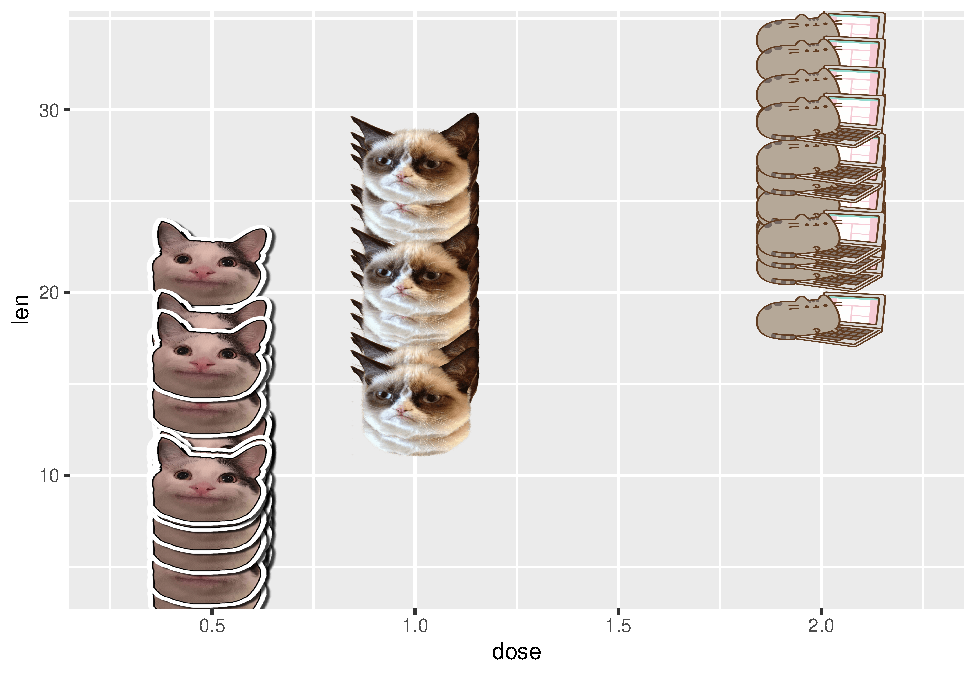
\includegraphics{_main_files/figure-latex/unnamed-chunk-230-1.pdf}

\subsection{\texorpdfstring{Misceláneos: \emph{ggtexttable()}}{Misceláneos: ggtexttable()}}\label{misceluxe1neos-ggtexttable}

Esta función me permite hacer mis tablas como figuras que puedo exportar como imágenes y darle formato.
Hace parte del paquete \textbf{ggpubr()} que vimos anteriormente.

Haremos un ejemplo con los primeros cuatro datos de \textbf{iris}:

\begin{Shaded}
\begin{Highlighting}[]
\FunctionTok{library}\NormalTok{(dplyr)}
\NormalTok{df}\OtherTok{\textless{}{-}}\NormalTok{ iris }\SpecialCharTok{\%\textgreater{}\%} \FunctionTok{slice}\NormalTok{(}\FunctionTok{c}\NormalTok{(}\DecValTok{1}\SpecialCharTok{:}\DecValTok{4}\NormalTok{))}
\FunctionTok{ggtexttable}\NormalTok{(df, }\AttributeTok{rows =} \ConstantTok{NULL}\NormalTok{)}
\end{Highlighting}
\end{Shaded}

\includegraphics{_main_files/figure-latex/unnamed-chunk-231-1.pdf}

También podemos cambiar el tema con el que se formatea la tabla, por ejemplo:

\begin{Shaded}
\begin{Highlighting}[]
\FunctionTok{ggtexttable}\NormalTok{(df, }\AttributeTok{rows =} \ConstantTok{NULL}\NormalTok{, }\AttributeTok{theme =} \FunctionTok{ttheme}\NormalTok{(}\StringTok{"blank"}\NormalTok{))}
\end{Highlighting}
\end{Shaded}

\includegraphics{_main_files/figure-latex/unnamed-chunk-232-1.pdf}

\begin{Shaded}
\begin{Highlighting}[]
\FunctionTok{ggtexttable}\NormalTok{(df, }\AttributeTok{rows =} \ConstantTok{NULL}\NormalTok{, }\AttributeTok{theme =} \FunctionTok{ttheme}\NormalTok{(}\StringTok{"light"}\NormalTok{))}
\end{Highlighting}
\end{Shaded}

\includegraphics{_main_files/figure-latex/unnamed-chunk-232-2.pdf}

\begin{Shaded}
\begin{Highlighting}[]
\FunctionTok{ggtexttable}\NormalTok{(df, }\AttributeTok{rows =} \ConstantTok{NULL}\NormalTok{, }\AttributeTok{theme =} \FunctionTok{ttheme}\NormalTok{(}\StringTok{"classic"}\NormalTok{))}
\end{Highlighting}
\end{Shaded}

\includegraphics{_main_files/figure-latex/unnamed-chunk-232-3.pdf}

\begin{Shaded}
\begin{Highlighting}[]
\FunctionTok{ggtexttable}\NormalTok{(df, }\AttributeTok{rows =} \ConstantTok{NULL}\NormalTok{, }\AttributeTok{theme =} \FunctionTok{ttheme}\NormalTok{(}\StringTok{"minimal"}\NormalTok{))}
\end{Highlighting}
\end{Shaded}

\includegraphics{_main_files/figure-latex/unnamed-chunk-232-4.pdf}

\begin{Shaded}
\begin{Highlighting}[]
\FunctionTok{ggtexttable}\NormalTok{(df, }\AttributeTok{rows =} \ConstantTok{NULL}\NormalTok{, }\AttributeTok{theme =} \FunctionTok{ttheme}\NormalTok{(}\StringTok{"lVioletWhite"}\NormalTok{))}
\end{Highlighting}
\end{Shaded}

\includegraphics{_main_files/figure-latex/unnamed-chunk-232-5.pdf}

\begin{Shaded}
\begin{Highlighting}[]
\FunctionTok{ggtexttable}\NormalTok{(df, }\AttributeTok{rows =} \ConstantTok{NULL}\NormalTok{, }\AttributeTok{theme =} \FunctionTok{ttheme}\NormalTok{(}\StringTok{"mVioletWhite"}\NormalTok{))}
\end{Highlighting}
\end{Shaded}

\includegraphics{_main_files/figure-latex/unnamed-chunk-232-6.pdf}

Para ver otros temas: \url{https://rpkgs.datanovia.com/ggpubr/files/ggtexttable-theme.pdf}

Otros formateos:

\begin{itemize}
\item
  Poner en negrita una celda:

\begin{Shaded}
\begin{Highlighting}[]
\FunctionTok{ggtexttable}\NormalTok{(df, }\AttributeTok{rows =} \ConstantTok{NULL}\NormalTok{,  }\AttributeTok{theme =} \FunctionTok{ttheme}\NormalTok{(}\StringTok{"classic"}\NormalTok{)) }\SpecialCharTok{\%\textgreater{}\%}  
  \FunctionTok{table\_cell\_font}\NormalTok{(}\AttributeTok{row =} \DecValTok{3}\NormalTok{, }\AttributeTok{column =} \DecValTok{2}\NormalTok{, }\AttributeTok{face =} \StringTok{"bold"}\NormalTok{, }\AttributeTok{color =} \StringTok{"red"}\NormalTok{)}
\end{Highlighting}
\end{Shaded}

  \includegraphics{_main_files/figure-latex/unnamed-chunk-234-1.pdf}
\item
  Resaltar una columna:

\begin{Shaded}
\begin{Highlighting}[]
\FunctionTok{ggtexttable}\NormalTok{(df, }\AttributeTok{rows =} \ConstantTok{NULL}\NormalTok{,  }\AttributeTok{theme =} \FunctionTok{ttheme}\NormalTok{(}\StringTok{"classic"}\NormalTok{)) }\SpecialCharTok{\%\textgreater{}\%} 
  \FunctionTok{table\_cell\_bg}\NormalTok{(}\AttributeTok{row =} \DecValTok{2}\SpecialCharTok{:}\DecValTok{5}\NormalTok{, }\AttributeTok{column =} \DecValTok{3}\NormalTok{, }\AttributeTok{fill=}\StringTok{"yellow"}\NormalTok{)}
\end{Highlighting}
\end{Shaded}

  \includegraphics{_main_files/figure-latex/unnamed-chunk-235-1.pdf}
\item
  Poner títulos y pies de notas:

\begin{Shaded}
\begin{Highlighting}[]
\FunctionTok{ggtexttable}\NormalTok{(df, }\AttributeTok{rows =} \ConstantTok{NULL}\NormalTok{,  }\AttributeTok{theme =} \FunctionTok{ttheme}\NormalTok{(}\StringTok{"classic"}\NormalTok{)) }\SpecialCharTok{\%\textgreater{}\%} 
  \FunctionTok{tab\_add\_title}\NormalTok{(}\AttributeTok{text =} \StringTok{"Data iris"}\NormalTok{,  }\AttributeTok{size =} \DecValTok{14}\NormalTok{, }\AttributeTok{face=}\StringTok{"bold"}\NormalTok{) }\SpecialCharTok{\%\textgreater{}\%}
  \FunctionTok{tab\_add\_footnote}\NormalTok{(}\AttributeTok{text =} \StringTok{"*Alguna nota"}\NormalTok{, }\AttributeTok{size =} \DecValTok{10}\NormalTok{, }\AttributeTok{face =} \StringTok{"italic"}\NormalTok{)}
\end{Highlighting}
\end{Shaded}

  \includegraphics{_main_files/figure-latex/unnamed-chunk-236-1.pdf}
\end{itemize}

\chapter{Valor de significancia p en estadística (p-value)}\label{valor-de-significancia-p-en-estaduxedstica-p-value}

\section{¿Qué es el valor p?}\label{quuxe9-es-el-valor-p}

\section{Interpretación general del valor p}\label{interpretaciuxf3n-general-del-valor-p}

\section{Marco de prueba de hipótesis: relación con la hipótesis nula y alternativa}\label{marco-de-prueba-de-hipuxf3tesis-relaciuxf3n-con-la-hipuxf3tesis-nula-y-alternativa}

\section{Regla de decisión: umbrales comunes para el valor p}\label{regla-de-decisiuxf3n-umbrales-comunes-para-el-valor-p}

\section{Errores en la prueba de hipótesis: error tipo I (falso positivo) y error tipo II (falso}\label{errores-en-la-prueba-de-hipuxf3tesis-error-tipo-i-falso-positivo-y-error-tipo-ii-falso}

\chapter{Introducción a la estadística}\label{introducciuxf3n-a-la-estaduxedstica}

\section{Diferencia entre estadística y bioestadística}\label{diferencia-entre-estaduxedstica-y-bioestaduxedstica}

\section{Estadística descriptiva: medidas de tendencia central y medidas de dispersión}\label{estaduxedstica-descriptiva-medidas-de-tendencia-central-y-medidas-de-dispersiuxf3n}

\section{Estadística inferencial: Univariada y multivariada}\label{estaduxedstica-inferencial-univariada-y-multivariada}

\section{Estadística inferencial paramétrica: supuestos principales de las pruebas paramétricas}\label{estaduxedstica-inferencial-paramuxe9trica-supuestos-principales-de-las-pruebas-paramuxe9tricas}

\section{Estadística inferencial no paramétrica: supuestos principales de las pruebas no paramétricas}\label{estaduxedstica-inferencial-no-paramuxe9trica-supuestos-principales-de-las-pruebas-no-paramuxe9tricas}

\section{¿Cómo saber si mis datos presentan una distribución normal y homogeneidad de las variancias?:}\label{cuxf3mo-saber-si-mis-datos-presentan-una-distribuciuxf3n-normal-y-homogeneidad-de-las-variancias}

\subsection{Prueba de Shapiro-Wilk}\label{prueba-de-shapiro-wilk}

\subsection{Pruebas de ajuste o distribución: Prueba de Kolmogorov-Smirnov, Prueba de Anderson-Darling}\label{pruebas-de-ajuste-o-distribuciuxf3n-prueba-de-kolmogorov-smirnov-prueba-de-anderson-darling}

\subsection{Prueba de Leven (varianzas).}\label{prueba-de-leven-varianzas.}

\emph{Data}

Para la revisión de los estadísticos básicos en R trabajaremos con el dataset \texttt{iris}.

\begin{Shaded}
\begin{Highlighting}[]
\FunctionTok{data}\NormalTok{(iris)}
\NormalTok{cols}\OtherTok{\textless{}{-}} \FunctionTok{c}\NormalTok{(}\StringTok{"Largo\_Sepalo"}\NormalTok{, }\StringTok{"Ancho\_Sepalo"}\NormalTok{, }\StringTok{"Largo\_Petalo"}\NormalTok{, }\StringTok{"Ancho\_Petalo"}\NormalTok{, }\StringTok{"Especies"}\NormalTok{)}
\FunctionTok{colnames}\NormalTok{(iris)}\OtherTok{\textless{}{-}}\NormalTok{ cols}
\end{Highlighting}
\end{Shaded}

Este conjunto de datos describe tres especies de las flores iris y como cambia el ancho y largo de su pétalo y sépalo.
Veamos la estructura de los datos:

\begin{Shaded}
\begin{Highlighting}[]
\FunctionTok{str}\NormalTok{(iris)}
\end{Highlighting}
\end{Shaded}

\begin{verbatim}
## 'data.frame':    150 obs. of  5 variables:
##  $ Largo_Sepalo: num  5.1 4.9 4.7 4.6 5 5.4 4.6 5 4.4 4.9 ...
##  $ Ancho_Sepalo: num  3.5 3 3.2 3.1 3.6 3.9 3.4 3.4 2.9 3.1 ...
##  $ Largo_Petalo: num  1.4 1.4 1.3 1.5 1.4 1.7 1.4 1.5 1.4 1.5 ...
##  $ Ancho_Petalo: num  0.2 0.2 0.2 0.2 0.2 0.4 0.3 0.2 0.2 0.1 ...
##  $ Especies    : Factor w/ 3 levels "setosa","versicolor",..: 1 1 1 1 1 1 1 1 1 1 ...
\end{verbatim}

\begin{Shaded}
\begin{Highlighting}[]
\FunctionTok{dim}\NormalTok{(iris)}
\end{Highlighting}
\end{Shaded}

\begin{verbatim}
## [1] 150   5
\end{verbatim}

\begin{Shaded}
\begin{Highlighting}[]
\FunctionTok{nrow}\NormalTok{(iris)}
\end{Highlighting}
\end{Shaded}

\begin{verbatim}
## [1] 150
\end{verbatim}

\begin{Shaded}
\begin{Highlighting}[]
\FunctionTok{ncol}\NormalTok{(iris)}
\end{Highlighting}
\end{Shaded}

\begin{verbatim}
## [1] 5
\end{verbatim}

Como vemos, posee 4 variables de respuesta y un factor que sería la especie de flor.

\includegraphics[width=0.5\linewidth]{images//flores}
\includegraphics[width=0.5\linewidth]{images//flores2}

\section{Estadísticos descriptivos}\label{estaduxedsticos-descriptivos}

Utilizando la función \texttt{summary()} podemos obtener información sobre nuestra data, como el valor mínimo, máximo, el promedio, la mediana y el rango intercuantil.

\begin{Shaded}
\begin{Highlighting}[]
\FunctionTok{summary}\NormalTok{(iris)}
\end{Highlighting}
\end{Shaded}

\begin{verbatim}
##   Largo_Sepalo    Ancho_Sepalo    Largo_Petalo    Ancho_Petalo         Especies 
##  Min.   :4.300   Min.   :2.000   Min.   :1.000   Min.   :0.100   setosa    :50  
##  1st Qu.:5.100   1st Qu.:2.800   1st Qu.:1.600   1st Qu.:0.300   versicolor:50  
##  Median :5.800   Median :3.000   Median :4.350   Median :1.300   virginica :50  
##  Mean   :5.843   Mean   :3.057   Mean   :3.758   Mean   :1.199                  
##  3rd Qu.:6.400   3rd Qu.:3.300   3rd Qu.:5.100   3rd Qu.:1.800                  
##  Max.   :7.900   Max.   :4.400   Max.   :6.900   Max.   :2.500
\end{verbatim}

\hfill\break
Si queremos estos datos por aparte o solo nos interesa estos y otros datos de la variable ``Largo\_Sepalo'', entonces usamos las funciones establecidas en R:\\

\begin{Shaded}
\begin{Highlighting}[]
\FunctionTok{mean}\NormalTok{(iris}\SpecialCharTok{$}\NormalTok{Largo\_Sepalo)}
\end{Highlighting}
\end{Shaded}

\begin{verbatim}
## [1] 5.843333
\end{verbatim}

\begin{Shaded}
\begin{Highlighting}[]
\FunctionTok{min}\NormalTok{(iris}\SpecialCharTok{$}\NormalTok{Largo\_Sepalo)}
\end{Highlighting}
\end{Shaded}

\begin{verbatim}
## [1] 4.3
\end{verbatim}

\begin{Shaded}
\begin{Highlighting}[]
\FunctionTok{max}\NormalTok{(iris}\SpecialCharTok{$}\NormalTok{Largo\_Sepalo)}
\end{Highlighting}
\end{Shaded}

\begin{verbatim}
## [1] 7.9
\end{verbatim}

\begin{Shaded}
\begin{Highlighting}[]
\FunctionTok{median}\NormalTok{(iris}\SpecialCharTok{$}\NormalTok{Largo\_Sepalo)}
\end{Highlighting}
\end{Shaded}

\begin{verbatim}
## [1] 5.8
\end{verbatim}

\begin{Shaded}
\begin{Highlighting}[]
\FunctionTok{quantile}\NormalTok{(iris}\SpecialCharTok{$}\NormalTok{Largo\_Sepalo, }\FloatTok{0.25}\NormalTok{) }\CommentTok{\# primer cuantil}
\end{Highlighting}
\end{Shaded}

\begin{verbatim}
## 25% 
## 5.1
\end{verbatim}

\begin{Shaded}
\begin{Highlighting}[]
\FunctionTok{quantile}\NormalTok{(iris}\SpecialCharTok{$}\NormalTok{Largo\_Sepalo, }\FloatTok{0.75}\NormalTok{) }\CommentTok{\# tercer cuantil}
\end{Highlighting}
\end{Shaded}

\begin{verbatim}
## 75% 
## 6.4
\end{verbatim}

\hfill\break
Otros estadísticos descriptivos\ldots{}\\

\begin{Shaded}
\begin{Highlighting}[]
\FunctionTok{sd}\NormalTok{(iris}\SpecialCharTok{$}\NormalTok{Largo\_Sepalo)  }\CommentTok{\#desviación estándar}
\end{Highlighting}
\end{Shaded}

\begin{verbatim}
## [1] 0.8280661
\end{verbatim}

\begin{Shaded}
\begin{Highlighting}[]
\FunctionTok{range}\NormalTok{(iris}\SpecialCharTok{$}\NormalTok{Largo\_Sepalo) }\CommentTok{\#min y max}
\end{Highlighting}
\end{Shaded}

\begin{verbatim}
## [1] 4.3 7.9
\end{verbatim}

\begin{Shaded}
\begin{Highlighting}[]
\FunctionTok{IQR}\NormalTok{(iris}\SpecialCharTok{$}\NormalTok{Largo\_Sepalo) }\CommentTok{\#diferencia entre el tercer y primer cuantil}
\end{Highlighting}
\end{Shaded}

\begin{verbatim}
## [1] 1.3
\end{verbatim}

\begin{Shaded}
\begin{Highlighting}[]
\FunctionTok{var}\NormalTok{(iris}\SpecialCharTok{$}\NormalTok{Largo\_Sepalo) }\CommentTok{\#varianza}
\end{Highlighting}
\end{Shaded}

\begin{verbatim}
## [1] 0.6856935
\end{verbatim}

\begin{Shaded}
\begin{Highlighting}[]
\FunctionTok{sd}\NormalTok{(iris}\SpecialCharTok{$}\NormalTok{Largo\_Sepalo) }\SpecialCharTok{/} \FunctionTok{mean}\NormalTok{(iris}\SpecialCharTok{$}\NormalTok{Largo\_Sepalo) }\CommentTok{\#Coeficiente variación}
\end{Highlighting}
\end{Shaded}

\begin{verbatim}
## [1] 0.1417113
\end{verbatim}

\hfill\break
Para conocer la desviación estándar de todas las columnas numéricas, usamos la función apply como anteriormente vimos:\\

\begin{Shaded}
\begin{Highlighting}[]
\FunctionTok{lapply}\NormalTok{(iris[, }\DecValTok{1}\SpecialCharTok{:}\DecValTok{4}\NormalTok{], sd)}
\end{Highlighting}
\end{Shaded}

\begin{verbatim}
## $Largo_Sepalo
## [1] 0.8280661
## 
## $Ancho_Sepalo
## [1] 0.4358663
## 
## $Largo_Petalo
## [1] 1.765298
## 
## $Ancho_Petalo
## [1] 0.7622377
\end{verbatim}

\newpage

\section{Gráficos descriptivos}\label{gruxe1ficos-descriptivos}

Si queremos explorar cómo es la variación de la longitud del sepalo por cada especie:\\

\begin{Shaded}
\begin{Highlighting}[]
\FunctionTok{boxplot}\NormalTok{(iris}\SpecialCharTok{$}\NormalTok{Largo\_Sepalo }\SpecialCharTok{\textasciitilde{}}\NormalTok{ iris}\SpecialCharTok{$}\NormalTok{Especies)}
\end{Highlighting}
\end{Shaded}

\begin{center}\includegraphics{_main_files/figure-latex/unnamed-chunk-245-1} \end{center}

\begin{Shaded}
\begin{Highlighting}[]
\FunctionTok{library}\NormalTok{(ggpubr)}
\FunctionTok{ggbarplot}\NormalTok{(}\AttributeTok{data =}\NormalTok{ iris, }\AttributeTok{x =} \StringTok{"Especies"}\NormalTok{, }\AttributeTok{y =} \StringTok{"Largo\_Sepalo"}\NormalTok{, }\AttributeTok{add =} \StringTok{"mean\_sd"}\NormalTok{)}
\end{Highlighting}
\end{Shaded}

\begin{center}\includegraphics{_main_files/figure-latex/unnamed-chunk-246-1} \end{center}

\hfill\break

\section{Explorando normalidad en los datos}\label{explorando-normalidad-en-los-datos}

Existen diversas gráficas que podemos realizar para probar o explorar si nuestros datos siguen una distribución normal (también llamada distribución gaussiana) y su gráfica debe tener una forma acampanada y simétrica.
La aplicación de muchas pruebas y estadísticos depende de si los datos siguen esta distribución o no.
Por esto es importante antes de aplicar cualquier prueba estadística, explorar la distribución de nuestros datos y sí la prueba o estadístico que aplicamos asume que nuestros datos sean normales o no.
Para este ejemplo, usaremos el ancho del sepalo en vez del largo del sepalo.
¨

\hfill\break

\begin{Shaded}
\begin{Highlighting}[]
\FunctionTok{hist}\NormalTok{(iris}\SpecialCharTok{$}\NormalTok{Ancho\_Sepalo)}
\end{Highlighting}
\end{Shaded}

\includegraphics{_main_files/figure-latex/unnamed-chunk-247-1.pdf}

\begin{Shaded}
\begin{Highlighting}[]
\FunctionTok{plot}\NormalTok{(}\FunctionTok{density}\NormalTok{(iris}\SpecialCharTok{$}\NormalTok{Ancho\_Sepalo))}
\end{Highlighting}
\end{Shaded}

\includegraphics{_main_files/figure-latex/unnamed-chunk-247-2.pdf}

\begin{Shaded}
\begin{Highlighting}[]
\FunctionTok{qqnorm}\NormalTok{(iris}\SpecialCharTok{$}\NormalTok{Ancho\_Sepalo)}
\FunctionTok{qqline}\NormalTok{(iris}\SpecialCharTok{$}\NormalTok{Ancho\_Sepalo)}
\end{Highlighting}
\end{Shaded}

\includegraphics{_main_files/figure-latex/unnamed-chunk-248-1.pdf}

\begin{Shaded}
\begin{Highlighting}[]
\FunctionTok{library}\NormalTok{(car) }\CommentTok{\# cargamos el paquete car}
\FunctionTok{qqPlot}\NormalTok{(iris}\SpecialCharTok{$}\NormalTok{Ancho\_Sepalo )}
\end{Highlighting}
\end{Shaded}

\includegraphics{_main_files/figure-latex/unnamed-chunk-249-1.pdf}

\begin{verbatim}
## [1] 16 34
\end{verbatim}

Al parecer nuestros datos tienen una distribución normal, según los gráficos, sin embargo, para estar seguros de esto, haremos una prueba llamada test de shapiro que nos permitirá confirmar esto:\\

\begin{Shaded}
\begin{Highlighting}[]
\FunctionTok{shapiro.test}\NormalTok{(iris}\SpecialCharTok{$}\NormalTok{Ancho\_Sepalo)}
\end{Highlighting}
\end{Shaded}

\begin{verbatim}
## 
##  Shapiro-Wilk normality test
## 
## data:  iris$Ancho_Sepalo
## W = 0.98492, p-value = 0.1012
\end{verbatim}

\hfill\break

La hipótesis nula que estamos aceptando o rechazando con esta prueba es que la distribución es normal y escogiendo un valor de probabilidad de 0.05 y dado que 0.1012 \textgreater{} 0.05 no podemos rechazar la hipótesis nula.
En caso que este valor de p-value \textless{} 0.05 entonces los datos no serían normales.

\section{Correlación y Regresión}\label{correlaciuxf3n-y-regresiuxf3n}

Correlación: Describe cómo dos variables están relacionadas.
Es una herramienta común para describir relaciones simples sin hacer afirmaciones sobre causa y efecto.
Estas relaciones pueden ser o no lineales, pero usualmente se busca o se desea saber si esta relación es lineal.

Por ejemplo queremos saber si existe una relación entre el largo y el ancho del pétalo de estas flores sin importar la especie:

\begin{Shaded}
\begin{Highlighting}[]
\FunctionTok{cor.test}\NormalTok{(iris}\SpecialCharTok{$}\NormalTok{Largo\_Petalo, iris}\SpecialCharTok{$}\NormalTok{Ancho\_Petalo)}
\end{Highlighting}
\end{Shaded}

\begin{verbatim}
## 
##  Pearson's product-moment correlation
## 
## data:  iris$Largo_Petalo and iris$Ancho_Petalo
## t = 43.387, df = 148, p-value < 2.2e-16
## alternative hypothesis: true correlation is not equal to 0
## 95 percent confidence interval:
##  0.9490525 0.9729853
## sample estimates:
##       cor 
## 0.9628654
\end{verbatim}

\hfill\break
Los valores que más nos interesan aquí son el \emph{cor} y el \emph{p-value}: Para un valor de cor de +1 quiere decir que dos variables están perfectamente correlacionadas positivamente.
Es decir, al aumentar una, aumenta la otra.
Un valor de -1 significa que las dos variables están perfectamente relacionadas negativamente, es decir, mientras una aumenta, la otra disminuye en la misma medida.
Un valor 0 significa que no hay correlación en las dos variables.
El valor p es la probabilidad de obentener un valor de cor más que extremo que el cor observado, dado los grados de libertad y si cor fuera 0.
Igualmente valores menores a 0.05 son significativos.
Hay otra función que nos permite obtener solo el coeficiente de correlación, de manera más práctica:\\

\begin{Shaded}
\begin{Highlighting}[]
\FunctionTok{cor}\NormalTok{(iris}\SpecialCharTok{$}\NormalTok{Largo\_Petalo, iris}\SpecialCharTok{$}\NormalTok{Ancho\_Petalo)                           }\CommentTok{\# si los datos son normales}
\end{Highlighting}
\end{Shaded}

\begin{verbatim}
## [1] 0.9628654
\end{verbatim}

\begin{Shaded}
\begin{Highlighting}[]
\FunctionTok{cor}\NormalTok{(iris}\SpecialCharTok{$}\NormalTok{Largo\_Petalo, iris}\SpecialCharTok{$}\NormalTok{Ancho\_Petalo, }\AttributeTok{method =} \StringTok{"spearman"}\NormalTok{)      }\CommentTok{\#si los datos no son normales}
\end{Highlighting}
\end{Shaded}

\begin{verbatim}
## [1] 0.9376668
\end{verbatim}

\hfill\break
Ahora bien, ya sabemos que estas dos variables están correlacionadas positivamente, así que si quiero construir un modelo que permite predecir valores en base a otros no medidos podemos aplicar una regresión lineal.
Una regresión lineal es un modelo lineal que describe la ecuación de dos variables de interés definidas en una función lineal: y = ax + b, donde a es la pendiente y b el intercepto.
La regresión lineal debe aplicarse sobre datos normales.
Así que chequemos la normalidad.
Primero, construimos el modelo y luego graficamos.
El modelo se construye con la variable de respuesta al lado izquiero de la ecuación y la variable que la explique a la derecha divididos por un signo de \textbf{``\textasciitilde{}''} .\\

\begin{Shaded}
\begin{Highlighting}[]
\NormalTok{modelo }\OtherTok{\textless{}{-}} \FunctionTok{lm}\NormalTok{(Ancho\_Petalo }\SpecialCharTok{\textasciitilde{}}\NormalTok{ Largo\_Petalo, }\AttributeTok{data =}\NormalTok{ iris) }
\FunctionTok{plot}\NormalTok{(modelo, }\AttributeTok{which =} \DecValTok{2}\NormalTok{)}
\end{Highlighting}
\end{Shaded}

\includegraphics{_main_files/figure-latex/unnamed-chunk-253-1.pdf}

Son solo pocos puntos que se salen de la gráfica, así que asumimos normalidad.

Exploremos el modelo:

\begin{Shaded}
\begin{Highlighting}[]
\FunctionTok{summary}\NormalTok{(modelo)}
\end{Highlighting}
\end{Shaded}

\begin{verbatim}
## 
## Call:
## lm(formula = Ancho_Petalo ~ Largo_Petalo, data = iris)
## 
## Residuals:
##      Min       1Q   Median       3Q      Max 
## -0.56515 -0.12358 -0.01898  0.13288  0.64272 
## 
## Coefficients:
##               Estimate Std. Error t value Pr(>|t|)    
## (Intercept)  -0.363076   0.039762  -9.131  4.7e-16 ***
## Largo_Petalo  0.415755   0.009582  43.387  < 2e-16 ***
## ---
## Signif. codes:  0 '***' 0.001 '**' 0.01 '*' 0.05 '.' 0.1 ' ' 1
## 
## Residual standard error: 0.2065 on 148 degrees of freedom
## Multiple R-squared:  0.9271, Adjusted R-squared:  0.9266 
## F-statistic:  1882 on 1 and 148 DF,  p-value: < 2.2e-16
\end{verbatim}

Con \emph{summary()} podemos ver los coeficientes de la ecuación, en este caso son: para el intercepto -0.36 y para la pendiente es 0.41.
De nuevo los valores p están por debajo de 0.05.
Los coeficientes son la pendiente y el intercepto.
Así que la ecuación queda -\textgreater{} Ancho\_Petalo = Largo\_Petalo*0.4157 - 0.3630

Otro resultado importante es el R cuadrado que nos dice la bondad del ajuste del modelo, esto es la fracción de mis datos que es explicado por el modelo en este caso si miramos el valor ajustado, el modelo explica el 92\% de mis datos.

\section{ANOVA (1 vía)}\label{anova-1-vuxeda}

ANOVA o análisis de varianza es un método estadístico que nos permite comparar las varianzas entre las medias (promedios) de diferentes grupos.

El ANOVA tiene varios supuestos: 1.
Independencia: cada observación es independiente de otra.
(Por ejemplo, si tenemos mediciones del mismo individuo a lo largo del tiempo, esta medida es dependiente al individuo).
2.
Normalidad : Que los datos siguen una distribución normal (como verificamos anteriormente).
3.
Homocedasticidad: varianzas equivalentes entre grupos.\\
Para la condición 1, en ningún lado nos dice que son muestras longitudinales, es decir, del mismo individuo a lo largo del tiempo, así que asumimos independencia.
Vamos a ver con estas dos gráficas si efectivamente se cumplen las condiciones 2 y 3.

\begin{Shaded}
\begin{Highlighting}[]
\NormalTok{modelo\_ancho }\OtherTok{\textless{}{-}} \FunctionTok{lm}\NormalTok{(Ancho\_Sepalo }\SpecialCharTok{\textasciitilde{}}\NormalTok{ Especies, }\AttributeTok{data =}\NormalTok{ iris) }
\FunctionTok{plot}\NormalTok{(modelo\_ancho, }\AttributeTok{which =} \FunctionTok{c}\NormalTok{(}\DecValTok{1}\NormalTok{,}\DecValTok{2}\NormalTok{) )}
\end{Highlighting}
\end{Shaded}

\includegraphics[width=0.45\linewidth]{_main_files/figure-latex/unnamed-chunk-255-1}
\includegraphics[width=0.45\linewidth]{_main_files/figure-latex/unnamed-chunk-255-2}

Este gráfico muestra si los residuos tienen patrones no lineales.
Si encuentra residuos igualmente distribuidos alrededor de una línea horizontal sin patrones distintos, es una buena indicación de que no tiene relaciones no lineales.
La linea roja debe ser más o menos recta, no debe estar curvada, entre más recta mejor.

\begin{Shaded}
\begin{Highlighting}[]
\FunctionTok{anova}\NormalTok{(modelo\_ancho)}
\end{Highlighting}
\end{Shaded}

\begin{verbatim}
## Analysis of Variance Table
## 
## Response: Ancho_Sepalo
##            Df Sum Sq Mean Sq F value    Pr(>F)    
## Especies    2 11.345  5.6725   49.16 < 2.2e-16 ***
## Residuals 147 16.962  0.1154                      
## ---
## Signif. codes:  0 '***' 0.001 '**' 0.01 '*' 0.05 '.' 0.1 ' ' 1
\end{verbatim}

En un sentido aplicado el número que más nos interesa es el valor F, sin embargo, se ha extendido la importancia del valor p que se define como la probabilidad de encontrar valores F más extremos que el observado y en este sentido la probabilidad es muy baja, mucho menor que el valor establecido como umbral que suele ser 0.05.
Así que rechazamos la hipótesis nula, lo que quiere decir que las medias de las especies son diferentes para el ancho del sépalo.

\section{Prueba de Tukey}\label{prueba-de-tukey}

ANOVA nos dice que hay diferencias en el ancho del sepalo por especie, pero no nos dice cual es más grande o cuales menor, o cual es diferente a cual.
Para esto hacemos una prueba de Tukey.
La función \texttt{aov()} realiza lo mismo que la de \texttt{anova()}.\\

\begin{Shaded}
\begin{Highlighting}[]
\NormalTok{fm1}\OtherTok{\textless{}{-}} \FunctionTok{aov}\NormalTok{(modelo\_ancho)}
\FunctionTok{TukeyHSD}\NormalTok{(fm1, }\StringTok{"Especies"}\NormalTok{, }\AttributeTok{ordered =} \ConstantTok{TRUE}\NormalTok{)}
\end{Highlighting}
\end{Shaded}

\begin{verbatim}
##   Tukey multiple comparisons of means
##     95% family-wise confidence level
##     factor levels have been ordered
## 
## Fit: aov(formula = modelo_ancho)
## 
## $Especies
##                       diff        lwr       upr     p adj
## virginica-versicolor 0.204 0.04314472 0.3648553 0.0087802
## setosa-versicolor    0.658 0.49714472 0.8188553 0.0000000
## setosa-virginica     0.454 0.29314472 0.6148553 0.0000000
\end{verbatim}

\hfill\break

\begin{Shaded}
\begin{Highlighting}[]
\FunctionTok{library}\NormalTok{(agricolae)}
\FunctionTok{HSD.test}\NormalTok{(fm1, }\StringTok{"Especies"}\NormalTok{, }\AttributeTok{group =} \ConstantTok{TRUE}\NormalTok{, }\AttributeTok{console =} \ConstantTok{TRUE}\NormalTok{)}
\end{Highlighting}
\end{Shaded}

\begin{verbatim}
## 
## Study: fm1 ~ "Especies"
## 
## HSD Test for Ancho_Sepalo 
## 
## Mean Square Error:  0.1153878 
## 
## Especies,  means
## 
##            Ancho_Sepalo       std  r        se Min Max   Q25 Q50   Q75
## setosa            3.428 0.3790644 50 0.0480391 2.3 4.4 3.200 3.4 3.675
## versicolor        2.770 0.3137983 50 0.0480391 2.0 3.4 2.525 2.8 3.000
## virginica         2.974 0.3224966 50 0.0480391 2.2 3.8 2.800 3.0 3.175
## 
## Alpha: 0.05 ; DF Error: 147 
## Critical Value of Studentized Range: 3.348424 
## 
## Minimun Significant Difference: 0.1608553 
## 
## Treatments with the same letter are not significantly different.
## 
##            Ancho_Sepalo groups
## setosa            3.428      a
## virginica         2.974      b
## versicolor        2.770      c
\end{verbatim}

\hfill\break
Esta función aparte de ver las diferencias de medias nos ordena con letras cual es la mayor y cual es la menor, veamoslo mejor en una gráfica de barras.\\

\includegraphics{_main_files/figure-latex/unnamed-chunk-259-1.pdf}

\newpage

\section{ANOVA (2 vías)}\label{anova-2-vuxedas}

El análisis de varianza de dos vías nos ayuda a estudiar la relación entre una variable dependiente cuantitativa y dos variables independientes cualitativas (factores) cada uno con varios niveles.
Este método hace todas las asunciones o supuestos que el ANOVA de 1 vía sobre normalidad y demás.
También es importante recalcar que para este tipo los grupos deben tener el mismo número de muestras o réplicas.
El ANOVA de dos vías permite estudiar cómo influyen por si solos cada uno de los factores sobre la variable dependiente (modelo aditivo) así como la influencia de las combinaciones que se pueden dar entre ellas (modelo con interacción).

\begin{itemize}
\item
  Modelo aditivo: aov(variable\_respuesta \textasciitilde{} factor1 + factor2, data)
\item
  Modelo con interacción: aov(variable\_respuesta \textasciitilde{} factor1 x factor2, data)\\
  Para este ejemplo usaremos el set de datos `ToothGrowth' con el que trabajamos la clase pasada.\\
\end{itemize}

\begin{Shaded}
\begin{Highlighting}[]
\FunctionTok{data}\NormalTok{(}\StringTok{"ToothGrowth"}\NormalTok{)}
\FunctionTok{str}\NormalTok{(ToothGrowth)}
\end{Highlighting}
\end{Shaded}

\begin{verbatim}
## 'data.frame':    60 obs. of  3 variables:
##  $ len : num  4.2 11.5 7.3 5.8 6.4 10 11.2 11.2 5.2 7 ...
##  $ supp: Factor w/ 2 levels "OJ","VC": 2 2 2 2 2 2 2 2 2 2 ...
##  $ dose: num  0.5 0.5 0.5 0.5 0.5 0.5 0.5 0.5 0.5 0.5 ...
\end{verbatim}

\hfill\break
Como podemos observar la variable de respuesta aquí sería la longitud de los dientes y los factores a evaluar son \emph{`supp'} y \emph{`dose'}, \emph{supp} es la forma en que le dieron la vitamia C a los cerdos, si como OJ (jugo de naranja) o AS (ácido ascórbico) a diferentes dosis (\emph{dose}) de 0.5, 1 y 2 mg/día.
El factor `dose' o dosis no aparece como factor sino como variable numérica.
Esto puede ser un inconveniente al correr el ANOVA así que modificaremos esto en la data.\\

\begin{Shaded}
\begin{Highlighting}[]
\NormalTok{ToothGrowth}\SpecialCharTok{$}\NormalTok{dose }\OtherTok{\textless{}{-}} \FunctionTok{factor}\NormalTok{(ToothGrowth}\SpecialCharTok{$}\NormalTok{dose, }
                  \AttributeTok{levels =} \FunctionTok{c}\NormalTok{(}\FloatTok{0.5}\NormalTok{, }\DecValTok{1}\NormalTok{, }\DecValTok{2}\NormalTok{),}
                  \AttributeTok{labels =} \FunctionTok{c}\NormalTok{(}\StringTok{"D0.5"}\NormalTok{, }\StringTok{"D1"}\NormalTok{, }\StringTok{"D2"}\NormalTok{))}
\FunctionTok{head}\NormalTok{(ToothGrowth)}
\end{Highlighting}
\end{Shaded}

\begin{verbatim}
##    len supp dose
## 1  4.2   VC D0.5
## 2 11.5   VC D0.5
## 3  7.3   VC D0.5
## 4  5.8   VC D0.5
## 5  6.4   VC D0.5
## 6 10.0   VC D0.5
\end{verbatim}

\hfill\break
Bien, visualizaremos nuestros datos para ver las tendencias de nuestros factores sobre nuestra variable de respuesta:\\
Boxplots
:

\begin{Shaded}
\begin{Highlighting}[]
\FunctionTok{library}\NormalTok{(ggpubr)}
\FunctionTok{ggboxplot}\NormalTok{(}\AttributeTok{data =}\NormalTok{ ToothGrowth, }\AttributeTok{x =} \StringTok{"supp"}\NormalTok{, }\AttributeTok{y =} \StringTok{"len"}\NormalTok{, }\AttributeTok{fill =} \StringTok{"supp"}\NormalTok{)}
\end{Highlighting}
\end{Shaded}

\includegraphics{_main_files/figure-latex/unnamed-chunk-262-1.pdf}

\begin{Shaded}
\begin{Highlighting}[]
\FunctionTok{ggboxplot}\NormalTok{(}\AttributeTok{data =}\NormalTok{ ToothGrowth, }\AttributeTok{x =} \StringTok{"dose"}\NormalTok{, }\AttributeTok{y =} \StringTok{"len"}\NormalTok{, }\AttributeTok{fill =} \StringTok{"dose"}\NormalTok{)}
\end{Highlighting}
\end{Shaded}

\includegraphics{_main_files/figure-latex/unnamed-chunk-262-2.pdf}

\begin{Shaded}
\begin{Highlighting}[]
\FunctionTok{ggboxplot}\NormalTok{(}\AttributeTok{data =}\NormalTok{ ToothGrowth, }\AttributeTok{x =} \StringTok{"dose"}\NormalTok{, }\AttributeTok{y =} \StringTok{"len"}\NormalTok{, }\AttributeTok{fill =} \StringTok{"supp"}\NormalTok{)}
\end{Highlighting}
\end{Shaded}

\includegraphics{_main_files/figure-latex/unnamed-chunk-262-3.pdf}

Líneas:

\begin{Shaded}
\begin{Highlighting}[]
\FunctionTok{ggline}\NormalTok{(ToothGrowth, }\AttributeTok{x =} \StringTok{"dose"}\NormalTok{, }\AttributeTok{y =} \StringTok{"len"}\NormalTok{, }\AttributeTok{color =} \StringTok{"supp"}\NormalTok{, }\AttributeTok{add =} \FunctionTok{c}\NormalTok{(}\StringTok{"mean\_se"}\NormalTok{, }\StringTok{"jitter"}\NormalTok{))}
\end{Highlighting}
\end{Shaded}

\includegraphics{_main_files/figure-latex/unnamed-chunk-263-1.pdf}

\hfill\break
Como pudimos ver aparentemente los factores podrían tener una interacción aunque muy level, en este caso podríamos correr una ANOVA dos vías o bien aditivo o bien mutiplicativo si queremos confirmar esta pequeña interacción.\\

\begin{Shaded}
\begin{Highlighting}[]
\NormalTok{anova1}\OtherTok{\textless{}{-}} \FunctionTok{aov}\NormalTok{(len }\SpecialCharTok{\textasciitilde{}}\NormalTok{ supp }\SpecialCharTok{+}\NormalTok{ dose, }\AttributeTok{data =}\NormalTok{ ToothGrowth)}
\NormalTok{anova2}\OtherTok{\textless{}{-}}  \FunctionTok{aov}\NormalTok{(len }\SpecialCharTok{\textasciitilde{}}\NormalTok{ supp }\SpecialCharTok{*}\NormalTok{ dose, }\AttributeTok{data =}\NormalTok{ ToothGrowth)}

\FunctionTok{summary}\NormalTok{(anova1)}
\end{Highlighting}
\end{Shaded}

\begin{verbatim}
##             Df Sum Sq Mean Sq F value   Pr(>F)    
## supp         1  205.4   205.4   14.02 0.000429 ***
## dose         2 2426.4  1213.2   82.81  < 2e-16 ***
## Residuals   56  820.4    14.7                     
## ---
## Signif. codes:  0 '***' 0.001 '**' 0.01 '*' 0.05 '.' 0.1 ' ' 1
\end{verbatim}

\begin{Shaded}
\begin{Highlighting}[]
\FunctionTok{summary}\NormalTok{(anova2)}
\end{Highlighting}
\end{Shaded}

\begin{verbatim}
##             Df Sum Sq Mean Sq F value   Pr(>F)    
## supp         1  205.4   205.4  15.572 0.000231 ***
## dose         2 2426.4  1213.2  92.000  < 2e-16 ***
## supp:dose    2  108.3    54.2   4.107 0.021860 *  
## Residuals   54  712.1    13.2                     
## ---
## Signif. codes:  0 '***' 0.001 '**' 0.01 '*' 0.05 '.' 0.1 ' ' 1
\end{verbatim}

\hfill\break
Como notamos tanto el modelo aditivo como multiplicativo, los factores explican de buena manera la varianza de nuestra variable.
Sin embargo en el modelo multiplicativo, que es el que nos muestra la interacción, nos dice que efectivamente hay una interacción entre nuestros factores (aunque muy pequeña), es decir, que el efecto de un factor depende del otro factor.

Las pruebas que realizamos anteriormente son de las comunes aplicadas para los conjuntos de datos, pero hay otras que podemos realizar también, por ejemplo en el caso de datos normales para hacer pruebas pareadas (dos niveles) podemos utilizar tambien \texttt{t.test}o en caso de no ser normales \texttt{wilcoxon.test}, en el caso de mas niveles para no parametricas podemos usar \texttt{kruskal.test}.
Por ejemplo:\\

\begin{Shaded}
\begin{Highlighting}[]
\CommentTok{\#dos niveles}
\FunctionTok{t.test}\NormalTok{(len }\SpecialCharTok{\textasciitilde{}}\NormalTok{ supp, }\AttributeTok{data =}\NormalTok{ ToothGrowth, }\AttributeTok{paired =} \ConstantTok{TRUE}\NormalTok{)}
\FunctionTok{wilcox.test}\NormalTok{(len }\SpecialCharTok{\textasciitilde{}}\NormalTok{ supp, }\AttributeTok{data =}\NormalTok{ ToothGrowth, }\AttributeTok{paired =} \ConstantTok{TRUE}\NormalTok{)}

\CommentTok{\#más de dos niveles}
\FunctionTok{kruskal.test}\NormalTok{(len }\SpecialCharTok{\textasciitilde{}}\NormalTok{ dose, }\AttributeTok{data =}\NormalTok{ ToothGrowth)}
\end{Highlighting}
\end{Shaded}

\hfill\break
Hay otras pruebas que se aplican dependiendo de los datos que tengamos y el objetivo de nuesto pregunta de investigación por ejemplo Dunn.test, Duncan.test, Welch.test, entre otros.
Hay muchos paquetes además de los que trae por default R stats (que viene por default con R) tales como \texttt{agricolae}, \texttt{vegan}, \texttt{emmeans} , entre otros, que vienen con más funciones y pruebas aplicadas a datos biológicos, ecológicos, entre otros.

\chapter{Tipos de pruebas paramétricas}\label{tipos-de-pruebas-paramuxe9tricas}

\section{Prueba t de una muestra}\label{prueba-t-de-una-muestra}

\section{Prueba t de dos muestras}\label{prueba-t-de-dos-muestras}

\section{Prueba t de Welch}\label{prueba-t-de-welch}

\section{Prueba F de Fisher}\label{prueba-f-de-fisher}

\section{Prueba t pareada}\label{prueba-t-pareada}

\section{ANOVA (one-way-anova, two-way-anova)}\label{anova-one-way-anova-two-way-anova}

\section{ANCOVA}\label{ancova}

\section{Correlación de Pearson}\label{correlaciuxf3n-de-pearson}

\section{Regresión lineal simple y múltiple}\label{regresiuxf3n-lineal-simple-y-muxfaltiple}

\section{Etc.}\label{etc.}

\chapter{Tipos de pruebas no paramétricas}\label{tipos-de-pruebas-no-paramuxe9tricas}

\section{Prueba de Mann-Whitney U (Wilcoxon rank-sum test)}\label{prueba-de-mann-whitney-u-wilcoxon-rank-sum-test}

\section{Prueba de Wilcoxon para muestras relacionadas}\label{prueba-de-wilcoxon-para-muestras-relacionadas}

\section{Prueba de Kruskal-Wallis}\label{prueba-de-kruskal-wallis}

\section{Prueba de Friedman}\label{prueba-de-friedman}

\section{Prueba de Chi-cuadrado (χ²)}\label{prueba-de-chi-cuadrado-ux3c7uxb2}

\section{Prueba de McNemar}\label{prueba-de-mcnemar}

\section{Correlación de rango de Spearman}\label{correlaciuxf3n-de-rango-de-spearman}

\section{Correlación de Kendall (τ de Kendall)}\label{correlaciuxf3n-de-kendall-ux3c4-de-kendall}

\chapter{Análisis de riqueza y diversidad alfa y beta}\label{anuxe1lisis-de-riqueza-y-diversidad-alfa-y-beta}

\chapter{Análisis multivariados}\label{anuxe1lisis-multivariados}

\section{PCA}\label{pca}

\section{PCoA}\label{pcoa}

\section{NMDS}\label{nmds}

\section{Permanova}\label{permanova}

\section{permdis}\label{permdis}

\section{Anosim}\label{anosim}

\section{RDA}\label{rda}

\section{CCA}\label{cca}

\chapter{Modelización estadística:}\label{modelizaciuxf3n-estaduxedstica}

\section{Modelo lineal general}\label{modelo-lineal-general}

\section{GLM con distribución Poisson}\label{glm-con-distribuciuxf3n-poisson}

\section{GLM con distribución quasi-Poisson}\label{glm-con-distribuciuxf3n-quasi-poisson}

\section{GLM con distribución de Bernoulli (Binomial)}\label{glm-con-distribuciuxf3n-de-bernoulli-binomial}

\section{GLMM: modelos lineales generales mixtos}\label{glmm-modelos-lineales-generales-mixtos}

\end{document}
